\documentclass[doctor%,final
]{iscs-thesis}

\usepackage[numbers,sort&compress]{natbib}
\def\NAT@spacechar{~}% NEW

%\usepackage{cleverref}
%\usepackage{hyperref}  % causes compile error
\usepackage{stmaryrd,setspace,float}
\usepackage[counterclockwise]{rotating}
\usepackage{enumitem}
\usepackage{textcomp}
\usepackage{makeidx}
\usepackage{caption}
\usepackage{subcaption}
\usepackage{begriff}
\usepackage{dsfont}
\usepackage{cmll}
\usepackage{tipa}

% \usepackage{tikz}
% \usepackage{tikz-cd}

\makeindex

%% from http://yav.purely-functional.net/haskell_latex.html
\usepackage{fancyvrb}
\DefineVerbatimEnvironment{code}{Verbatim}{fontsize=\small}
\DefineVerbatimEnvironment{spec}{Verbatim}{fontsize=\small}
\newcommand{\ignore}[1]{}


\usepackage{rotating}

\usepackage{bussproofs,stmaryrd}
\usepackage{showlabels}
\EnableBpAbbreviations

%%% from haskell symposium submitted paper
\usepackage{graphicx}
\usepackage{amssymb,amsmath}
\usepackage{amscd}

\usepackage[amsmath,standard,thref,thmmarks]{ntheorem}

% \doublespacing

\newcommand{\Nat}{{\mathbb N}}
\newcommand{\Real}{{\mathbb R}}
\newcommand{\pvar}{\mathsf{PVar}}
\newcommand{\agents}{\mathcal A}
\newcommand{\wvar}{\mathsf{WVar}}

\newcommand{\tuple}[1]{\langle{#1}\rangle}
\newcommand{\fix}[1]{[FIX \fbox{#1}]}
\newcommand{\fml}{\mathsf{\operatorname{Fml}}}
\newcommand{\id}{\operatorname{id}}
\newcommand{\kv}{$\mathbf K \vee$}
\newcommand{\vdashR}{\vdash_{\mathsf R}}

\newcommand{\vdashRLB}{\vdashR^{\mbox{\tiny \LB}}}

\newcommand{\T}{\mathbf T}
\newcommand{\memory}{{\sf m}}
\newcommand{\ruleskip}{\vskip 5mm}

%%%

\newcommand{\R}[1]{{#1}^{\mathsf R}}
\newcommand{\modelsR}{\models_{\mathsf R}}


\newtheorem{notation}{Notation}

\newcommand{\nat}{\mathbb{N}}
\newcommand{\steps}[2]{Steps_{#1}\left({#2}\right)}

\newcommand{\hypc}[2]{{\mathcal{C}#1}\left[{#2}\right]}
\newcommand{\hyper}{\mathcal{H}}
\newcommand{\hypert}{\mathcal{O}}
\newcommand{\hmid}{\ \ \rule[-2pt]{2pt}{9pt}\ \ }

\newcommand{\tr}{\vdash}
\newcommand{\update}{\vartriangleleft}

\newcommand{\elim}{\mathcal E}
\newcommand{\intro}{\mathcal I}

\newcommand{\coml}{\leftarrow_{\mathrm g}}
\newcommand{\comr}{\leftarrow_{\mathrm d}}

\newcommand{\reduce}{\rightsquigarrow}
\newcommand{\reduction}{\reduce^\ast}
\newcommand{\processes}{\mathbb{P}}
\newcommand{\ProV}{\mathsf{ProV}}
\newcommand{\LB}{\textbf{LB}}
\newcommand{\p}[1]{\texttt{#1}}

%% terms
\newcommand{\lpair} [1]{\langle{#1}\rangle}
\newcommand{\cotuple}[1]{[{#1}]}
\newcommand{\ev}[1]{\mathsf{ev}\left({#1}\right)}

\newcommand{\inl}[1]{\mathsf{inl}({#1})}
\newcommand{\inr}[1]{\mathsf{inr}({#1})}

\newcommand{\linl}[1]{\mathsf{inl}\left({#1}\right)}
\newcommand{\linr}[1]{\mathsf{inr}\left({#1}\right)}

\newcommand{\lpil}[1]{\pi_{\mathsf l}\left({#1}\right)}
\newcommand{\lpir}[1]{\pi_{\mathsf r}\left({#1}\right)}

\newcommand{\mats}[6]{\langle \inl{#1}. ({#2},{#3})/ \inr{#4}. ({#5},{#6})\rangle}
\newcommand{\mat} [5]{\mathsf{match}\,{#1}\,\mathsf{of}\, \inl{#2}. {#3}/
\inr{#4}. {#5}}

\newcommand{\ifte}[3]{\mathsf{If}\, {#1}\, \mathsf{then}\, {#2}\,
\mathsf{else}\, {#3}}

\newcommand{\abort}{\mathsf{abort\,}}

\newcommand{\compare}[2]{{#1} == {#2}}

\newcommand{\term} [0]{M}
\newcommand{\lterm}[0]{\mathcal{T}^-}
\newcommand{\val}  [0]{\mathcal{V}}
\newcommand{\lval} [0]{\mathcal{V}^-}
\newcommand{\tj}   [2]{ {#1} \mathord{\colon\kern -2pt}{#2} }

\newcommand{\wor}{\,\mathbin{\mathsf{or}}\,}

\newcommand{\Id}{\mathsf{Id}}
\newcommand{\lgd}{$\lambda$-GD}

%% configuration
\newcommand{\lstore}{{S}}
\newcommand{\conf}[2]{(\lstore{#1},{#2})}
\newcommand{\confwithcontext}[3]{\conf{#1}{#2}{\hypert\hmid C[{{#3}}]\hmid\hypert'}}
\newcommand{\concreteconf}[2]{({#1},{#2})}

%% reductions and the like
\newcommand{\breduce}{\reduce_{\mathrm B}}
\newcommand{\areduce}{\reduce_{\mathrm A}}
\newcommand{\wreduce}{\reduce_{\mathrm W}}
\newcommand{\rreduce}{\reduce_{\mathrm R}}
\newcommand{\preduce}{\reduce_{\mathrm P}}
\newcommand{\bpreduce}{\reduce_{\mathrm{B/P}}}

%% logical rules
\newcommand{\UnaryRule}[3]{ \AxiomC{#1}
\LeftLabel{#2}
\UnaryInfC{#3} \DisplayProof}
\newcommand{\BinaryRule}[4]{ \AxiomC{#1} \AxiomC{#2}
\LeftLabel{#3}
\BinaryInfC{#4}\DisplayProof}
\newcommand{\TrinaryRule}[5]{ \AxiomC{#1} \AxiomC{#2}
\AxiomC{#3} \LeftLabel{#4}
\TrinaryInfC{#5} \DisplayProof}

%% investi
\newcommand{\inv}[1]{{#1}^{\mathsf i}}

\newcommand{\rightlocal}{\rightsquigarrow_{\beta{\mathrm l}}}
\newcommand{\rightcomm}{\rightsquigarrow_{\beta{\mathrm c}}}
\newcommand{\rightdist}{\rightsquigarrow_{\beta{\mathrm d}}}
\newcommand{\dist}[2]{[{#1}; {#2}]}

\newcommand{\interpret}[1]{\llbracket {#1} \rrbracket}

\newcommand{\process}{p}
\newcommand{\contex}[1]{\mathcal C[{#1}]}
\newcommand{\semo}[1]{\llbracket{#1}\rrbracket}
\newcommand{\semoi}[1]{\llparenthesis{#1}\rrparenthesis}
\newcommand{\semi}[1]{\llparenthesis{#1}\rrparenthesis}

\newcommand{\wwedge}{\operatorname*{\bigwedge\kern -8pt \bigwedge}}

% macros
\newcommand {\G}{\Gamma}
\newcommand {\D}{\Delta}

\renewcommand{\phi}{\varphi}
\newcommand{\imp}{\supset}

\newcommand{\bbot}{
    \mathord{\reflectbox{\rotatebox[origin=c]{-90}{$\models$}}}}

\newcommand{\form}{\mathop{\text{Form}}}

\newcommand{\ruleT}[1]{\LeftLabel{(T)}\UnaryInfC{${#1}$}}
\newcommand{\powerset}[1]{{\mathcal P({#1})}}
\newcommand{\proj}[0]{\operatorname{proj}}
\newcommand{\len}[0]{\operatorname{len}}
\newcommand{\cl}[0]{\operatorname{cl}}
\newcommand{\carrier}[0]{\operatorname{carrier}}
\newcommand{\subfml}{\operatorname{subfml}}
\newcommand{\seq}{\operatorname{Seq}}
\newcommand{\type}{\operatorname{Type}}
\newcommand{\vdashsc}{\vdash_{\mbox{\rm sc}}}
\newcommand{\iec}{{\rm {\textbf{IEC}}}}
\newcommand{\ckv}{{\rm {\textbf{S4}\ast\cdots\ast\textbf{S4}}}}
\newcommand{\vdashsf}{\vdash_{\ckv}}
\newcommand{\initial}[1]{${#1}\vdashn{#1}$}
\newcommand{\supsete}[1]{\LeftLabel{($\supset$-E)}\BinaryInfC{${#1}$}}
\newcommand{\supseti}[1]{\LeftLabel{($\supset$-I)}\UnaryInfC{${#1}$}}
\newcommand{\nec}[1]{\LeftLabel{(nec)}\UnaryInfC{${#1}$}}
\newcommand{\wedgeel}[1]{\LeftLabel{($\wedge$-E$_0$)}\UnaryInfC{${#1}$}}
\newcommand{\wedgei}[1]{\LeftLabel{($\wedge$-I)}\BinaryInfC{${#1}$}}
\newcommand{\veeil}[1]{\LeftLabel{($\vee$-I$_0$)}\UnaryInfC{${#1}$}}
\newcommand{\veeir}[1]{\LeftLabel{($\vee$-I$_1$)}\UnaryInfC{${#1}$}}
\newcommand{\veee}[1]{\LeftLabel{($\vee$-E)}\TrinaryInfC{${#1}$}}
\newcommand{\weaken}[1]{\LeftLabel{(w)}\UnaryInfC{${#1}$}}
\newcommand{\be}[1]{\LeftLabel{($\bot$-E)}\UnaryInfC{${#1}$}}
\newcommand{\ax}[1]{	     \AxiomC{}
	     \LeftLabel{(ax)}
\UnaryInfC{\initial{#1}}}
\newcommand{\dn}[1]{\LeftLabel{(DN)}\UnaryInfC{${#1}$}}

\newcommand{\xphi}{\tj{x}{\phi}}
\newcommand{\ypsi}{\tj{y}{\psi}}

\newcommand{\rev}[1]{{#1}^{-1}}

\newcommand{\sem}[1]{|{#1}|}
\newcommand{\nsem}[1]{\sem{#1}^-}
\newcommand{\sempair}[1]{\sem{(#1)}}

\renewcommand{\vec}{\overrightarrow}
\newcommand{\sche}{\sqsubseteq}


\newcommand{\sequent}[2]{{#1}\tr{#2}}
\newcommand{\aseq}[2]{\AxiomC{$\sequent{#1}{#2}$}}
\newcommand{\useq}[2]{\UnaryInfC{$\sequent{#1}{#2}$}}
\newcommand{\bseq}[2]{\BinaryInfC{$\sequent{#1}{#2}$}}
\newcommand{\tseq}[2]{\TrinaryInfC{$\sequent{#1}{#2}$}}

\newcommand{\limp}{\multimap}

\newcommand{\conc}{\parallel}
\newcommand{\comod}[2]{\ast^{\rightarrow {#2}}_{\leftarrow{#1}}}
\newcommand{\reader}[1]{\ast_{\leftarrow{#1}}}

\newcommand{\sred}{\succ_{\mathsf s}}
\newcommand{\ared}{\succ_{\mathsf a}}
\newcommand{\red}{\succ}

\newcommand{\comodL}{\comod c{\co c}}
\newcommand{\comodR}{\comod{\co c}{c}}

\newcommand{\sLambda}{\Lambda_{\mathsf s}}
\newcommand{\aLambda}{\Lambda_{\mathsf a}}
\newcommand{\sPi}{\Pi_{\mathsf s}}
\newcommand{\aPi}{\Pi_{\mathsf a}}
\newcommand{\FLe}{FL$_{\mathrm {e}}$}
\newcommand{\MTLs}{MTL$_{\mathrm{s}}$}
\newcommand{\bu}[1]{{#1}^\bullet}
\newcommand{\HLBCK}{\mathbf{HL}^\forall_{\mathbf{BCK}}}

\newcommand{\NMTL}{\mathbf{N}_{\mathbf{MTL2}}}
\newcommand{\NMLL}{\mathbf{N}_{\mathbf{IMLL2}}}

\newcommand{\eH}{e_{\hatma H}}
\newcommand{\eI}{e_{\hatma I}}
\newcommand{\hatma}[1]{\hat{\mathcal{#1}}}
\newcommand{\takehyper}[1]{e_{#1}\in \semo{#1}}
\newcommand{\eHz}{e_{\mathrm{H0}}}
\newcommand{\eHo}{e_{\mathrm{H1}}}

\newcommand{\co}[1]{\bar{#1}}

\newcommand{\letpar}[4]{\mathsf{let}\, {#1} \,\mathsf{be}\, ({#2}\conc
{#3})\, \mathsf{in}\, {#4}}

\newcommand{\brac}[1]{\lbrack {#1}\rbrack}

\newcommand{\imapsto}[1]{\{i\mapsto {#1}\}}
\newcommand{\kmapsto}[1]{\{k\mapsto {#1}\}}
\newcommand{\mmapsto}[1]{\{m\mapsto {#1}\}}
\newcommand{\jmapsto}[1]{\{j\mapsto {#1}\}}

\newcommand{\bool}{\mathbb{B}}

\newcommand{\dom}{\mathop{\mathrm{dom}}}
\newcommand{\FV}{\mathrm{FV}}

\newcommand{\one}{\mathbf{1}}
\newcommand{\letin}[3]{\mathsf{let }\,{#1}\,\mathsf{ be
}\,{#2}\,\mathsf{ in }\,{#3}}
\newcommand{\ign}[2]{\mathsf{ign }\,{#1}\,\mathsf{ in }\,{#2}}

\newcommand{\eval}{\Downarrow}

\newcommand{\terminate}{\mathsf{end}}

\newcommand{\sendtype}[2]{\tuple{#1}.{#2}}
\newcommand{\recvtype}[2]{(#1).{#2}}

\newcommand{\sendterm}[3]{{#1}\langle{#2}\rangle.{#3}}
\newcommand{\recvterm}[3]{{{#1}({#2}).{#3}}}

\newcommand{\leftside }[1]{\mathop\triangleright(#1)}
\newcommand{\rightside}[1]{\mathop\triangleleft(#1) }
\newcommand{\bothside}[1]{\mathop{\triangleright\triangleleft}(#1) }

\newcommand{\hypere}{\mathcal{E}}

\newcommand{\two}{\one\oplus\one}
\etitle{Hyper-Lambda Calculi}
\jtitle{$B%O%$%Q!<%i%`%@7W;;(B}
\eauthor{Yoichi Hirai}
\jauthor{$BJ?0fMN0l(B}
\esupervisor{Masami Hagiya}
\jsupervisor{$BGkC+>;8J(B}
\supervisortitle{Professor} % Professor, etc.
\date{\fix{XXX}}

\begin{document}

\begin{eabstract}
 We propose hyper-lambda calculi.  A hyper-lambda term is a finite
 sequence of lambda terms, representing concurrent processes.  We give
 two concrete hyper-lambda calculi: synchronous and asynchronous.  Both
 employ a
 pair of communication primitives exchanging their inputs.
 In the synchronous case, both sides succeed.  In the asynchronous case,
 at least one side obtains the other side's input.
 The synchronous calculus denotes message-passing communication
 and session types;
 the asynchronous calculus characterizes shared-memory waitfree
 communication.
 Among processes of a typed hyper-lambda term,
 all succeed in the synchronous case while
 at least one succeeds in the asynchronous case.
 Logically, the processes are interpreted conjunctively
 in the synchronous case but disjunctively in the asynchronous case.
 The synchronous calculus is based on our original Amida logic:
 $(\phi\limp\psi)\otimes(\psi\limp\phi)$ on top of intuitionistic linear
 logic;
 the asynchronous calculus is based on G\"odel--Dummett logic:
 $(\phi\imp\psi)\lor(\psi\imp\phi)$ on top of intuitionistic logic.
 These calculi are in Curry--Howard correspondence with the
 hypersequent-style natural deduction.
\end{eabstract}

\begin{jabstract}
 $B%O%$%Q!<%7!<%1%s%H7W;;$K4p$/%O%$%Q!<%i%`%@7W;;$rDs0F$9$k!#(B
 $B%i%`%@7W;;$,%i%`%@9`$r<B9T$9$k!#(B
 $B%O%$%Q!<%i%`%@7W;;$O%i%`%@9`$NNs$r<B9T$9$k!#(B
 $B%i%`%@9`$NNs$OJBNs<B9T$5$l$k%9%l%C%I$rI=$9!#(B
 $B%O%$%Q!<%i%`%@7W;;$NM-MQ@-$r<($9$?$a$K(B
 $BFs$D$NNc$r<($9!#(B

 $B:G=i$NNc$O!"%A%c%M%k$r7PM3$7$?(B
 $BF14|DL?.$N$?$a$N%O%$%Q!<%i%`%@7W;;$G$"$k!#(B
 $B%O%$%Q!<%i%`%@9`$KB0$9$k(B
 $B$9$Y$F$N%9%l%C%I$N<B9T$,(B
 $B@.N)$9$k$3$H$r7?%7%9%F%`$,J]>Z$9$k!#(B
 $B7?%7%9%F%`$H$7$FL$CN$NO@M}$r:NMQ$9$k!#(B
 $BD>4Q<g5A@~7AO@M}$K8xM}(B$(\phi\limp\psi)\otimes(\psi\limp\phi)$$B$rDI2C$7$?(B
 $BO@M}$K$D$$$F(BCurry--Howard$BBP1~$r$H$C$F%O%$%Q!<%i%`%@7W;;$H$7$F$_$?$H$3$m!"(B
 $B%W%m%;%97W;;$N%W%m%;%9$d%;%C%7%g%s7?$r%^%/%m$H$7$F<BAu$G$-$?!#(B

 $B<!$NNc$O!"6&M-%a%b%j$r7PM3$7$?(B
 $BHsF14|DL?.$N$?$a$N%O%$%Q!<%i%`%@7W;;$G$"$k!#(B
 $B%O%$%Q!<%i%`%@9`$KB0$9$k(B
 $B>/$/$H$b0l$D$N%9%l%C%I$N<B9T$,(B
 $B@.N)$9$k$3$H$r7?%7%9%F%`$,J]>Z$9$k!#(B
 $B7?%7%9%F%`$O!"(B1950$BG/Be$+$iCN$i$l$F$$$k(B
 $B%2!<%G%k!&%@%a%C%HO@M}$G$"$k!#(B
 $B%2!<%G%k!&%@%a%C%HO@M}$K$D$$$F(BCurry--Howard$BBP1~$r$H$C$F(B
 $B%O%$%Q!]%i%`%@7W;;$H$7$F$_$?$H$3$m!"(B
 $BJ,;67W;;$NLdBj%/%i%9$G$"$k(Bwaitfree$B7W;;$rFCD'$E$1$i$l$?!#(B
 $B%2!<%G%k!&%@%a%C%HO@M}$b(Bwaitfree$B7W;;$b!$$=$l$>$l$NJ,Ln$G=EMW$G$"$k$N$K!$(B
 $B$3$l$i$N4XO"$O!$$3$l$^$GCN$i$l$F$$$J$+$C$?!%(B

 $B%2!<%G%k!&%@%a%C%HO@M}$OCf(B
 $B4VO@M}(B($BD>4Q<g5AO@M}$H8EE5O@M}$N4V$NO@M}(B)$B$N0l$D$G$"$k!%(BWaitfree$B7W;;$O!$%W%m%;%9$,B>$N(B
 $B%W%m%;%9$rBT$F$J$$$H$$$&@)8B$G7h$^$k!$J,;67W;;$N%/%i%9$G$"$k!%(B
 $BK\8&5f$N9W8%$O!$%2!<%G%k!&%@%a%C%HO@M}$N7?IU$-%i%`%@7W;;$rDj5A$7$F!$(B
 $B$A$g$&$I(Bwaitfree$B7W;;$G2r$1$kLdBj$@$1$r2r$1$k$H<($7$?$3$H$G$"$k!%(B
 $BK\8&5f$O!$(B
 $B6&M-%a%b%j$N0l4S@-$r!$7?%7%9%F%`$GFCD'$E$1$?=i$a$F$N8&5f$G$"$C$F!$(B
 $B6=$j$D$D$"$k!VHsL@<(%a%b%j0l4S@-!W$H8F$V$Y$-8&5fJ,Ln$N=EMW$J0lJb$G$"$k!%(B

 $BCx<T$O=$;NO@J8$G!$%2!<%G%k!&%@%a%C%HO@M}$H6&M-%a%b%j0l4S@-$N0l<o$G$"$k(B
 $BC`<!0l4S@-$H$N0UL#O@E*$J4XO"$K5$$E$$$F$$$?!%(B
 $B$7$+$7!$K\8&5f$N<jK!$bLdBj$b(B
 Arnon Avron$B$N(B1991$BG/$NO@J8$K$h$k$H$3$m$,Bg$-$$!%(B
 $B$^$:!$$=$NO@J8$G(BAvron$B$,Ds0F$7$?%O%$%Q!<%7!<%1%s%H$,!$(B
 $BK\8&5f$N7?IU$-%i%`%@7W;;$N4pAC$G$"$k!%(B
 $B$5$i$K!$$=$NO@J8$G(BAvron$B$,Ds5/$7$?LdBj(B
 $B!V%O%$%Q!<%7!<%1%s%H$G%+%C%H=|5n$G$-$kO@M}$N7W;;E*0UL#$O$J$K$+!W(B
 $B$,!$K\8&5f$GC55a$9$kLdBj$G$"$k!%(B
 $B$3$NFs==G/Mh$NLdBj$NE57?Nc$G$"$k%2!<%G%k!&%@%a%C%HO@M}$N>l9g$K!$2rEz$r(B
 $BM?$($k!%%2!<%G%k!&%@%a%C%HO@M}$N7W;;E*0UL#$O!$(Bwaitfree$B7W;;$G$"$k$H<($9!%(B

 $B5;=QE*$K!$K\8&5f$O7?IU$-%i%`%@7W;;$N8&5f$G$"$k!%(B
 $B<($7$?DjM}$O!$(B
 $B7?$,IU$$$?9`$N4JLs$,L58B$KB3$+$J$$$3$H$H!$(B
 $B7?$,IU$$$?9`$N4JLs$,<:GT$rI=$99`$G=*$o$i$J$$$3$H$H!$(B
 $B7?$,IU$$$?9`$G2r$1$kLdBj$,(Bwaitfree$B$K2r$1$kLdBj$H(B
 $B0lCW$9$k$3$H$N;0$D$G$"$k!%(B

 \fix{$B:G=*E*$K1Q8l$K9g$o$;$l$P$$$$(B}
\end{jabstract}


\maketitle

\begin{acknowledge}
 This research was partially supported by
 Grant-in-Aid for JSPS Fellows, 23-6978, 2011.

 The work about Hyper $\lambda$ calculus is encouraged by feedbacks from
 ACAN (Algebraic and
 Coalgebraic
 Approaches to
 Non-Classical Logics Workshop) and OPLSS'11 participants,
 \fix{Pisa}
 \fix{FLOPS}
 and numerous less formal occasions.

 My second and third years of PhD course were
 supported by Grant-in-Aid for JSPS Fellows 23-6978.
 This thesis partly prepared during the author's stay in
 ILPS, the University of Amsterdam, during which the author was supported
 by the same JSPS grant.

 Tadeusz Litak informed the author of Danos and Krivine's paper
 ``Disjunctive Tautologies as Synchronisation Schemes''

 The author thank Tadeusz Litak for informing the author of
 Danos and Krivine's work.

 Emacs and YaTeX mode.
\end{acknowledge}


\frontmatter
\tableofcontents

\listoffigures

\chapter*{List of Examples}
\theoremlisttype{allname}
\listtheorems{example}

\chapter*{List of Theorems}
\theoremlisttype{allname}
\listtheorems{theorem,corollary}

\vskip 3mm
\noindent
For definitions, see Index at the end of the thesis.

% \listoftables

\mainmatter

\chapter{Introduction}

\subsection{Our Contributions}

We propose hyper-lambda calculi.
Instead of lambda terms in ordinary lambda calculi,
we use a finite sequence of lambda terms called hyper-lambda terms.
We give two such examples:
one models synchronous send--receive communication (Chapter~\ref{ch:exchange}) and
the other models asynchronous waitfree
read--write communication (Chapter~\ref{ch:lambda}).
We also give an example of hyper-lambda calculi style programming in Haskell.
The two hyper-lambda calculi are in Curry--Howard correspondence with
hypersequent formulation of logics: Amida logic and G\"odel--Dummett
logic.
G\"odel--Dummett logic is an intermediate logic.
An intermediate logic is a logic \textit{between} classical and
intuitionistic logics, where `between' is defined using the
set-theoretic inclusion of valid logical formulae of each logic.
Amida logic is a substructural logic.

\citet{hosoi-ono} declared that they chose to study intermediate
logics in
general rather than studying specific intermediate logics.
However, concrete results about specific subjects matter when the
results contain new phenomena.
This thesis is intended to contain such concrete discoveries
about specific intermediate and substructural logics.

The famous logic among th two,
G\"odel--Dummett logic, is
a typical intermediate logic logic known from 1950's.
Our method is the Curry--Howard correspondence, also known from 1940's.
Our result is characterization of waitfreedom, a concept in the theory
of distributed computation extensively studied in 1990's.
Since both sides of the correspondence is already known,
the discovery is a replay of Curry's surprise.

Of course, there have been many instances of Curry--Howard correspondence.

We list our contributions from the most important:
\begin{enumerate}
 \item developing a lambda calculus using
       a hypersequent calculus (Chapters~\ref{ch:lambda,ch:exchange});
 \item identifying the computational ability of the
       G\"odel--Dummett logic with waitfreedom (Chapter~\ref{ch:lambda});
 \item encoding session types using a seemingly unknown axiom
       $(p\limp q)\otimes(q\limp p)$ (which we call Amida axiom) on top
       of intuitionistic linear logic (Chapter~\ref{ch:exchange}),
 \item discovery of Amida logic (Chapter~\ref{ch:exchange});
 \item using conjunctive hypersequents for the first time (Chapter~\ref{ch:exchange}).
\end{enumerate}

Our first contribution is the technique for our first contribution.
We developed a lambda calculus based on \citet{avron91}'s hypersequents.
\citet{avron91} himself noted that it would be important to develop a
lambda calculus for hypersequents.
The lambda calculus relies on \citet{avron91}'s hypersequents.
The hypersequent calculus is a
variant of the deduction system called sequent calculus.  In sequent
calculus, each step of a proof tree concludes a sequent $\G\vdash\phi$ that
consists of a finite sequence of logical formulae~$\G$ and a logical
formula~$\phi$.  The sequent $\G\vdash\phi$ is
interpreted as an implication.  In hypersequent calculus, each step of a
proof tree concludes a hypersequent instead of a sequent.  A
hypersequent is a sequence of sequents delimited by $\hmid$:
$\G\vdash\phi\hmid \D\vdash\psi
\hmid \cdots$.  Also here, each component is interpreted as an
implication, and then the whole hypersequent is interpreted as the
disjunction of all those implications.
When we interpret proofs as programs, we take the components as
concurrent processeses.  Following the original disjunctive
interpretation of components, we regard the proof tree as the guarantee of
success of at least one process.

Our second contribution is finding a way to interpret proofs in
G\"odel--Dummett logic as
concurrently executable programs for waitfree computation.
Although \citet{avron91} noticed his hypersequent calculus has something
to do with concurrency (as the title of~\citep{avron91} contains the phrase
``intermediate logics for concurrency''), it was unknown that
the computational interpretation of G\"odel--Dummett logic has
the degree of synchronization called waitfreedom.  This discovery
constitutes our first contribution.

According to \citet[p.97]{curryhoward},
the Curry--Howard isomorphism~\citep{curryhoward} was first made
precise by \citet[\textbf{9}E and
\textbf{9}F]{curry1974combinatory}.
The intuitionistic propositional logic and the typed lambda calculus
had been independently invented but Curry discovered them to be the same thing.
The ``double discovery'' (\citet{wadler2012propositions}) is considered
to affirm the importance of the typed lambda calculi.
In this thesis we witness a replay of the ``double discovery'' with
different casts: G\"odel--Dummett logic and the waitfreedom.
Both of these were born in the early eras of their respective academic
disciplines:
mathematical logic bore G\"odel Dummett logic in
1950's~\citep{dummett59}
and the computer science bore waitfree computation in
1970's~\citep{lamport1979make}.
Chapter~\ref{ch:exchange} is about the unknown connection between these two.

This is the first such computational
interpretation for intermediate logics (Fig.~\ref{fig:lattice}).
Another significance of this contribution
is giving interpretation of nondterminism in typed
lambda calculi.  In the simply typed lambda calculus for intuitionistic
propositional logic, all typed terms have a unique normal form.
However, in typed lambda calculi for classical propositional logic,
there can be multiple normal forms unless we employ an evaluation
strategy or limit the set of reductions.
The lack of unique normal forms in the classical propositional proofs
has puzzled logicians for decades. \fix{mention Lafont's example; say it
is a matter of concurrency}
 \begin{figure}
  \centering
  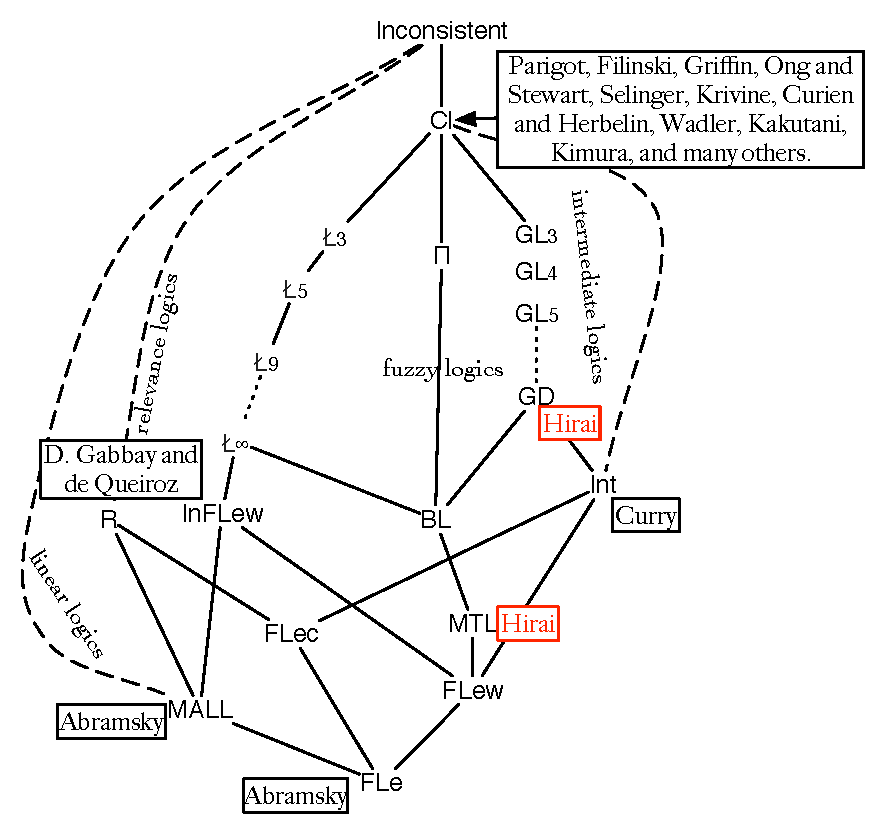
\includegraphics[scale=0.8]{lattice.eps}
  \caption[The lattice of substructural logics, some of which with known lambda calculi.]
  {The substructural logics for which lambda calculi are found.
  The underlying Hasse diagram of well-known substructural logics is
  taken from
  \cite[p.~120]{residuated} with slight modifications.
  The names in boxes refer to people who developed lambda calculi for
  these logics.
  \textsf{GD} stands for G\"odel--Dummett logic, for which
  a lambda calculus will be given in
  Chapter~\ref{ch:lambda}.
  \textsf{Amida} stands for the Amida logic, an original logic
  defined in Chapter~\ref{ch:exchange}.
  \textsf{MTL} stands for monoidal t-norm logic~\citep{Esteva2001271},
  for which a lambda calculus will be given
  in Chapter~\ref{ch:pole}.
  \textsf{FLe} is for the full Lambek calculus with exchange
  rule~\citep[p.86]{residuated}, which is also known as the
  intuitionistic
  multiplicative additive fragment of linear logic (IMALL).
  \textsf{MALL} stands for its classical version, the multiplicative
  additive fragment of linear logic.  For these fragments of linear
  logic,
  \citet{abramsky1993computational} gave lambda calculi.
  \textsf{FLew} stands for the full Lambek calculus with exchange and
  weakening,
  which is also known as intuitionistic affine logic.
  Affine logics lack contraction, which causes exponential size increase
  during cut-elimination process.
  Asperti gave light affine logic~\citep{2002}.
  \citet{terui2007} gave an affine typed lambda calculus for polynomial
  time computation.
  \textsf{R} stands for relevance logic~\citep{urquhart1972},
  for which \citet{gabbay1992} gave a lambda calculus.
  \textsf{Int} stands for the intuitionistic propositional logic.
  The original Curry--Howard isomorphism was found for this logic by
  Curry~\citep{curry1942}.
  \textsf{Cl} stands for the classical propositional logic.
  There is intensive research going on for the computational
  interpretation of classical logic.  Namely,
  Parigot's $\lambda\mu$-calculus~\citep{lambdamu},
  Filinski's symmetric lambda calculus~\citep{filinski1989},
  Griffin's control perator~$\mathcal C$~\citep{griffin1990},
  Ong and Stewart's $\lambda\mu_{\mathrm
  v}$~\citep{ong-stewart},
%   \citet{bb1994}, this is predicate logic
  Selinger's categorical semantics and duality
  result~\citep{selinger2001} for which \citet{kakutani2002} introduced
  fixed-point
  operators,
  Curien and Herbelin's $\bar\lambda\mu\tilde\mu$
  calculus~\citep{curien2000},
  Wadler's dual calculus~\citep{wadler-dual, wadler-reloaded} and so on.
  For the history of lambda calculi for classical logic,
  Daisuke Kimura's thesis~\cite{kimura} is a source of detailed
  information.
  \textsf{Inconsistent} stands for the logic of all logical formulae.
  A programming language \texttt{Haskell}, which is based on
  the typed lambda calculi, has
  an inconsistent type system.
  }
  \label{fig:lattice}
 \end{figure}

Our third contribution is

Our fourth contribution is

Our fifth contribution is

\fix{turn this into a table, linear or intuitionistic, conjunction or disjunction}
The previous works treated the computational interpretations of
disjunctive formulae like $(\phi\imp\psi)\lor(\psi\imp\phi)$ or
$(\phi\limp\psi)\oplus(\psi\limp\phi)$.  In this chapter, we try
replacing these disjunctions with conjunctions.
In the former case, the change renders the logic inconsistent.
If we add the axiom $(\phi\imp\psi)\land(\psi\imp\phi)$ to the
intuitionistic propositional logic,
we can prove any formula.  However in the lattar case, the change does
not make the system meaningless.
In this chapter, we treat
the axioms of the form $(\phi\limp\psi)\otimes(\psi\limp\phi)$
on top of IMLL2, the second order formulation of intuitionistic
multiplicative linear
logic.  In essence, the axiom allows two processes to wait for one
another and then exchange information.

The content of Chapter~\ref{ch:lambda} appears in
a conference paper by the author \citep{hiraiflops2012}
although we have applied substantial modifications since then.

% \section{An Introduction for Computer Scientists}

% \section{An Introduction for Proof Theorists}

% \section{An Introduction for Functional Programmers}

% \section{An Introduction for Philosophers}


  \subsection{Preliminaries and Notations}

  We assume inductive definitions using BNF and coinductive definition.
  $\powerset X$ denotes the powerset of $X$.
  For a symbol or a sequence of symbols $p$,
  $p^+$ denotes repetition of $p$ more than zero times and
  $p^*$ denotes repetition of $p$ more than or equal to zero times.

\chapter{The Logic of Information Exchange}
\label{ch:exchange}

\subsection{Summary}

After studying $(\phi\limp\psi)\oplus (\psi\limp\phi)$,
it is natural to change the additive disjunction $\oplus$ into
multiplicative conjunction $\otimes$ and see what happens%
\footnote{Takeuti Izumi asked what about conjunctions.}.
A natural way to add $(\phi\limp\psi)\otimes(\psi\limp\phi)$ as an axiom
is adding a pair of primitives $\lpair{c,\co c}$ so that
$\cdots ct \cdots \co c u \cdots$ reduces to
$\cdots u  \cdots t \cdots$: in words,
$c$ outputs $\co c$'s input and vice versa.
However, there is one problem: what happens to $\co c(c t)$?
In this case, we do not know the output of $c$ because we only have an
equality between $\co c$'s input and $c$'s output.
Fortunately, we just want to know the output of $\co c$, which is the
input of $c$, that is, $t$.

axiom

usual exchange

nested

nested more complicated

The previous chapters treated the computational interpretations of
disjunctive formulae like $(\phi\imp\psi)\lor(\psi\imp\phi)$ or
$(\phi\limp\psi)\oplus(\psi\limp\phi)$.  In this chapter, we try
replacing these disjunctions with conjunctions.
In the former case, the change renders the logic inconsistent.
If we add the axiom $(\phi\imp\psi)\land(\psi\imp\phi)$ to the
intuitionistic propositional logic,
we can prove any formula.  However in the lattar case, the change does
not make the system meaningless.
In this chapter, we treat
the axioms of the form $(\phi\limp\psi)\otimes(\psi\limp\phi)$
on top of IMLL2, the second order formulation of intuitionistic
multiplicative linear
logic.  In essence, the axiom allows two processes to wait for one
another and then exchange information.

\section{Definitions}

\subsection{Terms and Free Variables}

\fix{channels, involution}

Following Abramsky \fix{cite}, we defne patterns binding sets of
variables:
\begin{itemize}
 \item $\ast$ and $\_$ are patterns binding $\emptyset$,
 \item $\lpair{x,\_}$, $\lpair{\_,x}$ and $!x$ are patterns binding
       $\{x\}$,
 \item $x\otimes y$ and $x@y$ are patterns binding $\{x,y\}$.
\end{itemize}
Using patterns, we define a term $t$ with free variables~$S$ inductively:
\begin{itemize}
 \item a variable $x$ is a term with free variables $\{x\}$,
 \item $\ast$ is a term with free variables $\emptyset$,
 \item if $t$ is a term with free variables~$X$, $u$ is a term with
       free variables~$Y$ and $X$ and $Y$ are disjoint, $t\otimes u$ and
       $tu$ are terms with free variables $X\cup Y$,
 \item if $t$ and $u$ are terms with free variables $X$, then
       $\lpair{t,u}$ is a term with free variables~$X$,
 \item if $t$ is a term with free variables~$X$, then
       $\inl x, \inr t$ and $!t$ are terms with free variables~$X$
 \item if $t$ is a term with free variables $X\cup \{x\}$ and $x$ is not
       in $X$, then $\lambda x.t$ is a term with free variables~$X$,
 \item if $t$ is a term with free variables~$X$, $p$ is a pattern
       binding $Y$, $u$ is a term with free variables $Y\cup Z$ and
       $X\cap Z = Y\cap Z = \emptyset$, then,
       $\letin t p u$ is a term with free variables $X\cup Z$,
 \item if $t$ is a term with free variables $X$,
       $u$ is a term with free variables $Z\cup \{x\}$,
       $v$ is a term with free variables $Z\cup \{y\}$,
       $x,y\notin Z$ and $X\cap Z = \emptyset$,
       $\mat t x u y v$ is a term with free variables $X\cup Z$, and
 \item channels are terms with free variables~$\emptyset$.
\end{itemize}
Note that a term with free variables $X$ is not a term with free
variables $Y$ when $X\neq Y$.  Only the last clause is original,
introducing channels, which are our communication primitives.

\subsection{Typing Derivations}

On top of Abramsky's \fix{} we add a rule to make
$(\phi\limp\psi)\otimes(\psi\limp\phi)$ derivable\fix{really?}.

The typing rules are in Figure~\ref{fig:exchange:rules}.
 \begin{figure}
  \centering
  % axiom
  \AxiomC{}
  \LL{Ax}
  \UnaryInfC{$\tj{x}{\phi}\tr\tj{x}{\phi}$}
  \DisplayProof
  %
  \hfill \fix{add external exchange} \hfill
  % exchange
  \AxiomC{$\hypert\hmid\G,\tj{x}{\phi},\tj{y}{\psi},\D\tr\tj{t}{\theta}$}
  \LL{IE}
  \UnaryInfC{$\hypert\hmid\G,\tj{y}{\psi},\tj{x}{\phi},\D\tr\tj{t}{\theta}$}
  \DisplayProof
  %
  \ruleskip
  \AxiomC{$\hypert$}
  \AxiomC{$\hypert'$}
  \LL{merge}
  \BinaryInfC{$\hypert\hmid\hypert'$}
  \DisplayProof
  % cut XXX is this necessary?; yes
  \hfill
  \AxiomC{$\hypert\hmid\G\tr\tj{t}{\phi}\hmid\tj{x}{\phi},\D\tr\tj{u}{\psi}$}
  \LL{Cut}
  \UnaryInfC{$\hypert\hmid\G,\D\tr\tj{u[t/x]}{\psi}$}
  \DisplayProof
  %
  \ruleskip
  % 1R
  \AxiomC{}
  \LL{$\one$R}
  \UnaryInfC{$\tr\tj{\ast}{\one}$}
  \DisplayProof
  %
  \hfill
  % 1L
  \AxiomC{$\hypert\hmid\G\tr\tj{t}{\phi}$}
  \LL{$\one$L}
  \UnaryInfC{$\hypert\hmid\G,\tj{z}{\one}\tr\tj{\letin z \ast t}{\phi}$}
  \DisplayProof
  %
  \ruleskip
  % otimes R
  \AxiomC{$\hypert\hmid\G\tr\tj{t}{\phi}\hmid\D\tr\tj{u}{\psi}$}
  \LL{$\otimes$R}
  \UnaryInfC{$\hypert\hmid\G,\D\tr\tj{t\otimes u}{\phi\otimes \psi}$}
  \DisplayProof
  %
  \hfill
  % sync
  \AxiomC{$\hypert\hmid\G\tr\tj{t}{\phi}\hmid \D\tr\tj{u}{\psi}$}
  \LL{sync}
  \UnaryInfC{$\hypert\hmid
  \G\tr\tj{ct}{\psi}\hmid \D\tr\tj{\co cu}{\phi}$}
  \DisplayProof
  %
  \ruleskip
  % otimes L
  \AxiomC{$\hypert\hmid\G,\tj{x}{\phi},\tj{y}{\psi}\tr\tj{t}{\theta}$}
  \LL{$\otimes$L}
  \UnaryInfC{$\hypert\hmid\G,\tj{z}{\phi\otimes\psi}\tr\tj{\letin{z}{x\otimes
  y}{t}}{\theta}$}
  \DisplayProof
  %
  \ruleskip
  % limp R
  \AxiomC{$\hypert\hmid\G,\tj{x}{\phi}\tr\tj{t}{\psi}$}
  \LL{$\limp$R}
  \UnaryInfC{$\hypert\hmid\G\tr\tj{\lambda x.t}{\phi\limp \psi}$}
  \DisplayProof
  %
  \hfill
  % limp L
  \AxiomC{$\hypert\hmid\G\tr\tj{t}{\phi}\hmid\tj{x}{\psi},\D\tr\tj{u}{\theta}$}
  \LL{$\limp$L}
  \UnaryInfC{$\hypert\hmid\G,\tj{f}{\phi\limp\psi},\D\tr \tj{u[(ft)/x]}{\theta}$}
  \DisplayProof
  %
  \ruleskip
  % andR
  \AxiomC{$\hypert\hmid\G\tr\tj{t}{\phi}\hmid\G\tr\tj{u}{\psi}$}
  \LL{$\with$R}
  \UnaryInfC{$\hypert\hmid\G\tr\tj{\lpair{t,u}}{\phi\with\psi}$}
  \DisplayProof
  %
  \ruleskip
  % andL0
  \AxiomC{$\hypert\hmid\G,\tj{x}{\phi}\tr\tj{t}{\theta}$}
  \LL{$\with$L$_0$}
  \UnaryInfC{$\hypert\hmid\G,\tj{z}{\phi\with\psi}\tr\tj{\letin{z}{\lpair{x,\_}}{t}}{\theta}$}
  \DisplayProof
  %
  \ruleskip
  % andL1
  \AxiomC{$\hypert\hmid\G,\tj{y}{\psi}\tr\tj{t}{\theta}$}
  \LL{$\with$L$_1$}
  \UnaryInfC{$\hypert\hmid\G,\tj{z}{\phi\with\psi}\tr\tj{\letin{z}{\lpair{\_,y}}{t}}{\theta}$}
  \DisplayProof
  %
  \ruleskip
  % oplus R0
  \AxiomC{$\hypert\hmid\G\tr\tj{t}{\phi}$}
  \LL{$\oplus$R$_0$}
  \UnaryInfC{$\hypert\hmid\G\tr\tj{\inl{t}}{\phi\oplus\psi}$}
  \DisplayProof
  %
  \hfill
  % oplus R1
  \AxiomC{$\hypert\hmid\G\tr\tj{u}{\psi}$}
  \LL{$\oplus$R$_1$}
  \UnaryInfC{$\hypert\hmid\G\tr\tj{\inr{u}}{\phi\oplus\psi}$}
  \DisplayProof
  %
  \ruleskip
  % oplus L
  \AxiomC{$\hypert \hmid \G,\tj{x}{\phi}\tr\tj{u}{\theta}\hmid
  \G,\tj{y}{\psi}\tr\tj{v}{\theta}$}
  \LL{$\oplus$L}
  \UnaryInfC{$\hypert\hmid\G,\tj{z}{\phi\oplus\psi}\tr\tj{\mat{z}{x}{u}{y}{v}}{\theta}$}
  \DisplayProof
  %
  \ruleskip
  % !R
  \AxiomC{$\hypert\hmid!\G\tr\tj{t}{\phi}$}
  \LL{$!$R}
  \UnaryInfC{$\hypert\hmid!\G\tr\tj{!t}{!\phi}$}
  \DisplayProof
  %
  \ruleskip
  % dereliction
  \AxiomC{$\hypert\hmid\G,\tj{x}{\phi}\tr\tj{t}{\psi}$}
  \LL{Dereliction}
  \UnaryInfC{$\hypert\hmid\G,\tj{z}{!\phi}\tr\tj{\letin{z}{!x}{t}}{\psi}$}
  \DisplayProof
  %
  \ruleskip
  % contraction
  \AxiomC{$\hypert\hmid\G,\tj{x}{!\phi},\tj{y}{!\phi}\tr\tj{t}{\psi}$}
  \LL{Contraction}
  \UnaryInfC{$\hypert\hmid\G,\tj{z}{!\phi}\tr\tj{\letin{z}{x@y}{t}}{\psi}$}
  \DisplayProof
  %
  \ruleskip
  % weakening
  \AxiomC{$\hypert\hmid\G\tr\tj{t}{\psi}$}
  \LL{Weakening}
  \UnaryInfC{$\hypert\hmid\G,\tj{z}{!\phi}\tr\tj{\letin{z}{\_}{t}}{\psi}$}
  \DisplayProof
  %
  \ruleskip
  % forall R
  \AxiomC{$\hypert\hmid\G\tr\tj{t}{\phi}$}
  \LL{$\forall$R}
  \UnaryInfC{$\hypert\hmid\G\tr\tj{t}{\forall X.\phi}$}
  \DisplayProof (No $X$ appears in $\G$)
  %
  \ruleskip
  % forall L
  \AxiomC{$\hypert\hmid\G,\tj{x}{\phi[\psi/X]}\tr\tj{t}{\phi}$}
  \LL{$\forall$L}
  \UnaryInfC{$\hypert\hmid\G,\tj{x}{\forall X.\phi}\tr\tj{t}{\phi}$}
  \DisplayProof
  %
  \ruleskip
  %
  \caption{Most rules are taken from Abramsky\fix{}.
  The sync rule is original.}
  \label{fig:exchange:rules}
 \end{figure}

\subsection{Evaluation relation}

The set of canonical forms remains the same as Abramsky's
system~\fix{cite}:
\[
 \lpair{t,u}\qquad !t\qquad \ast\qquad c\otimes d\qquad \lambda
 x.t\qquad \inl{v}\qquad\inr{w}
\]
where $v$ and $w$ are canonical forms.

$\mathcal E$ stands for a sequence of evaluation relations.
Most rules are the same as Abramsky's \fix{cite}.
We add the semantics for channels.
The definition is inductive in Figure~\ref{fig:eval}.

\newcommand{\hypere}{\mathcal{E}}

 \begin{figure}
  \centering
  \AxiomC{}
  \UnaryInfC{$\ast\eval\ast$}
  \DisplayProof
  \hfill
  \AxiomC{$\hypere\hmid t\eval \ast \hmid u\eval v$}
  \UnaryInfC{$\hypere\hmid \letin t \ast u\eval v$}
  \DisplayProof
  \hfill
  \AxiomC{$\hypere\hmid t\eval v\hmid u\eval w$}
  \UnaryInfC{$\hypere\hmid t\otimes u\eval v\otimes w$}
  \DisplayProof
  \ruleskip
  \AxiomC{$\hypere\hmid t\eval v\otimes d\hmid u[v/x,w/y]\eval v'$}
  \UnaryInfC{$\hypere\hmid \letin t {x\otimes y} u \eval v'$}
  \DisplayProof
  \hfill
  \AxiomC{}
  \UnaryInfC{$\lambda x.t\eval \lambda x.t$}
  \DisplayProof
  \ruleskip
  \AxiomC{$\hypere\hmid t\eval \lambda x.t'\hmid u\eval v\hmid
  t'[v/x]\eval w$}
  \UnaryInfC{$\hypere\hmid tu\eval w$}
  \DisplayProof
  \hfill
  \AxiomC{$\hypere\hmid t\eval v\hmid u\eval w$}
  \UnaryInfC{$\hypere\hmid ct\eval w\hmid \co cu\eval v$}
  \DisplayProof
  \ruleskip
  \AxiomC{}
  \UnaryInfC{$\lpair{t,u}\eval\lpair{t,u}$}
  \DisplayProof
  \hfill
  \AxiomC{$\hypere\hmid t\eval \lpair{t_0,t_1}\hmid t_0\eval v\hmid
  u[v/x]\eval w$}
  \UnaryInfC{$\letin t {\lpair{x,\_}}{u}\eval w$}
  \DisplayProof
  \ruleskip
  \AxiomC{$\hypere\hmid t\eval\lpair{t_0,t_1}\eval t_1\eval v\hmid
  u[v/y]\eval w$}
  \UnaryInfC{$\hypere\hmid\letin t{\lpair{\_,y}}u\eval w$}
  \DisplayProof
  \ruleskip
  \AxiomC{$\hypere\hmid t\eval v$}
  \UnaryInfC{$\hypere\hmid \inl{t}\eval \inl{v}$}
  \DisplayProof
  \hfill
  \AxiomC{$\hypere\hmid u\eval w$}
  \UnaryInfC{$\hypere \hmid \inr{u}\eval \inr{w}$}
  \DisplayProof
  \ruleskip
  \AxiomC{$\hypere\hmid t\eval \inl{v}\hmid u[v/x]\eval w$}
  \UnaryInfC{$\hypere\hmid \mat t x u y {u'}\eval w$}
  \DisplayProof
  \ruleskip
  \AxiomC{$\hypere\hmid t\eval \inr{v}\hmid u'[v/y]\eval w$}
  \UnaryInfC{$\hypere\hmid \mat t x u y {u'}\eval w$}
  \DisplayProof
  \ruleskip
  \AxiomC{}
  \UnaryInfC{$\hypere\hmid !t\eval !t$}
  \DisplayProof
  \hfill
  \AxiomC{$\hypere\hmid t\eval !s\hmid s\eval v\hmid u[v/x]\eval w$}
  \UnaryInfC{$\hypere \hmid \letin t {!x} u\eval w$}
  \DisplayProof
  \ruleskip
  \AxiomC{$\hypere\hmid t\eval !s\hmid u\eval v$}
  \UnaryInfC{$\hypere \hmid \letin t {\_} u\eval v$}
  \DisplayProof
  \hfill
  \AxiomC{$\hypere\hmid t\eval !s\hmid u[!s/x,!s/y]\eval v$}
  \UnaryInfC{$\letin t {x@y} u\eval v$}
  \DisplayProof
  \caption{The definition of evaluation relation.}
  \label{fig:eval}
 \end{figure}

\section{Determinacy and Confluence}


\section{Conclusion}


\section{Discussion}

It is tempting to add modalities to types so that the
modalities show agents and then study the relationship with the
multiparty session types \fix{cite}.
\renewcommand{\comodL}{\comod cd}
\renewcommand{\comodR}{\comod dc}

\chapter{A Hyper $\lambda$-Calculus for G\"odel--Dummett Logic}
\label{ch:lambda}

\subsection{Summary}

We propose a typed lambda calculus based on Avron's hypersequent
calculus~\citep{avron91} for G\"odel--Dummett logic.  This calculus
turns out to model
waitfree computation~\citep{Herlihy88,Saks:1993vq}.
Besides strong normalization and non-abortfullness,
we give soundness and completeness of
the calculus against the typed version of waitfree protocols.
The calculus is not only proof theoretically interesting,
but also valuable as a basis for distributed programming languages.

The Curry--Howard isomorphism~\cite{curryhoward} is surprising because the same
method works for two different purposes: a logical purpose of
removing redundancy from proofs and a computational purpose of finding a
class of terminating programs.
We extend
this surprise to G\"odel--Dummett logic and
waitfreedom.
G\"odel--Dummett logic~\cite{dummett59}
is one of the intermediate logics
between classical and intuitionistic logics.
Waitfreedom~\cite{Herlihy88,Saks:1993vq} is a class of distributed
computation without synchronization among processes.

We connect G\"odel--Dummett logic and waitfreedom using
Avron's hypersequent calculus~\cite{avron91}.
In doing that, we respond to his suggestion:
\begin{quote}
it seems to us extremely important to determine the exact
       computational content of them~[intermediate logics] ---
       and {to develop corresponding `$\lambda$-calculi'}
       ---Avron~\cite{avron91}.
\end{quote}
Differently from intuitionistic logic, G\"odel--Dummett logic validates
all formulae of the form
 $(\varphi\supset\psi)\vee(\psi\supset\varphi)$.
Our aim is building a typed lambda calculus
with some terms witnessing those formulae.
Such a term
$\tj{M}{(\varphi\supset\psi)\vee(\psi\supset\varphi)}$ must choose
$M\reduction \linl\cdots$ or $M\reduction \linr\cdots$.
We devise a nondeterministic $\lambda$-calculus in Sect.~\ref{lgd}.

Waitfreedom is a class of distributed computation where
processes cannot wait for other processes.  When two processes try to
exchange information, the faster process can pass information to the
slower one, but not always vice versa because the slower process might
start after the faster one finishes.
So, the computation is nondeterministic.
\fix{add history of waitfree}

The contribution of this paper is capturing
this nondeterminism using the nondeterministic $\lambda$-calculus for
G\"odel--Dummett logic.  \fix{herlihy$B$N%3$N;z7?$NNc(B}

In Sect.~\ref{comparison}, we show that the
$\lambda$-terms in the calculus can solve a typed input-output
problems if and only if it is waitfreely solvable.

\section{\lgd}
\label{lgd}

We first present a proof system for G\"odel--Dummet logic.
Then we turn the proof system into typing rules for $\lambda$-terms
of~\lgd, give a set of reductions and prove strong-normalization and
non-abortfullness.
We show the proof system using the hypersequent
style~\citep{avron91}.
In the usual sequent calculi, each reasoning step concludes a sequent
$\G\vdash\phi$ where $\G$ is a sequence of formulae.
In the hypersequent calculi, each reasoning step concludes a
hypersequent, which is a finite, non-empty sequence of sequents.
Of the hypersequent
$\G_0\vdash\phi_0\hmid\G_1\vdash\phi_1\hmid\cdots\hmid\G_n\vdash\phi_n$,
each sequent $\G_i\vdash\phi_i$ is called a \textit{component}.
Each component $\G_i\vdash\phi_i$ is interpreted as an implication: the
conjunction of $\G_i$ implies $\phi_i$.
The whole hypersequent is interpreted as disjunction of implications.
When we introduce terms, we still interpret the components
disjunctively: namely, a derivation tree concluding a hypersequent
represents a sequence of concurrent processes at least one of which is
guaranteed to succeed.

\subsection{Logic}

\newcommand{\m}[1]{{#1}^+}

Let us assume a countably infinite set of propositional variables%
\index{propositional variable|see{variable}}\index{variable!propositional}.
The set of propositional variables is written~$\pvar$.
We define local formulae \index{formula!local}
\index{local formula|see{formula}}
$\varphi, \psi$ by the following BNF,
where $I$ is a
propositional variable%
\footnote{We include $\bot$ because G\"odel--Dummett logic has it
although $\bot$ is not necessary for us to encode waitfree computation.}%
:
\[
 \varphi,\psi ::= \bot \mid I \mid (\varphi\supset\psi) \mid (\varphi\wedge\psi) \mid
 (\varphi\vee\psi)\enspace.
\]
We omit parentheses following the usual convention.
A global formula is a non-empty partial mapping from processes to local
formulae.
We use $\m\phi$ and $\m\psi$ for global formulae.
For a natural number~$i$ (representing a process),
as a notation, $[i]\phi$ is a global formula that maps $i$ to $\phi$ but
does not map any other processes to local formulae.
We call such global formulae as singleton global formulae.
The unary operators $[0], [1],\ldots$ are called modalities%
\index{modality}.
Informally, the local formulae describe datatypes used by each process.
The global formulae describe inputs or outputs of all
processes together.

A contex\index{context} (denoted by $\Gamma$ and $\Delta$ possibly
subscripted) is a potentially empty
finite sequence of singleton global formulae.
A sequent\index{sequent}~$\Gamma\vdash\m\varphi$ is a pair of a context and a
global formula.
A hypersequent\index{hypersequent} is a finite sequence of sequents.

The underlying logic has the derivation rules in Fig.~\ref{fig:logic}.  If
we omit all the modalities, these rules characterize
G\"odel--Dummett logic.
Indeed,
$[0]((\varphi\supset\psi)\vee(\psi\supset\varphi))$ is provable (Figure~\ref{fig:dummett-modal}).
\begin{sidewaysfigure}
 \footnotesize
 \centering
\AxiomC{}
\LL{[0]Ax}
\UnaryInfC{$[0]P\vdash [0]P$}
\AxiomC{}
\LL{[0]Ax}
\UnaryInfC{$[0]Q\vdash[0]Q$}
\LL{00-com}
\BinaryInfC{$[0]P\vdash[0]Q\hmid [0]Q\vdash[0]P$}
\LL{$[0]\supset$I}
\UnaryInfC{$\vdash[0](P\supset Q)\hmid [0]Q\vdash[0]P$}
\LL{$[0]\supset$I}
\UnaryInfC{$\vdash[0](P\supset Q)\hmid \vdash[0](Q\supset P)$}
\LL{EC}
\UnaryInfC{$
\vdash
 [0]((P\supset Q)\lor (Q\supset P)) $}
 \DisplayProof

 \caption{Something like Dummett's axiom is provable.}
 \label{fig:dummett-modal}
\end{sidewaysfigure}

% \section{About the modality}

% \fix{compare with the intuitionistic epistemic logic}

% \fix{consider the Kripke model.}

% \fix{translation back and forth.}

\begin{figure}
 \small
\centering
  \textbf{External Rules}
   \vskip 2mm
%%communication
   \BinaryRule
   {$\hyper\hmid\G\vdash[i]\varphi$}
   {$\hyper\hmid\D\vdash[j]\psi$}
   {$ij$-com}
   {$\hyper\hmid\Gamma\vdash[i]\psi\hmid\Delta\vdash[j]\varphi$}
  \hfill
%% external structural
 \UnaryRule
 {$\hyper^+$}
 {EW}
 {$\hyper^+\hmid\Gamma\vdash \m\varphi$}
 \vskip 2mm
 \UnaryRule
 {$\hyper\hmid\Gamma\vdash \m\phi\hmid\Gamma\vdash \m\phi$}
 {EC}
 {$\hyper\hmid\Gamma\vdash \m\phi$}
 \hfill
 \UnaryRule
 {$\hyper\hmid\Gamma\vdash \m\varphi\hmid\Delta\vdash \m\psi\hmid \hyper'$}
 {EE}
 {$\hyper\hmid\Delta\vdash \m\psi   \hmid\Gamma\vdash \m\varphi\hmid
   \hyper'$}
 \vskip 2mm
\textbf{Inner Global Rules}
\vskip 2mm
%% structural
   \UnaryRule
   {$\hyper\hmid\Gamma,[i]\phi,[j]\psi,\Delta\tr\m\theta$}
   {IE}
   {$\hyper\hmid\Gamma,[j]\psi,[i]\phi,\Delta\tr\m\theta$}
   \hfill
   \UnaryRule{$\hyper\hmid\Gamma\vdash\m\varphi$}
   {IW}
   {$\hyper\hmid[i]\psi,\Gamma\vdash\m\varphi$}
   \hfill
   \UnaryRule
   {$\hyper\hmid[i]\psi,[i]\psi,\G\vdash\m\varphi$}
   {IC}
   {$\hyper\hmid[i]\psi,        \G\vdash\m\varphi$}
   \ruleskip
%% global conj intro
 \BinaryRule
 {$\hyper\hmid\G\tr(\phi_i)_{i\in I}$}
 {$\hyper\hmid\G\tr(\psi_j)_{j\in J}$}
 {$\wedge\intro$}
 {$\hyper\hmid\G\tr(\phi_k\land\psi_k)_{k\in I\cap J}\sqcup
 (\phi_i)_{i\in I\setminus J}\sqcup (\psi_j)_{j\in J\setminus I}$}

 \fix{explain sqcup}
 \ruleskip
%% global conj elim
 \UnaryRule
 {$\hyper\hmid \G\tr(\phi_i)_{i\in I}$}
 {$\wedge\elim$}
 {$\hyper\hmid \G\tr(\phi_i)_{i\in J}$}
 where $J$ is a subset of $I$.
\ruleskip
\textbf{Inner Local Rules}
\ruleskip
%% axiom
  \UnaryRule{}{$[i]$Ax}
   {$[i]\varphi,\Gamma\vdash [i]\varphi$}
   \hfill
%% bot elim
 \UnaryRule{$\hyper\hmid\Gamma\vdash[i]\bot$}
   {$[i]\bot\elim$}
   {$\hyper\hmid\Gamma\vdash[i]\varphi$}
   \vskip 2mm
%% local imp intro
  \UnaryRule{$\hyper\hmid[i]\varphi,\Gamma\vdash [i]\psi$}
  {$[i]\supset\intro$}
  {$\hyper\hmid\Gamma\vdash [i](\varphi\supset \psi)$}
  \hfill
%% local imp elim
  \BinaryRule
  {$\hyper\hmid\Gamma\vdash [i](\varphi\supset\psi)$}
  {$\hyper\hmid\Gamma\vdash [i]\varphi$}
  {$[i]\supset\elim$}
  {$\hyper\hmid\Gamma\vdash [i]\psi$}
   \vskip 2mm
%% local conj intro
  \BinaryRule{$\hyper\hmid\Gamma\vdash [i]\varphi$}
   {$\hyper\hmid\Gamma\vdash [i]\psi$}
   {$[i]\wedge\intro$}
   {$\hyper\hmid\Gamma\vdash [i](\varphi\wedge\psi)$}
   \vskip 2mm
%% local conj elim
  \UnaryRule{$\hyper\hmid\Gamma\vdash [i](\varphi\wedge\psi)$}
   {$[i]\wedge\elim_0$}
   {$\hyper\hmid\Gamma\vdash[i]\varphi$}
   \hfill
  \UnaryRule{$\hyper\hmid\Gamma\vdash[i](\varphi\wedge\psi)$}
   {$[i]\wedge\elim_1$}
   {$\hyper\hmid\Gamma\vdash[i]\psi$}
\vskip 2mm
%% local disj intro
  \UnaryRule
   {$\hyper\hmid\Gamma\vdash[i]\varphi$}
   {$[i]\vee\intro_0$}
   {$\hyper\hmid\Gamma\vdash[i](\varphi\vee\psi)$}
   \hfill
  \UnaryRule{$\hyper\hmid\Gamma\vdash[i]\psi$}
   {$[i]\vee\intro_1$}
   {$\hyper\hmid\Gamma\vdash[i](\varphi\vee\psi)$}
\vskip 2mm
%% local disj elim
   \TrinaryRule
   {$\hyper\hmid\Gamma\vdash[i](\varphi\vee\psi)$}
   {$\hyper\hmid[i]\varphi, \Gamma\vdash[i]\theta$}
   {$\hyper\hmid[i]\psi,    \Gamma\vdash[i]\theta$}
   {$[i]\vee\elim$}
   {$\hyper\hmid         \Gamma\vdash[i]\theta$}
\vskip 2mm
\caption[The underlying logic \fix{of what}.]
 {The underlying logic.
 Metavariables $\m\phi$ and $\m\psi$ stand for global formulae.
 Metavariables~$i$ and $j$ stand for a process.
 $\hyper$ stands for a
 hypersequent.
 $\hyper^+$ stands for a nonempty hypersequent.
 $\Gamma$ and $\Delta$ stand for possibly empty contexts.
 In the names of rules, I at the end stands for introduction and E for
 elimination or exchange.  The I's in front stand for internal and E
 for external.  For structural rules, E stands for exchange, W for
 weakening and C for contraction.  The external contraction (EC) is
 different from standard ones but yields the same set of derivable
 sequents.
 There are no disjunction elimination in the inner global rules lest it
 is difficult (if possible) to translate the rule into
 waitfree computation.
 }
\label{fig:logic}
\end{figure}

\subsection{Term Assignment}
\label{term}

We assume distinct, countably infinite sets of variables\index{variable},
channels\index{channel}
and
processes\index{process}.
Channels are denoted by~$c,d,\ldots$; process~$i,j, \ldots$ and variables~$x,
y, \ldots$.
Later, channels will be used to specify a store
holding a term or being empty.
Like in the $\lambda$-calculus, some terms reduces to other
terms, but in this calculus, terms may interact with the store (like
a program written in Haskell or OCaml does with an i-var).
This behavior will be shown later in the definition of reductions.

We define local terms\index{term!local}~$\term$ by the BNF:
\begin{align*}
\term ::=&\,
 x\mid (\comod c c) \term \mid \reader c
 \mid
 \cotuple{\term,\term} \mid \abort \mid
  \lpil \term \mid \lpir \term \mid
 \lpair {\term,\term}\mid \\&
  \linl \term \mid  \linr \term \mid
 \lambda x.\term\mid (\term \term)
\mid \mat \term x\term y \term
\end{align*}
where $x$ is a variable and $c$ is a channel.
All variable occurrences (including those in $\Gamma$)
except the first clause are
binding.

\fix{C}
Informally, the local terms represent parts of
programs executed by the processes.
Especially, $(\comod c c)t$ and $\reader c$ denote processes' communication.
The constructs with
$\mathtt{g}$ represent parts of programs that are used for preparing
inputs for processes and collecting outputs of the processes.

Using these terms, we annotate the hypersequent system in Fig.~\ref{fig:logic}.
We extend a sequent
to $\G\tr \tj {\m M}{\m \varphi}$\kern -3pt, where $\G$ is
a sequence like $\tj{x}{[i]\psi}\kern -3pt, \tj{y}{[j]\theta}$ and $\m M$
is a global term.
In a sequent $\Gamma\tr\tj{M}{\m\varphi}$\kern -3pt, we require the
variables in $\G$ to be distinct from each other.
A contexed type\index{contexted type}
 $\Gamma\tr\m\varphi$ is a sequent without a term but with variables in
 $\Gamma$.
A hypersequent\index{hypersequent} is a finite sequence of sequents (each called
a component\index{component})
where the same
variable has the same type even if it appears in different components.
The typing rules for the terms are given in Fig.~\ref{termassign}.
For example, the proof in Figure~\ref{fig:dummett-modal} can be
annotated as in Figure~\ref{fig:typed-term}.
\begin{sidewaysfigure}
 \centering
\AxiomC{}
\LL{[0]Ax}
\UnaryInfC{$\tj{x}{[0]P}\tr \tj{x}{[0]P}$}

\AxiomC{}
\LL{[0]Ax}
\UnaryInfC{$\tj{y}{[0]Q}\tr\tj{y}{[0]Q}$}
\LL{$00$-com}
\BinaryInfC{$\tj{x}{[0]P}\tr\tj{(\comodL)x}{[0]Q}\hmid
 \tj{y}{[0]Q}\tr\tj{(\comodR)y}{[0]P}$}
\LL{$[0]\supset\intro$}
\UnaryInfC{$\tr\tj{\lambda x. (\comodL)x}{[0](P\supset Q)}
 \hmid \tj{y}{[0]Q}\tr\tj{(\comodR)y}{[0]P}$}
\LL{$[0]\supset\intro$}
\UnaryInfC{$\tr\tj{\lambda x. (\comodL)x}{[0](P\supset Q)}\hmid \tr
 \tj{\lambda y.(\comodR)y}{[0](Q\supset P)}$}
\LL{EC}
\UnaryInfC{$
\tr \tj{\left[{\lambda x. (\comodL)x} ,\quad {\lambda
 y.(\comodR)y} \right]}
 {[0]((P\supset Q)\lor (Q\supset P))} $}
\DisplayProof
 \caption{An example of a typed term in \lgd. \fix{has to be changed}}
 \label{fig:typed-term}
\end{sidewaysfigure}

\fix{contexts can only contain singleton global formulae}


\begin{figure}[p]
 \small
\centering
\textbf{External Rules}
\vskip 2mm
%% communication
\BinaryRule
   {$\hypert_0\hmid\G\tr\tj{M}{[i]\varphi}$}
   {$\hypert_1\hmid\D\tr\tj{N}{[j]\psi}$}
   {}
   {$\cotuple{\hypert_0,\hypert_1}\hmid\Gamma\tr\tj{(\comodL)M}{[i]\psi}\hmid
   \Delta\tr\tj{(\comodR)N}{[j]\varphi}$}
   where $c$ and $d$ are fresh.
\vskip 2mm
%% external structural
 \UnaryRule
 {$\hypert^+$}
 {}
 {$\hypert^+\hmid\Gamma\tr \tj \abort {\m\phi}$}
\vskip 2mm
 \AxiomC{$\hypert\hmid \G\tr\tj{(M_i)_{i\in I}}{(\phi_i)_{i\in I}}\hmid
 \G\tr\tj{(N_i)_{i\in I}}{(\psi_i)_{i\in I}}$}
 \UnaryInfC{$\hypert\hmid
 \G\tr\tj{\cotuple{M_i',N_i'}}{(\phi'_i\lor\psi'_i)_{i\in I}}$}
 \DisplayProof \\where $I$ is a nonempty subset of $\processes$ and, for
 each $i\in\processes$, the pair of pairs $\tuple{(M_i',\phi'_i), (N_i',\psi'_i)}$
 is identical to either $\tuple{(M_i,\phi_i), (N_i,\psi_i)}$
 or $\tuple{(N_i,\psi_i), (M_i,\phi_i)}$.
\ruleskip
 \UnaryRule
 {$\hypert\hmid\Gamma\tr M\colon\m\varphi\hmid\Delta\tr N\colon \m\psi\hmid \hypert'$}
 {}
 {$\hypert\hmid\Delta\tr N\colon\m\psi   \hmid\Gamma\tr M\colon \m\varphi\hmid \hypert'$}
 \vskip 2mm
\textbf{Inner Global Rules}
   \vskip 2mm
 % internal contraction
   \UnaryRule
   {$\hypert\hmid \Gamma\tr\tj {\m M} {\m\varphi}$}
   {}
   {$\hypert\hmid \tj x {[i]\psi}, \Gamma\tr \tj{\m M}{\m\varphi}$}
   \hfill
   \UnaryRule
   {$\hypert\hmid \tj{x}{[i]\phi}, \tj{y}{[i]\phi}, \Gamma\tr \tj
   M{\m\psi}$}
   {}
   {$\hypert \hmid \tj{x}{[i]\phi}, \Gamma\tr \tj{\m{M}[x/y]}{\m\psi}$}
 \fix{define substitution on global terms}
\vskip 2mm
\UnaryRule
   {$\hypert\hmid\Gamma,\tj x{[i]\phi},\tj y{[j]\psi},\Delta\tr
   \tj {\m M}{\m\theta}$}{}
   {$\hypert\hmid\Gamma,\tj y{[j]\psi},\tj x{[i]\phi},\Delta\tr \tj
 {\m M}{\m\theta}$} %IE
\hfill
%% conj intro
 \fix{conj intro}
   \vskip 2mm
%% conj elim
 \fix{conj elim rule}
\ruleskip
\textbf{Inner Local Rules}
\vskip 2mm
%% axiom
  \UnaryRule{}{}{$\tj x{[i]\varphi}, \Gamma\tr \tj x{[i]\varphi}$}
                       \hfill
%% bot elim
 \UnaryRule
   {$\hypert\hmid\Gamma\tr \tj M{[i]\bot}$} {}
   {$\hypert\hmid\Gamma\tr \tj{\abort}{[i]\varphi}$}
   \vskip 2mm
%% local imp intro
  \UnaryRule
   {$\hypert\hmid\tj x{[i]\varphi},\Gamma\tr \tj M{[i]\psi}$}
   {}
   {$\hypert\hmid\Gamma\tr \tj{\lambda x.M}{[i](\varphi\supset\psi)}$}
                       \hfill
%% local imp elim
  \BinaryRule{$\hypert_0\hmid\Gamma \tr \tj M{[i](\varphi\supset \psi)}$}
  {$\hypert_1\hmid\Gamma\tr \tj N{[i]\varphi}$}
  {}
  {$\cotuple{\hypert_0,\hypert_1}\hmid\Gamma\tr \tj{MN}{[i]\psi}$}
                       \vskip 2mm
%% local conj intro
\BinaryRule{$\hypert_0\hmid\Gamma\tr \tj M{[i]\varphi}$}
   {$\hypert_1\hmid\Gamma\tr \tj N{[i]\psi}$}
   {}
   {$\cotuple{\hypert_0,\hypert_1}\hmid\Gamma\tr
     \tj{\lpair {M,N}}{[i](\varphi\wedge\psi)}$}
   \vskip 2mm
%% local conj elim
  \UnaryRule
   {$\hypert\hmid\Gamma\tr M\colon[i](\varphi\wedge\psi)$}
   {}
   {$\hypert\hmid\Gamma\tr \lpil{M}\colon[i]\varphi$}
   \hfill
  \UnaryRule
   {$\hypert\hmid\Gamma\tr M\colon[i](\varphi\wedge\psi)$}
   {}
   {$\hypert\hmid\Gamma\tr\lpir M\colon[i]\psi$}
\vskip 2mm
%% local disj intro
  \UnaryRule
   {$\hypert\hmid\Gamma\tr M\colon[i]\varphi$}
   {}
   {$\hypert\hmid\Gamma\tr\linl {M}\colon[i](\varphi\vee\psi)$}
   \hfill
  \UnaryRule
   {$\hypert\hmid\Gamma\tr M\colon[i]\psi$}
   {}
   {$\hypert\hmid\Gamma\tr \linr{M}\colon[i](\varphi\vee\psi)$}
\vskip 2mm
%% local disj elim
\TrinaryRule
   {$\hypert_0\hmid\Gamma\tr \tj M {[i](\varphi\vee\psi)}$}
   {$\hypert_1\hmid\tj x{[i]\varphi},\Gamma\tr \tj {N_0}{[i]\theta}$}
   {$\hypert_2\hmid\tj y{[i]\psi},   \Gamma\tr \tj {N_1}{[i]\theta}$}
   {}
   {$\cotuple{\cotuple{\hypert_0,\hypert_1},\hypert_2}\hmid\Gamma \tr \tj{\mat M x {N_0} y {N_1}}{[i]\theta}$}
\vskip 2mm
 \caption[Term assignment of \lgd.]
 {Term assignment.
 Metavariable $\m M$ stands for global terms.
 When we remove variables and terms, we obtain the derivation rules for
 the underlying logic (Figure~\ref{fig:logic}).
 $\hypert$ stands for
 a possibly empty hypersequent (with possible subscripts).
 $\hypert^+$ stands for a non-empty hypersequent.
 Within each rule, $\hypert_0$, $\hypert_1$ and $\hypert_2$ have the
 same length and the same type so that $\cotuple{\hypert_0,\hypert_1}$
 can be defined as
 the elementwise application of $\cotuple{\term,\term}$. \fix{ needs
 more explanation} \fix{add [i] in front of local terms}
 }
 \label{termassign}
\end{figure}


\fix{is this typeable?, then copy the reductions in C}
\[
 \gpair{\cotuple{\{(\comodL)x,x\},\{x\}},\cotuple{\{(\comodR)y,y\},\{y\}}}
\]


\subsection{Reduction}

\fix{somewhere, define closed global terms}
A closed global term~$\m M$ is \textit{of} type~$\m\varphi$ iff there is
a derivation of
$\tr
\tj{\m M}{\m\varphi}$.
A pure term\index{pure term|see{term}}\index{term!pure} is a term
without $\comod c c$,
$\reader c$ or any $\g$ constructs.
A hyperterm\index{hyperterm}~$\hypert$ is a nonempty sequence of terms.
A store\index{store} maps a channel to a
pure term or $\epsilon$.
For a store~$\sigma$, the updated store $\sigma[c\mapsto x]$ maps $c$ to
$x$ and $d$ to $\sigma(d)$ if $d$ is different from~$c$.
A configuration\index{configuration} is a pair $\conf{}\hypert$ of a
store~$\lstore$ and a hyperterm~$\hypert$.
A typed configuration\index{typed configuration} is a
configuration $(\epsilon, \mathcal O)$ where $\epsilon$ is the empty
store and $\mathcal O$ is derivable.

To complete the definition of \lgd,
 we define the \textit{reductions} $\reduce_\spadesuit$ of
 configurations for $\spadesuit\in\{\mathrm B, \mathrm W, \mathrm R, \mathrm A,
 \mathrm P\}$.
 We consider terms up to $\alpha$-equivalence and implicitly
 require all instances
 of $\rightsquigarrow_\spadesuit$ to avoid free variable captures.
 \fix{define congruences to be used below}

\begin{definition}[Basic reduction]
 The basic reduction $\breduce$ is the smallest congruence containing
 the followings:
 \begin{itemize}
  \item  $\conf{}{(\lambda x.M)O}\breduce
 \conf{}{M[O/x]}$
  \item $\conf{}{\lpil{\lpair{M,N}}} \breduce
	 \conf{}{           M   }$
  \item $\conf{}{\lpir{\lpair{M,N}}} \breduce
	 \conf{}{             N }$
  \item $\conf{}{\mat{\linl M}x N y O} \breduce
	 \conf{}{              N[M/x]}$
  \item $\conf{}{\mat{\linr M}x N y O} \breduce
	 \conf{}{                  O[M/y]}$
 \end{itemize}
\end{definition}

There are two sorts of reductions that interact with the store.
In summary, $\comodL$ tries to write to $d$ and read from
$c$ of the store in the configuration.
 If a term writes to a full channel of
a store, it does not abort but the store is not updated.  In fact, the
store contents are never updated after being written.
This property will be used in the proof of \thref{first:sn}.
The formal definition of the reductions follows.
\begin{definition}[Write reduction]
 The write reduction $\wreduce$ is the smallest congruence
 containing the followings:
 \begin{itemize}
  \item $\conf{[c\mapsto \epsilon]}{(\comodR)M} \wreduce
	\conf{[c\mapsto M]}{\reader d}
	$ where $M$ is a pure term
  \item $\conf{[c\mapsto N]}{(\comodR) M} \wreduce \conf{[c\mapsto
	N]}{\reader d}$ where $M$ is a pure term
 \end{itemize}
\end{definition}
In the first clause of this definition of write reductions, we require
$M$ to be a pure
term because a store can only contain pure terms.
We require the same condition in the second clause as well because
otherwise, whether a configuration admits a write reduction or not
would depend on the contents of the store, which would make the
implementation more complicated.

After the communicating term $(\comodL)$ writes to the memory,
the term changes into a reader $\reader c$.  When the reader tries to
read when $c$ is full, the reader is replaced with the content of the
channel~$c$.
If a term tries to read from an empty location of a store,
the term changes into $\abort$.
\begin{definition}[Read reduction]
 \label{read}
 The read reduction $\rreduce$ is the smallest congruence
 containing the
 followings:
\begin{itemize}
 \item $\conf{[c\mapsto M]}{\reader c}\rreduce \conf{[c\mapsto M]}{M}$
 \item $\conf{[c\mapsto \epsilon]}{\reader c} \rreduce \conf{[c\mapsto \epsilon]}{\abort}$
\end{itemize}
\end{definition}

The special term $\abort$ means failure, so, a term containing $\abort$
also reduces to abort except $\cotuple{M,N}$.  The concurrent
construction $\cotuple{M,N}$ runs $M$ and $N$ concurrently and throws
away those subterms that reduces to $\abort$.
To be specific, the term $\cotuple{M,N}$ reduces to $\linl{M}$
 or $\linr{N}$ with $\mathsf{inl}$ and
$\mathsf{inr}$ labels showing which components failed.
The reduction rules are not symmetric with regard to the left component
and the right component of the concurrent construct $[M, M]$ because
when both components succeed, the whole construct reduces to
the left component.
\begin{definition}[Abort reduction]
 The abort propagation reduction $\areduce$ is the smallest
 congruence containing the
 followings:
\begin{itemize}
 \item  $\conf{}{\cotuple{\abort, M}}\areduce
 \conf{}{{M}}$, and
   $\conf{}{\cotuple{M,\abort}}\areduce
 \conf{}{{M}}$
 \item $\conf{}{\cotuple{M,N}}\areduce \conf{}{M}$ where
       $M$ and $N$ do not contain $\abort$, $\comodL$ or $\reader c$
       for any channels $c,d$;
 \item  $\conf{}{C[\abort]}\areduce
 \conf{}{\abort}$  where $C[\bullet]$ is defined by BNF:
\begin{align*}
  C[\bullet] ::= &\bullet \mid
C[\bullet] N \mid
{M C[\bullet]}\mid
(\comod c c)C[\bullet]\mid
\linl{C[\bullet]}\mid
\linr{C[\bullet]}\mid
\lpair {C[\bullet], N}\mid \\&
\lpair {M, C[\bullet]}\mid
\pi^\square_i{C[\bullet]}\mid
\mat M x N y {C[\bullet]}\mid\\ &
\mat  {C[\bullet]} x N y O\mid \\&
\mat  M x {C[\bullet]} y O
\end{align*}
\end{itemize}
\end{definition}
For example, $(\sigma, \cotuple{\abort,\abort})$ reduces to $(\sigma,
\abort)$.

In order to obtain the subformula property
 via proof normalization
we add yet another kind of reduction rules called permutative reductions.
\begin{definition}[Permutative reduction]
 The permutative reduction~$\preduce$ is the smallest congruence
 containing the followings:
\begin{itemize}
 \small
 \item $\conf{}{ \left(\mat  M x N y O\right) P }\preduce$ \\
       $\conf{}{ \mat M x {N P} y {O P} }$
 \item $\conf{}{ \pi^\square_d \left(\mat M x N y
       O\right)}\preduce$\\
       $\conf{}{ \mat M x
       {\pi^\square_d N} y {\pi^\square_d O} }$
 \item {
       $\conf{}{ \mat
                          {\left(\mat  M x N y O\right)}
                          u P v Q
                      }\preduce$ \\
       $(\lstore,
        \mathsf{match}^{\blacksquare}\,{M}\,\mathsf{of}\, \linl{x}. {
                          {\left(\mat N u P v Q\right)}
       } /$ \\ \phantom{mmmmmmmmmmm}$
       \linr{y}. {\left(\mat  O u P v Q\right)}
                      )
       $}
 \item $\conf{}{ \cotuple{M, N} P }\preduce
        \conf{}{ \cotuple{MP, NP} }$
 \item $\conf{}{ \pi^\square_d\cotuple{M,N} }\preduce
        \conf{}{ \cotuple{\pi^\square_d M, \pi^\square_d N} }$
 \item $\conf{}{ \mat {\cotuple{M,N}} x P y Q }\preduce$\\
       $\conf{}{ \cotuple{
                          \mat  M x P y Q,
                          \mat N x P y Q
                        } }$
\end{itemize}
\end{definition}

We define $\reduce$ to be the union of $\breduce$, $\wreduce$, $\rreduce$,
$\areduce$ and $\preduce$.
The reflexive transitive closure of $\reduce$ is
written as~$\reduction$.
A redex\index{redex} is a subterm that can be rewritten by a reduction.
A configuration~$\mathcal{C}$ is normal\index{normal} when there is no configuration
$\mathcal{D}$ with $\mathcal{C}\reduce \mathcal{D}$.
A term~$M$ is normal\index{normal} when the configuration $\conf{}{M}$ is
normal (the choice of $\lstore$ is irrelevant).

\subsection{Properties}

An important property of
\lgd\, is strong normalization:
every typed hyperterm has a finite, maximal number of reductions it can
take.
Another is {non-abortfullness}: although some reductions yield
$\abort$ terms, a typed hyperterm never reduces to a hyperterm that only
contains $\abort$'s.  We show the second property first because its
proof is simpler.

\begin{theorem}[Non-abortfullness]
 \label{nab}
 All normal forms of a typed configuration contain at least one term
 that is not $\abort$.
\end{theorem}
\begin{proof}
 When a reduction sequence is fixed, for any channels~$c$ and $d$, depending on
 whether $c$ or $d$ is filled first,
 either:
 (i)  no ${\reader c} \reduce {\abort}$ occurs, or
 (ii) no ${\reader d} \reduce {\abort}$ occurs.

If the former is the case, we can rewrite
a communication rule occurrence
\begin{center}
 \BinaryRule
 {$\hypert_0\hmid \Gamma,\Delta\tr \tj M{[i]\psi}$}
 {$\hypert_1\hmid \Gamma,\Delta\tr \tj N{[j]\tau}$}
 {}
 {$\cotuple{\hypert_0,\hypert_1}\hmid
 \Gamma\tr \tj
   {(\comodL)M}{[i]\tau}\hmid
   \Delta\tr \tj{(\comodR)N}{[j]\psi}$}
\end{center}
into a weakening occurrence (using Proposition~\ref{process-change} stated below)
\begin{center}
 \AxiomC
 {$\hypert_0\hmid  \Gamma^j, \Delta^j\tr \tj M{[j]\psi}$}
 \UnaryInfC
 {$\hypert_0\hmid \tr \tj \abort
 {[i]\tau}\hmid
   \Gamma^j,\Delta^j\tr \tj{M}{[j]\psi}$}
 \DisplayProof
\end{center}
 where $\G^j$ denotes the context obtained by replacing every modality
 in $\G$ with $[j]$.
 In the lattar case, we can do the symmetric.

After these rewritings for all appearing channels,
we obtain a derivation not containing any channels.
Moreover, the end hypersequent of the resulting derivation has a component
not containing $\abort$.
The reductions of the original hyperterm can be simulated by the
resulting hyperterm.  And, even after reductions, the resulting
hyperterm has a component not containing $\abort$.
\end{proof}

 \begin{proposition}
  \label{process-change}
  When $\mathcal O \hmid \G_0,\D_0\tr\tj{P}{[k]\psi_0}$ is derivable,
  $\mathcal O\hmid \G_0^m, \D_0^m\tr\tj{P}{[m]\psi_0}$ is also
  derivable%
  \footnote{Note that the modalities in $\mathcal O$ are not changed
  while the modalities in $\G_0$ and $\D_0$ are turned into $[k]$.}.
 \end{proposition}
  \begin{proof}
   By induction on the height of derivation.
   All rules except com and EC rules are trivial because they do not interact
   with the modalities.  For EC rule, we have to apply the induction
   hypothesis twice to change modalities in two components.  For com rule,
   let us assume the derivation ends in com rule as:
   \[
   \BinaryRule
   {$\hypert_0\hmid\G\tr\tj{M}{[i]\varphi}$}
   {$\hypert_1\hmid\D\tr\tj{N}{[j]\psi}$}
   {}
   {$\cotuple{\hypert_0,\hypert_1}\hmid\Gamma\tr\tj{(\comodL)M}{[i]\psi}\hmid
   \Delta\tr\tj{(\comodR)N}{[j]\varphi}$}\enspace.
   \]
   We have to consider three cases:  first, when
   $\G_0,\D_0\tr\tj{P}{[k]\psi_0}$ is in $[\mathcal O_0, \mathcal O_1]$;
   second, when $\G_0,\D_0\tr\tj{P}{[k]\psi_0}$ is identical to
   $ \Gamma\tr\tj{(\comodL)M}{[i]\psi} $; and third,
   when $\G_0,\D_0\tr\tj{P}{[k]\psi_0}$ is identical to
   $\Delta\tr\tj{(\comodR)N}{[j]\varphi}$.
   The second and third cases are symmetric.  In the first case, $P$ is
   actually a concurrent construct $[P_0,P_1]$. We can apply the
   induction hypothesis to $P_0$ and $P_1$ and combine them again.
   In the second case, we can use the induction hypothesis on the left branch%
   \footnote{One crucial thing is the choice of the form of the com rule.
   If we use the com' rule by Avron~\cite{avron91}, the proof does not
   proceed because the contexts $\G$ and $\D$ are duplicated as
   \[
   \BinaryRule
   {$\hypert_0\hmid\G,\D\tr\tj{M}{[i]\varphi}$}
   {$\hypert_1\hmid\G,\D\tr\tj{N}{[j]\psi}$}
   {}
   {$\cotuple{\hypert_0,\hypert_1}\hmid\G\tr\tj{(\comodL)M}{[i]\psi}\hmid
   \D\tr\tj{(\comodR)N}{[j]\varphi}$}\enspace.
   \]
   There, if we want to change the modalities in the rightmost component
   naively, we also have to change the modalities in the second
   rightmost component.
   }.
  \end{proof}

\begin{theorem}[Strong normalization]
 \label{first:sn}
 \lgd\, is strongly normalizing.
\end{theorem}
\begin{proof}
For proving this, we consider the pure fragment\index{pure fragment}
 that does not contain
$(\comodL)M$, $(\comodR)N$.
We first reduce the strong
normalization of the \lgd\, to that of the pure fragment, and
ultimately to that of de Groote's
natural deduction with permutation-conversion~\cite{Philippe2002js}%
\footnote{
To the
same effect, we might be able to use other strong normalization
 results for lambda calculi with commutative conversions, like Balat,
 Di~Cosmo
 and Fiore~\cite{bdf}.
}%
.

We assume an infinite sequence of reductions
$
\conf{_0}{\hypert_0}
\reduce
\conf{_1}{\hypert_1}
\reduce
\conf{_2}{\hypert_2}
\reduce\cdots
$.  From this, we are going to construct an infinite sequence of
reductions in the pure fragment.

For that, we first
build an infinite reduction sequence with constant stores.
Using the original infinite sequence, we define a pair of stores called the
store prophecy\index{store!--- prophecy} $\lstore_\infty$ where
$ \lstore_\infty(l)= \epsilon$ if $\lstore_k(l)=\epsilon$ for all
 $k\in\omega$ and
$ \lstore_\infty(l)=M $ if $\lstore_k(l)=M$ for some $k\in\omega$.
Since store contents are never overwritten,
$\lstore_\infty$ is well-defined.
Moreover,
$\lstore_i(l)$ and $\lstore_\infty(l)$ coincide unless
$\lstore_i(l)=\epsilon$.

We build another reduction sequence
$
\conf{_\infty}{\hypert_0}
\reduce^\ast
\conf{_\infty}{\hypert'_1}
\reduce^\ast
\conf{_\infty}{\hypert'_2}
\reduce^\ast\cdots
$
with the following invariant:
$\mathcal M'_i$ can be obtained by replacing some $\abort$ occurrences
in $\mathcal M_i$ with some terms.
More specifically, we translate each reduction as follows, keeping the
invariant inductively on the number of steps
(the base case is satisfied by $\mathcal M'_0 = \mathcal M_0$ immediately):
\begin{itemize}
 \item a read reduction $\conf{_k}{\hypc{}{\reader c}}
       \rreduce
       \conf{_{k+1}}{\hypc{}{O}}$ is translated into
       $\conf{_\infty}{\hypc'{\reader c}} \rreduce
       \conf{_{k+1}}{\hypc'{O'}}$.
       If $\lstore_i(c)$ is a term,
       $\lstore_\infty(c)$ and $O'$ are also identical to the term.
       Otherwise, $O'$ must be $\abort$.
       Thus, the invariant
       holds for $k+1$.
 \item a write reduction disappears;
 \item an $\abort$ propagation
       $\hypc{}{C[\abort]} \areduce \hypc{}{\abort}$ can be translated
       either to a similar reduction or no reduction if the $\abort$ in
       the redex is replaced by another term in the $\mathcal{M'}_k$.
       Note that even in that case, the result $\mathcal{M'}_{k+1}$ can
       be obtained by replacing some $\abort$ occurrences in
       $\mathcal{M}_{k+1}$ with other terms;
 \item any other reduction $\conf{_k}{\hypc{}{M}} \bpreduce
       \conf{_{k+1}}{\hypc{}{N}}$
       is translated into one similar reduction
       $\conf{_\infty}{\hypc{'}{M'}}\bpreduce
        \conf{_\infty}{\hypc{'}{N'}}$.
\end{itemize}
Here, we have to show that the translated sequence is infinite.
 For that, we can use the facts that
 there are only finite
number of mentioned locations each of which allows only one write, and that
an $\abort$ propagation always
strictly shortens the term under operation.

 After that, we can replace
 every ${\reader c}$ with
 $\lstore_\infty(c)$.
 Since $\reader c$ either reduces to $\lstore_\infty(c)$ or $\abort$,
 replacing it with $\lstore_\infty(l)$ will only ``shorten'' the reduction
 sequence for at most one read step.
 Replacing every such occurrences
 makes an infinite reduction sequence where every occurring term is
 in the pure fragment.
 Moreover,
 the result of the translation is also well-typed.
 A typing derivation of the resulting hyperterm can be obtained by
 replacing com rules with EW rules and changing the process number in
 types of some variables (c.f. the proof of \thref{nab}).

We are aiming at reducing the problem to the strong normalization result
by de Groote~\cite{Philippe2002js}.
Since we have eliminated $(\comodL)M$ or $(\comodR)N$ occurrences,
the remaining difference is small: some $\abort$ propagation reductions
 and some permutative reductions involving $\cotuple{\term,\term'}$.
We just have to make sure that there are no infinite reduction sequences
that consist of these two kinds of reductions only.
We can deal with the permutative reductions following de
 Groote~\cite{Philippe2002js}'s strategy for introducing~$\bot$.
 There are no infinite sequence of $\abort$ reductions keeping the
 number of $[t,t]$ constructions; and an abort reduction cannot increase
 the number of $[t,t]$ constructions in a configuration.  Combined,
 there are no infinite sequence of abort reductions.
\end{proof}

\fix{subformula property around here}

\section{Typed Waitfreedom}
\label{waitfreedom}

Waitfree protocols~\cite{Herlihy88,Saks:1993vq} are a class of protocols
that can solve
some of the input-output problems~\cite{Moran:1987ep,Biran:1988hh}.
If a waitfree protocol solves an input-output problem, then the protocol
belongs to the waitfreedom.
We define the typed version of waitfreedom.

\subsection{Typed Input-Output Problem}

Saks and Zaharoglou~\cite{Saks:1993vq} formulated waitfreedom as a class
of input-output
problems.
Given inputs for all processes and outputs of all
processes, an input-output problem decides whether the processes have
succeeded or not.
We change the standard definition and have typed terms as inputs and
outputs.
This change is necessary because according to the original definition of
waitfreedom,
a single process waitfree protocol can solve any undecidable problem
because a waitfree protocol can contain arbitrary functions.

For that, we let $\lterm(\varphi)$ denote the set of closed, pure terms of
type~$\varphi$,
and $\lval(\varphi)$ denote the set of normal terms in $\lterm(\varphi)$.
For a finite set of processes~$\processes$,
a typed input-output problem\index{typed input-output problem} consists
of each process's input type
$(\iota_i)_{i\in \processes}$, each process's output type $(o_i)_{i\in
\processes}$, and a
task $R\subseteq \prod_{i\in \processes}\left(\lterm(\iota_i)\right)\times
 \prod_{i\in \processes}\left(\lval(o_i)\right)$.

 \fix{example}

\subsection{Typed Protocol}

We assume a finite set~$\processes$
of processes and a countably infinite
set of program variables $\ProV =\{\p x, \p y, \p z, \ldots\}$.
We assume an injection from variables to program variables $x\mapsto
\p{x}_x$, whose image leaves infinitely many unused program variables.

A program\index{program} is defined by BNF:
\[
 p ::= \epsilon\mid
 \p x\leftarrow E; p \mid
 l \leftarrow E; p
\]
where an expression\index{expression} is
\begin{align*}
 E
 ::=\,\,
 &x\mid \p x \mid c \mid (EE)\mid \lambda
 x.E\mid \tuple{E,E}\mid \linl{E}\mid \linr{E}\mid \\
 &\lpil{E}\mid\lpir{E}\mid  \mat E x {E} y {E}\mid \epsilon\enspace.
\end{align*}
The expression~$\epsilon$ is used as the initial content of the shared
memory \fix{really?}.

\newcommand{\Wg}{W_{\mathrm g}}
\newcommand{\Wd}{W_{\mathrm d}}
A program is well-formed\index{well-formed program} when
a program variable (resp. channel) first appears in a $\p x\leftarrow E$
(resp. $c\leftarrow E$)
sentence, and
after that, only appears in expressions.
In other words, a well-formed program is in the single assignment form.
For a contexted type $(\Gamma\tr\m\varphi)$,
we write $\tj{M}{(\Gamma\tr\m\varphi)}$ for
$\Gamma\tr\tj{M}{\m\varphi}$.
For input types $(\iota_i)_{i\in\processes}$
and output types $(o_i)_{i\in\processes}$,
a typed protocol\index{typed protocol} has:
\begin{itemize}
 \item two program variables
      $\p i_i$ and $\p o_i$ for each process~$i$;
 \item a finite set of channels~$C$;
 \item two functions $w\colon C\rightarrow \processes$
       and $r\colon C\rightarrow
       \processes$ (specifying the writer and the reader of
       each channel);
 \item $W$: maps a channel in $C$ to a contexted type;
 \item a function $t_i$ for each $i\in \processes$;
       that maps a program variable to a contexted type
       $(\tj{x_k}{\varphi_k})_k \tr[i]\varphi$ with a special condition
       $t_i(\p i_i)= \iota_i$;
 \item a typed program~$p_i$ for each $i\in \processes$,
       where
       a typed program\index{typed program} is a well-formed program where all
       sentences are typed according to the rules below.
       A sentence $\p x \leftarrow E$ is typed  iff $\tr E\colon t(\p x)$ is derivable with
       assumptions of the form $\tr\tj{\p y}{t(\p y)}$ and $\tr\tj{c}{W(c)}$.
       A sentence $c\leftarrow E$ is typed iff
       $\tr\tj{E}{W(c)}$ is derivable
       with
       assumptions of the form $\tr\tj{\p y}{t(\p y)}$ and $\tr\tj{c}{W(c)}$.
\end{itemize}
\fix{example, for the above example problem}

\subsection{Typed Waitfree Computation}

We define when a protocol solves a typed
input-output problem.
These definitions are transferred from \citet{Saks:1993vq}.

Let $\processes$ be $\{0,\ldots, n-1\}$ and fix
a typed protocol.
A program variable content\index{program variable content} for $i\in\processes$ is a
partial
function
that maps a program variable to a term of $t_i(\p x)$.
A term~$M$ \textit{is of} a contexted type $\Gamma\tr\varphi$ when
$\Gamma\tr
\tj M\varphi$ is derivable.
A process snapshot\index{process snapshot} of $i\in\processes$ is a tuple
$\tuple{p,m}$ where $p$ is either a program or $\abort$ and $m$ is a
program variable content for $i$.
We let $S_i$ denote the set of process snapshots for~$i$.
A system snapshot\index{system snapshot}
is a pair $\tuple{\vec s, \vec v}$, where $\vec s = \tuple{s_0,
{s_1,{\ldots,s_{n-1}}}} \in
\prod_{i\in \processes}\left(S_i\right)
$
and
$\vec v =
\left(\vg{v}{l}, \vd{v}{l}\right)_{c\in C} \in \prod_{c\in C}(\val(W(c))\cup\{\epsilon\})
$.

For a nonempty subset~$J$ of $\processes$, we define an operator $\update J$ that
takes a system snapshot and produces a system snapshot.
This operator depicts a computational step where the processes in~$J$
are fired.

We define $
(\vec s, \vec v) \update J = (\vec u, \vec m)
$ by defining
$u_i$ and $m_i$
where $s_i = \tuple{p,x}$:
\fix{should not abort}
\begin{align*}
 u_i & =
 \begin{cases}
 \tuple{p',x}  & (\text{if } p = c
 \leftarrow E; p' \text{ and }\semo{E}_{x,\vec v} \neq \epsilon)
 \\
 \tuple{\epsilon,x}  & (\text{if } p = c
 \leftarrow E; p' \text{ and }\semo{E}_{x,\vec v} = \epsilon)
 \\
 \tuple{p', x[\p x \mapsto \semo{E}_{x, \vec v}]}&
                       (\text{if } p = \p x \leftarrow E; p', \quad
 x(\p x) = \epsilon  \text{ and } \semo{E}_{x, \vec v} \neq \epsilon) \\
 \tuple{\epsilon, x}&
                      (\text{if } p = \p x \leftarrow E; p',  \quad
 x(\p x) = \epsilon  \text{ and } \semo{E}_{x, \vec v} = \epsilon) \\
 \tuple{\epsilon, x} & (\text{if } p = \p x \leftarrow E; p' \text{
 and }
 x(\p x) \neq \epsilon) \\
 s_i & (\text{if } p = \epsilon)
 \end{cases}\\
 \vg m c & =
 \begin{cases}
 \semo{E}_{x, \vec v} & (\text{if } p = c \leftarrow E; p',\quad w(c)= i
  \text{\fix{is this condition necessary?}
 and } \vg v c = \epsilon) \\
 \vg v c &(\text{otherwise})
 \end{cases}\\
\end{align*}
with the following notations.
We let $i(l)$ to be $\vg v l$ if $d(l)=i$ and
$\vd v l$ if $g(l) = i$.
The term
$\semo{E}_{x, \vec v}$ is defined as the unique normal form
%{show, show, show}
of $E[x(\vec{\p y}) / \vec{\p y}][\vec{i(l)}/\vec c]$ \fix{what is this vector?}, where
every program variable~$\p y$ is replaced by $x(\p y)$ and the
uniqueness is guaranteed by the absence of $c$.
If any of the substitutes is $\epsilon$,
$\semo{E}_{x, \vec v}$ is $\epsilon$.

A schedule\index{schedule} is an infinite sequence of nonempty subsets of~$\processes$,
which looks like $\sigma = \sigma_0\sigma_1\sigma_2\cdots$.
We say $i$ is nonfaulty\index{nonfaulty} in $\sigma$
if it appears infinitely often.
% probably not used anywhere % When every process is nonfaulty, the schedule is \textit{fair}.

A run\index{run} is a triple $\tuple{\Pi, \vec x, \sigma}$,
where $\Pi$ is a typed protocol,
$\vec x \in \prod_{i\in \processes} \lterm(\iota_i)$ is the input,
and $\sigma$ is a schedule.
The execution\index{execution} associated to the run
is defined as the infinite sequence of system snapshots
$C_0C_1C_2\cdots$, where $C_0 = \tuple{\vec{s^0}, \vec{v^0}}$ is
defined by $\vec{s^0_i} = \tuple{p_i, [\p i_i\mapsto x_i]}$ and
$\vg v l  = \vd v l = \epsilon$,
and $C_{k+1} = C_{k}\update
\sigma_{i+1}$.

\fix{example}

Process~$i$'s output\index{output}~$\hat{o_k}$ at step~$k$ is
$M$ if the $i$-th process snapshot of $C_k$ is
$(p, x)$ and the $x[\p{o}_i] = M$, which can be $\epsilon$.
The decision value of $i$ on the run $\tuple{\Pi,\vec x,\sigma}$,
denoted~$d_i \in \lval(o_i)\cup\{\epsilon\}$
 is the first non-$\epsilon$ element in the sequence
 $\left(\hat{o_k}\right)_{k\in\omega}$,
 or
$\epsilon$ if such element does not exist.
The $n$-tuple~$\vec d$ is defined by $d_i$'s.

A vector $\vec b\in \prod_{i\in \processes}(\lval(o_i))$
is compatible with\index{compatible with} $\vec d \in \prod_{i\in
\processes}\left(\lval(o_i)\cup\{\epsilon\}\right)$ iff
$d_i = b_i$ or $d_i = \epsilon$ holds for any process~$i$.
An input~$\vec x\in \prod_{i\in \processes}\lterm(\iota_i)$
is \linebreak[2] $R$-permissible\index{permissible} iff there is at least one
vector $\vec d\in \prod_{i\in \processes}(\lval(o_i))$ with $(\vec x, \vec b)\in R$.
A typed protocol~$\Pi$ solves\index{solve!typed protocol --- typed
input-output problem} the typed input-output problem
  $\tuple{(\iota_i)_{i\in \processes}, (o_i)_{i\in \processes}, R}$ on
schedule~$\sigma$ iff for all $R$-permissible inputs~$\vec x$ and a
schedule~$\sigma$,
 the decision value of every nonfaulty process~$i$ is a term
       $M$ not $\epsilon$, and
 there is a vector $\vec b\in \prod_{i\in \processes}(\lval (o_i))$
 with $\tuple{\vec x, \vec b} \in R$ which is compatible with the
 decision vector~$\vec d$.
 A typed protocol is waitfree\index{waitfree} iff it solves
 the problem on every schedule~$\sigma$.
 In that case, the typed input-output problem is
 waitfreely solvable\index{waitfreely solvable}.

 \fix{show example solvable}

 \fix{show example not solvable, why? see saks or see below}


\section{Characterization of Waitfreedom and \lgd}
\label{comparison}

We show that the ability of the waitfree protocols and \lgd\, are the same.
\begin{definition}
 A typed input-output problem
 $\tuple{(\iota_i)_{i\in \processes}, (o_i)_{i\in \processes}, R}$ is
 solvable by a global term
 $\m M$ of contexted type
 $\left(\tj{x_i}{[i]\iota_i}\right)_{i\in\processes}
 \tr\left(o_i\right)_{i\in \processes}$ iff
 for any closed $(N_i)_{i\in \processes}$ of $\iota_i$,
 all normal forms of $\m{M}[\vec{N_i}/\vec{x_i}]$
 are in the form
 $\tuple{{V_0}, \tuple{{V_1},
 \cdots\tuple{{V_{n-2}},\tuple{{V_{n-1}},\bullet}}\cdots}}$
 where $\tuple{(N_i)_{i\in \processes}, (V_i)_{i\in \processes}}\in R$.
 % looks like we assume subformula property
\end{definition}

\begin{theorem}[Soundness]
If a typed input-output problem is solvable by a term,
there exists a typed protocol that solves the problem.
\end{theorem}

We are going to translate a typed hyperterm into a protocol inductively
on the type derivation.
To make induction work, we use the following auxiliary notions.
An investigator\index{investigator} $\tuple{i, \p x}$ is a pair of a process and a program
variable.
For a local formula~$\varphi$, a system snapshot $\tuple{\vec s,\vec v}$
satisfies
$\tuple{i,\p x}(\varphi)$ iff
$s_i(\p x)$ is an expression of $\varphi$.
For a set of investigators~$I$,
a system snapshot satisfies
$I([i]\varphi)$ iff it satisfies
$\tuple{i, \p x}(\varphi)$ for at least one
$\tuple{i,\p x}\in I$.
This can be extended to all global formulae, as
$I(\m\varphi\wedge\m\psi)$ iff $I(\m\varphi)$ and $I(\m\psi)$;
$I(\m\varphi\vee\m\psi)$ iff $I(\m\varphi)$ or $I(\m\psi)$.
A system snapshot satisfies a global formula%
\index{satisfy!system snapshot ---s a global formula}~$\m\varphi$
iff there exists a
finite set of
investigators~$I$ such that the system snapshot satisfies $I(\m\varphi)$.
A system snapshot satisfies a context%
\index{satisfy!system snapshot ---s a context} iff it
satisfies every global formula in the context.
A protocol\index{protocol} $p$ \textit{realizes a hypersequent}~$
\left(\Gamma_0\vdash
\m\varphi_0 \hmid \cdots\hmid\Gamma_{k}\vdash \m\varphi_{k}\right)$
iff
for any initial system snapshot satisfying
every~$\Gamma_{k'}$,
there exists a family of investigator sets
$(I_{k'})_{k'\in\{0,\ldots,k\}}$ and,
when $p$ is executed with any schedule,
the resulting system snapshots eventually satisfy at least one of
$\varphi_{k'}^+$.

For a typed
hyperterm~$\hypert$,
we will give $\semo{\hypert}$, which is a tuple of programs indexed
by~$\processes$.
Also, we define $\semoi{\hypert}$ at the same time as
$\semo{\hypert}$, where
$\semoi{\hypert}$ is a sequence of finite sets of investigators whose
length is the same as that of $\hypert$.
We refer to the last element of $\semoi{\hypert\hmid M}$ as
$\semoi{\hypert\hmid \hat{M}}$, the second to last element of
$\semoi{\hypert\hmid M\hmid N}$ as
$\semoi{\hypert\hmid \hat M\hmid N}$ and so on.
We denote the right projection of $\semoi{\hypert\hmid \hat{M}}$ as
$\semoi{\hypert\hmid \hat{M}}'$.
If two sequents of investigator sets $\semoi{\hypert}$ and $\semoi{\hypert'}$
have the same length, we define $\semoi{\hypert}\cup \semoi{\hypert'}$ to
be the elementwise union.

We let $\epsilon$ denote $(p_i)_{i\in\processes}$ where $p_i=\epsilon$
for all $i\in\processes$.
Also, $(p_i)_{i\in\processes}; (q_i)_{i\in\processes}$ denotes
$(p_i; q_i)_{i\in\processes}$ where the
same program variable does not have multiple substitutions
(we rename variables in the original typing derivation to satisfy this).
And $(p)_j$ denotes $(q_i)_{i\in\processes}$ where $q_j = p$ and $q_i =
\epsilon$ for all $i\neq j$.
Below, we always choose fresh program variables.
The definition is inductive over the type derivation:
\fix{put process numbers after the local operations}
\begin{description}
 \item[$ij$-com]
      \begin{align*}
 \semo{\cotuple{\hypert_0,\hypert_1}\hmid (\comodL) M\hmid (\comodR) N}
 =& \semo{\hypert_0\hmid M};
 \semo{\hypert_1\hmid N};\\
 &(d\leftarrow \semoi{\hypert_0\hmid\hat M}'; \p
 y\leftarrow c;)_j; \\
 &(c\leftarrow \semoi{\hypert_1\hmid\hat N}'; \p
 x\leftarrow d;)_i\enspace,\\
 \semoi{\cotuple{\hypert_0,\hypert_1}\hmid\ltor j l \Delta M\hmid \rtol i l\Gamma N} =&
 \semoi{\hat \hypert_0\hmid M} \cup \semoi{\hat \hypert_1\hmid N} \hmid\\& \tuple{\{j,\p
 y\}}\hmid \{\tuple{i,\p x}\}\enspace,
      \end{align*}
 \item[EW] \begin{align*}
 \semo{\hypert\hmid \abort}=\semo{\hypert}\enspace,\quad
 \semoi{\hypert\hmid\abort}=&\semoi{\hypert}\hmid \emptyset\enspace,\quad
	   \end{align*}
 \item[EC]
\begin{align*}
 \semo{\hypert\hmid \cotuple{M,N}}&= \semo{\hypert\hmid M \hmid N}\\
 \semoi{\hypert\hmid \cotuple{M,N}}&= \semoi{\hat\hypert\hmid M\hmid N}
 \hmid
 \left(\semoi{\hypert\hmid\hat M\hmid N} \cup \semoi{\hypert\hmid M\hmid
 \hat N}\right)\enspace.
\end{align*}
 \item[EE] 
 \item[IE] 
 \item[IW] 
 \item[IC] 
 \item[$\brac i$Ax] 
\begin{align*}
 \semo{x}=& \epsilon \enspace\\
 \semoi{x}=& \{\tuple{i,\p x_x}\} \text{ where $[i]\varphi$ is the type
 of $x$}\enspace,
\end{align*}
 \item[$\wedge\intro$] 
\begin{align*}
 \semo{\hypert\hmid \gpair{M,N}}=&
 \semo{\hypert\hmid M}; \semo{\hypert\hmid N}\enspace,\\
 \semoi{\hypert\hmid \gpair{M,N}} =&
 \semoi{\hypert\hmid M}\cup \semoi{\hypert\hmid N}\enspace,
\end{align*}
 \item[$\wedge\elim_a$] 
\begin{align*}
 \semo{\hypert\hmid \pi_a^\g(M)}=&\semo{\hypert\hmid M}\enspace,\\
 \semoi{\hypert\hmid\pi_a^\g(M)}=&\semoi{\hypert\hmid M}\enspace,
\end{align*}
 \item[${\brac{i}}\bot\elim$] 
 \item[$\brac i\supset\intro$] 
\begin{align*}
 \semo{\hypert\hmid \lambda x.M}=& \semo{\hypert\hmid M}; \left(\p z\leftarrow
 \lambda x. \semoi{\hypert\hmid\hat M}'\right)_i \enspace,\\
 \semoi{\hypert\hmid \lambda x.M} =& \semoi{\hat\hypert\hmid M} \hmid
 \{\tuple{i,\p z}\}\enspace,
\end{align*}
 \item[$\brac i\supset\elim$] 
\begin{align*}
 \semo{\cotuple{\hypert_0,\hypert_1}\hmid MN}=& \semo{\hypert_0\hmid M}; \semo{\hypert_1\hmid N}; \\&
 \left(\p z\leftarrow \semoi{\hypert_0\hmid \hat M}'\semoi{\hypert_1\hmid \hat N}'\right)_i\enspace,\\
 \semoi{\cotuple{\hypert_0,\hypert_1}\hmid MN} =& (\semoi{\hat \hypert_0 \hmid M}\cup
 \semoi{\hat\hypert_1\hmid N})\hmid \{\tuple{i,\p z}\}\enspace,
\end{align*}
 \item[$\brac i\wedge\intro$]
      \begin{align*}
       \semo{\cotuple{\hypert_0,\hypert_1}\hmid \tuple{M,N}}=&
       \semo{\hypert_0\hmid M}; \semo{\hypert_1\hmid N};\\ & \left(\p z
       \leftarrow \tuple{\semoi{\hypert_0\hmid \hat
       M}',\semo{\hypert_1\hmid\hat N}'}\right)_i\enspace,\\
       \semoi{\cotuple{\hypert_0,\hypert_1}\hmid \tuple{M,N}} =& (\semoi{\hat \hypert_0 \hmid M}\cup
       \semoi{\hat\hypert_1\hmid N})\hmid \{\tuple{i,\p z}\}\enspace,
      \end{align*}
 \item[$\brac i\wedge\elim_0$] 
\begin{align*}
 \semo{\hypert\hmid \lpil M} =& \semo{\hypert\hmid M}; \left(\p z \leftarrow
 \lpil {\semoi{\hypert\hmid\hat M}'}\right)_i\enspace, \\
 \semoi{\hypert\hmid \lpil M}=& \semoi{\hat \hypert\hmid M}\hmid
 \{\tuple{i, \p z}\}\enspace,
\end{align*}
 \item[$\brac i\wedge\elim_1$] 
\begin{align*}
 \semo{\hypert\hmid \lpir M} =& \semo{\hypert\hmid M}; \left(\p z \leftarrow
 \lpir{ \semoi{\hypert\hmid\hat M}' }\right)_i\enspace, \\
 \semoi{\hypert\hmid \lpir M}=& \semoi{\hat \hypert\hmid M}\hmid
 \{\tuple{i, \p z}\}\enspace,
\end{align*}
 \item[$\brac i\vee\intro_0$] 
\begin{align*}
 \semo{\hypert\hmid \linl{M}} =& \semo{\hypert\hmid M}; \left(\p z \leftarrow
 \linl{ \semoi{\hypert\hmid\hat M}'}\right)_i\enspace, \\
 \semoi{\hypert\hmid \linl M}=& \semoi{\hat \hypert\hmid M}\hmid
 \{\tuple{i, \p z}\}\enspace,
\end{align*}
 \item[$\brac i\vee\intro_1$] 
\begin{align*}
 \semo{\hypert\hmid \linr M} =& \semo{\hypert\hmid M}; \left(\p z \leftarrow
 \linr{\semoi{\hypert\hmid\hat M}'}\right)_i\enspace, \\
 \semoi{\hypert\hmid \linr{M}}=& \semoi{\hat \hypert\hmid M}\hmid
 \{\tuple{i, \p z}\}\enspace,
\end{align*}
 \item[$\brac{i}\vee\elim$] 
\end{description}
\fix{before finishing the above list, make an example first}
When $(\tj{x_i}{[i]\iota_i})_{i\in\processes}
\tr\tj{M}(\wwedge_{i\in \processes}[i]o_i)$ is
derivable,
we can define a protocol using the above translation.
We set $\mathtt i_i$ to be ${\p x}_{x_i}$, ${\p o}_i$ to be arbitrarily
chosen fresh program variables, $L$ to be the set of locations
occurring in the derivation, we set the family of programs to be
$\semo{M}; ({\p o}_i\leftarrow \pi_i(\semoi{\hat M}'))_{i\in\processes}$,
where $\pi_i$ is obtained by composing $i$~times $\pi_{\mathrm r}$ to
$\pi_{\mathrm l}$.
We set $g,d,t_i$ accordingly so that the program is typed.
\fix{add example}

We can simulate a reduction sequence of
the hyperterm using a fair execution of the protocol.
And, since the protocol solves a problem for any fair schedule, it
solves the problem waitfreely.
If we deny the claim, there must be an execution where a nonfaulty
process
either (a)~gives a
wrong answer or
 (b)~never gives an answer.
 Either case, there is a step~$k$ when
 such a failure is inevitable.
We can modify the schedule after step $k$ to a fair one,
keeeping the failing behavior of
the process.

\fix{add example}

\begin{theorem}[Completeness]
If there exists a typed protocol that solves a typed input-output
 problem,
the problem is solvable by a term.
\end{theorem}

Saks and Zaharoglou~\cite{Saks:1993vq} showed that a finite repetition of the participating set
problem universally solves any waitfreely solvable problem.
Also, $n$-party participating problem can be solved by a tournament of
the two-party participating set problem.
It suffices to show a \lgd\, term solving the two-party problem.


In the participating set problem\index{participating set problem}~\cite{borowsky},
each process~$i$ receives an id $c_i$ and
returns a set of id's $S_i$.
The outputs must satisfy (i)~$i\in S_i$; (ii)~either $S_i\subseteq S_j$
or $S_j\subseteq S_i$; and (iii)~$S_i\subseteq S_j$  if $i\in S_j$ for any
$i,j\in\processes$.
For two processes,
$\tuple{S_0, S_1}$ can be $\tuple{\{c_0\}, \{c_0, c_1\}}$, $\tuple{\{c_0, c_1\}, \{c_1\}}$
or
$\tuple{\{c_0, c_1\}, \{c_0, c_1\}}$.

We are going to encode the participating set problem in \lgd.
For this, we introduce a base type called $\Id$ for process id's.
Let there be an injection that maps a natural number~$i$ to a constant
$C_i\colon\Id$.
The additional typing rules involving $\Id$ are as follows, where $2 = (\bot\supset\bot)\vee(\bot\supset\bot)$:
\begin{center}
 \UnaryRule{}{}
 {$\tr \tj{c_n}{[i]\Id}$}
 \hfill
 \BinaryRule
 {$\Gamma\tr \tj{M_0}[i]\Id$}
 {$\Gamma\tr \tj{M_1}[i]\Id$}
 {}
 {$\Gamma \tr \tj{\compare{M_0}{M_1}}{[i]2}$}\enspace.
\end{center}
The additional reduction is
\[
 c_m == c_n \reduce
\begin{cases}
 \linl{\lambda x.x}& (\text{if } m = n)\\
 \linr{\lambda x.x}& (\text{otherwise})\enspace.
\end{cases}
\]
Also,
${\ifte M {N_0} {N_1}}$
is an abbreviation for
${\mat M x {N_0} y {N_1}}$.

We represent a finite set of id's as a
typed lambda term, whose type is $[i](\Id\supset 2)$.  Intuitively, a
set takes an id and decides whether it is \textit{in} or \textit{out}.
The emptyset is represented by a term $\lambda x. \linr {\bullet}$.
When a finite set~$S$ is represented by a term~$M$,
the set $S \cup \{c\}$ is represented by a term
$\lambda x.\left(\ifte{x==c}{\linl {\bullet}}{Mx}\right)$.
With the above construction, we define abbreviations
like $\{c_0, c_1, c_2\}$.

Now, we are ready to construct a hyperterm solving the two-party
participating set problem.
We can obtain a derivation of \fix{something else}:

One possible reduction sequence is as follows: \fix{according to the new
rule?}

Moreover, the same initial configuration can reduce to
\[
 \concreteconf{[d\mapsto c_0,c\mapsto c_1]}{\gpair{\{c_1,c_0\},
 \{c_1\}}}\text{ and }
 \concreteconf{[d\mapsto c_0,c\mapsto c_1]}{\gpair{\{c_1,c_0\},
 \{c_0, c_1\}}}\enspace.
\]
There are no other normal forms.
These three normal forms correspond to the three answers for the
two-party participating set problem.

\section{Related Work}
\label{related}
Sonobe~\cite{sonobe} gives sequent calculi for intermediate logics $S_i$
and proved cut-elimination theorem for them.  As a special case he gives
$S_\omega$, which coincides with G\"odel--Dummett logic.
The proof of cut-elimination is similar to that of
Gentzen~\cite{gentzen}, involving the mix rule.
No lambda calculi has been developed based on Sonobe's deduction system.

Avron~\cite{avron91} formulates a
hypersequent calculus for G\"odel--Dummett logic and proves
cut-elimination theorem using a method
similar to Gentzen~\cite{gentzen}.
Also, he explains the intuition behind the communication rule as
``the inputs through the ports in $\Gamma_2'$ are transmitted to the
component with output of type $A_1.$  The inputs through $\Gamma_1'$ are
treated similarly.''  He did not mention the possibility of
any transmission failures, which we exploited
in order to characterize waitfreedom.
Ciabattoni, Galatos and Terui~\cite{alg} gives a class of logics
that have
hypersequent calculi with
cut-elimination.
Their cut-elimination proof is general but it does not
obviously reveal the computational content.

Baaz, Ciabattoni and Ferm\"uller~\cite{natural} propose a
hypersequent-style natural deduction for G\"odel--Dummett logic, but
did not define reduction.
Ferm\"uller~\cite{parallel} gives a game semantics for G\"odel--Dummett
logic, which is based on Lorenzen game~\cite{curryhoward} and essentially
proof searching bottom-to-up.

Among numerous typed programming languages with parallelism,
to our knowledge, none exhibits
the connection of G\"odel--Dummett logic and waitfreedom.
Abramsky~\cite{abramsky1993computational}'s calculus $\mathsf{PE}_2$
for classical linear logic is
deterministic
\cite[Theorem~7.9]{abramsky1993computational} so that it is
impossible to model
waitfreedom using $\mathsf{PE}_2$.
The $\pi$-calculus~\cite{milner1999communicating},
Join calculus~\cite{join},
and even asynchronous
$\pi$-calculus \cite{hondatokoro}
have too strong synchronization abilities to model waitfreedom because
a process can wait for an input.

Hirai~\cite{hirailpar} compares the temporal order of waitfree
computation and the Kripke models of a modal logic similar to
G\"odel--Dummett logic.  The current
work witnesses the constructive content of
his model theoretic comparison.

\section{Future Work}
\label{future}

As a programming language, \lgd\, allows efficient execution because it
requires no synchronization among processes.
We implemented a calculus similar to \lgd\, in a programming language
Haskell%
\footnote{Given Haskell Platform, a command \texttt{cabal
waitfree} installs the implementation.}.
A possible extension is adding synchronization primitives.
It would be interesting to compare different synchronization primitives
and different intermediate logics, generalizing waitfreedom and
G\"odel--Dummett logic.
For example, it would be tedious but straightforward to adapt the
hyper-lambda calculi here to
the logics characterized by the Kripke frames of bounded
width~\citet{Ciabattoni01042001} because \lgd\, is a special case of
width~1.  However, the author has no immediate idea on
developing a general hyper-lambda calculi encompassing
all logics with cut-eliminatable hypersequent calculi.

We are also planning to develop a waitfree protocol verification mechanism in Coq
because it is valuable to
remove unnecessary synchronization while keeping the program correct
in high performance computing.

An anonymous refree pointed out that the introduction of
modalities is interesting on its own.
We have not investigated the semantics of these modalities.

In \lgd, the source of nondeterminism can be explicitly expressed as the
store prophecy.
If we can find a semantic counterpart $\mathsf{Sch}$ of the store
prophecy, possibly, we
can obtain a denotation $\mathcal{D}^\mathsf{Sch}$ of terms
using a denotation $\mathcal{D}$ for normal forms\fix{pursue this in the
following chapters}.
If that succeeds for classical logic, it will be interesting%
\footnote{Kazushige Terui suggested the potential impact for classical logic.}%
.

\fix{external contraction is not general.}
\fix{no problem with regard to provability}

\section{Conclusion}
\label{conc}
We proposed \lgd, a lambda calculus
based on hypersequent calculus of
G\"odel--Dummett logic.
We proved normalization and non-abortfullness.
The calculus characterizes
the typed version of waitfree computation.
Our result
hints broader correspondence between
proof theory and distributed computation.

\renewcommand{\comodL}{\comod{c}{\co c}}
\renewcommand{\comodR}{\comod{\co c}{c}}

% \chapter{Inuitionistic Epistemic Logic}


\subsection{Summary}

We apply formal constructive reasoning to
 asyncyhronous communication.
After defining a general-purpose logic called
intuitionistic epistemic logic (\iec\,in
 short), 
we solve a~motivating example problem,
 characterising waitfree communication logically in response to the
 abstract simplicial topological characterisation of
 waitfree computation given by Herlihy, Shavit, Saks and Zaharoglou 
in the celebrated G\"odel Prize winning papers.

 Intuitionistic logic is originally a formalisation of a single mathematician whose
 knowledge
 increases over time.  The logic \iec\, formalises multiple agents who communicate
 asynchronously and whose knowledge increases over time.  
The logic \iec\, has a simple language: 
 it has epistemic modality but no temporal modality
 so that it is simpler than many previous logics for communication.
 We do not need temporal modality because 
we regard time as 
the partial order in the semantics of intuitionistic epistemic logic.
 Before defining the deduction system, we first extend the informal intuitionistic
 reading of logical connectives.
 Precisely, 
 we extend Brouwer--Heyting--Kolmogorov interpretation of logical connectives
 by adding one clause reagarding the additional epistemic modality~$K_a$.
 After stating the informal meaning for the modality,
 we define a deduction system and a Kripke semantics meeting this intuition.
 Soundness, strong completeness, finite
 model property, disjunction property and decidability are
 shown. 
We also investigate the relationship between \iec\,and classilcal modal logic with multple
 S4 modalities.

On top of the logic \iec, we give an axiom type that characterises
 sequential consistency for shared memory.
 The advantage of intuitionistic logic over classical logic is shown
 in an example where a set of axioms characterises 
 sequential consistency on shared memory.
 The axioms for sequential consistency are
 meaningless in classical logic while
 meaningful in intuitionistic logic.
 The axioms are similar to 
 the axiom type for prelinerilty.
 This similarity reflects the analogy 
 between sequential consistency for shared memory scheduling 
 and linearity for Kripke frames: both require antisymmetry on schedules or models.

Finally, under sequential consistency, we give soundness and completeness between
 a set of logical formulas called waitfree assertions and a set of models called 
schedule models.
 It has been found that it is undecidable whether a task is waitfreely solvable or not.
 We show that when we only view the communication requirements of tasks,
 it is decidable whether the communication is waitfreely attainable or not.


In the Master's thesis, we show that
formal constructive reasoning is
applicable to asynchronous communication.
We define a new logical deduction system called intuitionistic epistemic logic.
Although there are infinitely many possible deduction systems,
we propose this system because 
we are surprised to see that such a simple and useful logic has never been
proposed, or if ever, has not gained popularity.

There are at least two different ways of reasoning about knowledge.
In one view of knowledge using Kripke semantics,
which classical epistemic logic employs,
knowledge is defined as proposition valid in all possible worlds
that is possible to an agent.
On the other hand, knowledge can be seen as something agents can send and receive.
We unify these two notions of knowledge into the semantics of the logic we present.
We define the semantics formally in the style of Kripke semantics.
At the same time, 
an extension to BHK-interpretation reveals that asynchronous
communication is implicit in the formal definition.

\subsection{The Reason for Another Logic}

\paragraph{Motivation: reasoning about concurrent systems}
We give a formal deduction system for reasoning about
asynchronous communication.
The motivation for doing it is
the fact that creating a concurrently
working system with asynchronous communication 
and especially testing and debugging it is
notoriously difficult 
because of nondeterministic scheduling.
When the cost of testing and debugging is high,
it is reasonable to
spend more cost on ensuring correctness of the system
at earlier stages like designing phase or implementation phase, not testing and debugging.
In order to ensure correctness at an earlier stage,
it is crucially important to reason about the system correctly because
at such an early stage, knowledge about the system can only be obtained by reasoning,
not by testing.

\paragraph{Method: giving a formal deduction system}
A formal deduction system mathematically defines
available form of reasoning.
In order to define reasoning mathematically,
a formal deduction system uses languages defined mathematically.
The main advantage of the reasoning on a formal deduction system over
reasoning in a natural language
is the former is independent of most implicit assumptions
on which the latter is dependent so that
the validity of the former formal reasoning can be checked more rigorously
 than the latter informal reasoning.

We seek to have a formal
deduction system as simple and learnable as possible to reason about asynchronous
communication.
We choose to give an epistemic logic, i.e., a logic with an operator expressing an agent's
knowledge because mentioning agents' knowledge appeals to
human intuition.
For example, as Halpern and Zuck~\cite{halpern1992little}
 point out, Bochmann and Gecsei's paper~\cite{bochmann} written in 1977 already uses
 the notion of knowledge when reasoning about protocols:
\begin{quotation}
\noindent
 Verification \ldots will correspond
\ldots to finding out whether and in
which circumstances the sender \ldots
 can ``know'' that all data \ldots have been delivered correctly%
\footnote{The dots \ldots and a period by the author.}.
\end{quotation}

\paragraph{Previous work presumes a global clock unnecessarily}
Existing formal epistemic logic for reasoning about communication implicitly or
explicitly assume a global clock. Even if they are capable of reasoning about
asynchronous communication, they first consider the synchronous case and then define the
asynchrony in terms of ignorance of the global situation.
This way, asynchronous communication can be dealt with successfully as done in Halpern's
famous work~\cite{halpern1985formal,fagin2003reasoning}
However, the procedure of
considering the global clock and then forgetting it
makes formal reasoning unnecessarily complicated:
we propose a formal deduction system whose semantics does not contain the notion of
a global clock anywhere.

\subsection{Intuitionistic Epistemic Logic}

The main contribution of this thesis is giving definition of
intuitionistic epistemic logic (\iec\, for short) and investigating it.

\paragraph{Abstraction of Herlihy and Shavit's topological model}
In order
to reason about general asynchronous communication,
we abstracted some important features from the mathematical model for wait-free
computation proposed by Herlihy and Shavit~\cite{herlihy1999topological}.
The obtained model is abstract enough so that it can be described as a~Kripke model of
intuitionistic propositional logic equipped with additional functions on possible worlds.


\paragraph{Original intuitionistic meaning of knowledge}
 Agents in asynchronous systems can
 obtain knowledge about other agents only by receiving some constructions from them,
 not by waiting for a fixed length of time.
 This specific style of knowledge, where
 obtaining knowledge requires obtaining physical constructions,
 is the same as the style of knowledge of intuitionistic, constructive reasoners.
 That is the reason why we deliberately choose intuitionistic not classical meanings for
 the basic logical connectives, especially $\supset$ and $\vee$, although classical logic
 is more popularly used among computer scientists and mathematicians.
 The abstract Kripke model for asynchronous communication
 can be seen as a description of agents passing around constructions that ensure
 propositions.

 We extend the language of intuitionistic propositional logic with a unary operator $K_a$,
 whose meaning can be expressed as:
 a proof of $K_a\varphi$ is a construction that witnesses agent~$a$'s
 acknowledgement of a proof of $\varphi$ and also contains the acknowledged
 proof.  This formulation of knowledge is original.
 This meaning is different from that of classical epistemic logic where
 the meaning of $K_a$ can be expressed as:
 $K_a\varphi$ is valid if and only if $\varphi$ is valid in all possible worlds
 that agent~$a$ thinks possible.

 One advantage of our meaning of $K_a$ over that of classical meaning is that
 it can express communication without the help of another modality.
 Namely, in our meaning,
 a proof of $K_bK_a P$ is a construction that is passed from agent $a$ to agent
 $b$.
 On the other hand, in classical meaning, the same formula expresses nothing about
 communication:
 $K_b K_a P$ is valid when $P$ is valid in all possible worlds that agent~$b$ in any
 possible world that agent~$a$ thinks possible thinks possible.

Intuitionistic logic can be seen as a logic describing an agent whose knowledge increases over
time.
The logic \iec\,  can be seen as a logic describing multiple agents
that asynchronously communicate with each other and increase their knowledge.
Although \iec\, deals with communication, the logic has only epistemic modalities so that it
has simpler syntax than many other logics for communication.

\paragraph{The problem with classical logic}
Classical logic asserts the Law of Excluded Middle, which states
either a proposition or the negation of it is always valid.
The Law of Excluded Middle asserts that either 
a message has reached the intended receiver or it has not reached the intended receiver.
We point out that this reasoning assumes the existence of a current state of the world.
The notion of the current state implicitly assumes global clock within the use of the
adjective ``current''.
 
In classical epistemic logic, the description of knowledge relies on the notion of possible
worlds.
An agent can distinguish some pairs of possible worlds while
he or she cannot distinguish the other pairs of possible worlds.
When the actual state is one of the possible worlds,
agent $a$ knows something when it is valid in all possible worlds
indistinguishable from the actual state.
In this description of knowledge,
all possible states are considered to exist at the same time.
Knowledge change can only be modelled via a sequence of such models.
The sequence forms a global clock, which is unnecessary to describe asynchronous
communication.

For example, in dynamic epistemic logic~\cite{ditmarsch2007dynamic,van2003concurrent},
communication is instantaneous and forms common knowledge.
A message changes the model globally.
Although no clock appears syntactically,
the instantaneous change of models implicitly assumes
every agent shares the same uniform progress of time and
all events are lined up in a total order.
Dynamic epistemic logic might successfully describe human intuition on communication,
which is unfortunately incorrect for reasoning about asynchronous communication.
In fact, as Halpern~\cite{halpern1990knowledge} pointed out,
it is asynchronously impossible to form a new common knowledge.

Aside from dynamic epistemic logic, 
some logics~\cite{sato13study}
have numbering in syntax or in semantics that represents a global clock.
Although it is possible to understand asynchronous communication using a hypothetical
global clock and then forgetting it as in~\cite{halpern1990knowledge}
a model without a global clock would be simpler and more preferable according to
Occam's razor.

\paragraph{Reducing the number of design choices by identifying intuitionistic relation
    with temporal relation}
There were other choices: there have been proposed a huge number
 of epistemic logics for communication
\cite{halpern1990knowledge,van2009information,liau2003belief,%
plaza2007logics,%
balbiani2008knowable,%
 peleg1987communication,%
bieber1990logic,baltag2007epistemic,jia2004modal,costa2005formalizing}
and a huge
number of intuitionistic modal logics
\cite{hiroakira-some, 1029823, 1986,
alechina-categorical,
peleg1987communication}.
In both cases, when considered under Kripke semantics,
the huge variety of logics comes
 from the diversity of relationships
between two binary relations on the state space.
In intuitionistic modal logic, the two relations are:
(a) which state is prior to which state with regard to
Kripke monotonicity and (b) the modality in which state refers to which state.
In logics for communication, the two relationships are:
(a') which state is temporarily prior to which state and
(b') from which state to which state a communication occurs.

The semantics of \iec\, uses a
binary relation on the states and
\textit{functions} on the states instead of
additional binary relations.
For an agent to know something about another agent, it is necessary to
receive something from the other agent.
When an agent receives something from another agent,
the receiver can identify the sender.  We formalised this identification as a function on
the states.
This choice dramatically limits the
room for design choice.
Also, we identify relations
(a) with (a') and (b) with (b') in order to make the language of \iec\,
simpler.

\paragraph{Formalising available reasoning}
We give a deduction system and show
soundness (Theorem~\ref{soundness}), disjunction property (Theorem~\ref{disjunction-property}),
strong completeness
(Theorem~\ref{strong-completeness}), finite model property
 (Theorem~\ref{thm:fmp}) and decidability (Theorem~\ref{decidability}).

\subsection{Application to Wait-free Communication}

Since the semantics for \iec\, is inspired by the topological characterisation of wait-free
computation given by Herlihy and Shavit~\cite{herlihy1999topological},
we applied the logic \iec\, to wait-free computation in order to see
what change is caused by the abstraction of simplicial complexes to Kripke models.

\paragraph{Sequential consistency}
The topological characterisation by Herlihy and Shavit~\cite{herlihy1999topological}
implicitly assumes sequential consistency~\cite{lamport1979make} of shared memory.  
This motivated us to characterise sequential consistency with the axiom type
$(K_\memory \varphi\supset K_\memory \psi)\vee (K_\memory
       \psi\supset K_\memory \varphi)$
in the logic \iec\, for asynchronous computation.
Technically, we defined a class of models called sequential models
and proved soundness
(Lemma~\ref{sc-sound}) and completeness
 (Theorem~\ref{sc-comp}) of the axiom type with respect to the sequential models.

\paragraph{Wait-free communication}
A waitfree protocol over shared memory~\cite{herlihy1991wait}
 assigns a program to each process so that no process waits for another process.
Some tasks can be solved by a~well-chosen waitfree protocol while the others cannot.

For example, 
 it is waitfreely impossible for both of two processes to attain the input value of the other
 process.
 On the other hand, it is waitfreely possible for
 either one of two processes to attain the input value of the other process.
 A waitfree protocol that solves this task is:
\begin{itemize}
 \item process $a$ tells the memory $\memory$ that $\varphi$ holds, and then $\memory$ replies back to $a$,
 \item process $b$ tells the memory $\memory$ that $\psi$    holds, and then $\memory$ replies back to $b$.
\end{itemize}
After this protocol finishes,
  either $\varphi$ has been communicated from~$a$ to~$b$ 
or $\psi$ has
been communicated from~$b$ to~$a$.

In the
 logic \iec, this fact is represented by a judgement $K_aK_\memory{}K_a\varphi,
K_bK_\memory{}K_b\psi\vdashsc K_aK_b\psi\vee K_bK_a\varphi$,
which is deducible in \iec\, with
sequential consistency axioms~(Figure~\ref{hoge}).

Herlihy and Shavit~\cite{herlihy1999topological} characterised waitfree computation using
simplicial topology.
Using their characterisation,
Gafni and Koutsoupias~\cite{gafni1999three}
 showed that it is undecidable whether a task is waitfreely solvable
 or not.
When tasks are restricted to communication defined by 
a class of logical formulas that we call waitfree assertions,
we can characterise waitfreely available communication logically (Theorem~\ref{sc-comp})
and 
it is decidable whether a task is waitfreely solvable or not (Theorem~\ref{wf-dec}).

\subsection{Preliminaries and Notations}

We assume inductive definitions using BNF and coinductive definition.
$\powerset X$ denotes the powerset of $X$.
For a symbol or a sequence of symbols $p$, 
$p^+$ denotes repetition of $p$ more than zero times and
$p^*$ denotes repetition of $p$ more than or equal to zero times.

\section{Intuitionistic Epistemic Logic}
\label{iec}

In this section, we give a logic called intuitionistic epistemic logic.
The logic has epistemic modality $K_a$ in addition to ordinary logical connectives
$(\wedge, \vee, \supset, \bot)$ of propositional logic.
We explain the meaning of the new modality $K_a$ informally, by extending 
the Brouwer--Heyting--Kolmogorov interpretation (BHK-interpretation) of logical
connectives, which dates back to 1930's
 (Heyting~\cite{heyting1930formalen, heyting1931intuitionistische}
 are cited by Troelstra et al.~\cite{troelstra1988constructivism}).

\subsection{Formulas}

We fix a countably infinite set of propositional symbols
$PVar$ and a finite set of agents $A$.
Let $P, Q, \ldots$ run over the propositional symbols.

\begin{definition}
\label{formula}
 We define a \textit{formula} $\varphi$ by the BNF:
\[
 \varphi ::= \bot\mid P\mid
 (K_a\varphi)\mid(\varphi\vee\varphi)\mid(\varphi\wedge\varphi)\mid
 (\varphi\supset\varphi)
\]
where $a\in A$ stands for an agent.
\end{definition}
We sometimes omit the parenthesis when no confusion occurs. We use $=$ for syntactic
equality of formulas. 
The notation $(\neg \varphi)$ stands for $(\varphi\supset \bot)$.
For a sequence of formula $\Gamma = (\varphi_i)$, the notation $K_a \Gamma$ stands for
the sequence $(K_a \varphi_i)$.

\subsection{Informal Explanation by BHK-Interpretation}
\label{bhk}

Intuitionistic meanings for logical connectives
can be presented as 
following sentences called BHK-interpretation\footnote{
Taken from Troelstra and van Dalen's textbook~\cite[Ch.~1]{troelstra1988constructivism}:
author made notational modification of logical formulas and omission of
quantifiers $\forall$ and $\exists$.
}:
\begin{quotation}
\noindent
\begin{description}
 \item[(H1)] A proof of $\varphi\wedge \psi$ is given by presenting a proof of $\varphi$
	    and a proof of $\psi$.
 \item[(H2)] A proof of $\varphi\vee\psi$ is given by presenting either a proof of
	    $\varphi$ or a proof of $\psi$ (plus the stipulation that we want to regard
	    the proof presented as evidence for $\varphi\vee\psi$\footnote{In fact, the
	    author considers this as not enough. A proof $\varphi\vee\varphi$ must contain
	    the choice of the left $\varphi$ or the right $\varphi$.}).
 \item[(H3)] A proof of $\varphi\supset\psi$ is a construction which permits us to
	    transform any proof of $\varphi$ into a proof of $\psi$.
 \item[(H4)] Absurdity $\bot$ (contradiction) has no proof; a proof of $\neg \varphi$ is a
	    construction which transforms any hypothetical proof of $\varphi$ into a proof
	    of a contradiction.
\end{description}
\end{quotation}
In this paper, we consider extending BHK-interpretation with another stipulation for
epistemic modality:
\begin{description}
 \item[(HK)] A proof of $K_a\varphi$ is a construction that witnesses agent~$a$'s
	    acknowledgement of a proof of $\varphi$ and also contains the acknowledged
	    proof.
\end{description}
We choose to regard knowledge as acknowledgement of proofs so that the modality $K_a$ informally
describes knowledge of agent~$a$.
The formalisation of knowledge is different from that in classical epistemic logic, where
knowledge is described as a limitation on the ability to distinguish possible worlds.

\subsection{Deduction System}

\noindent The unary operators connect more strongly than the binary operators.
We sometimes omit the parentheses when no confusion occurs. We use $=$ for syntactic
equality of formulas. 
The notation $(\neg \varphi)$ stands for $(\varphi\supset \bot)$.
For a sequence of formulas $\Gamma = (\varphi_i)_{i\in I}$ or a set of formulas~$\Gamma$,
the notation $K_a \Gamma$ stands for the sequence $(K_a \varphi_i)_{i\in I}$ or the set
$\{K_a\varphi\mid \varphi\in \Gamma\}$ respectively.

\begin{figure*}
\begin{center}
\AxiomC{}
\LeftLabel{(ax)}
\UnaryInfC{$\varphi \vdash \varphi$}
\DisplayProof
\hfill
\AxiomC{$\Gamma\vdash\varphi$}
\LeftLabel{(w)}
\UnaryInfC{$\psi,\,\Gamma\vdash\varphi$}
\DisplayProof
 \hfill
\AxiomC{$ \varphi,\,\varphi,\,\Gamma\vdash\varphi'$}
\LeftLabel{(c)}
\UnaryInfC{$\varphi,\,\Gamma\vdash\varphi'$}
\DisplayProof
\hfill
\AxiomC{$\Gamma, \varphi,\psi,\, \Gamma'\vdash\varphi'$}
\LeftLabel{(e)}
\UnaryInfC{$\Gamma,\,\psi,\varphi,\,\Gamma'\vdash\varphi'$}
\DisplayProof
\vskip 5mm
\AxiomC{$\Gamma\vdash \varphi\wedge\psi$}
\LeftLabel{($\wedge$-E$_0$)}
\UnaryInfC{$\Gamma\vdash \varphi$}
\DisplayProof
\hfill
\AxiomC{$\Gamma\vdash\varphi$}
\AxiomC{$\Gamma'\vdash\psi$}
\LeftLabel{($\wedge$-I)}
\BinaryInfC{$\Gamma,\Gamma'\vdash \varphi\wedge\psi$}
\DisplayProof
\hfill
\AxiomC{$\Gamma\vdash \varphi\wedge\psi$}
\LeftLabel{($\wedge$-E$_1$)}
\UnaryInfC{$\Gamma\vdash \psi$}
\DisplayProof
\vskip 5mm
\AxiomC{$\Gamma\vdash \varphi$}
\LeftLabel{($\vee$-I$_0$)}
\UnaryInfC{$\Gamma\vdash \varphi\vee\psi$}
\DisplayProof
\hfill
\AxiomC{$\Gamma\vdash \varphi$}
\LeftLabel{($\vee$-I$_1$)}
\UnaryInfC{$\Gamma\vdash \psi\vee\varphi$}
\DisplayProof
\vskip 5mm
\AxiomC{$\Gamma\vdash \psi_0\vee\psi_1$}
\AxiomC{$\Gamma,\,\psi_0\vdash \varphi$}
\AxiomC{$\Gamma,\,\psi_1\vdash \varphi$}
\LeftLabel{($\vee$-E)}
\TrinaryInfC{$\Gamma\vdash \varphi$}
\DisplayProof
\vskip 5mm
\AxiomC{$\varphi,\,\Gamma\vdash\psi$}
\LeftLabel{($\supset$-I)}
\UnaryInfC{$\Gamma\vdash \varphi\supset\psi$}
\DisplayProof
\hfill
\AxiomC{$\Gamma\vdash\psi_0\supset\psi_1$}
\AxiomC{$\Gamma\vdash \psi_0$}
\LeftLabel{($\supset$-E)}
\BinaryInfC{$\Gamma\vdash \psi_1$}
\DisplayProof
\hfill
\AxiomC{$\Gamma\vdash\bot$}
 \LeftLabel{($\bot$-E)}
 \UnaryInfC{$\Gamma\vdash\varphi$}
 \DisplayProof
\hfill
\AxiomC{$\Gamma\vdash K_a\varphi$}
\LeftLabel{(T)}
\UnaryInfC{$\Gamma\vdash \varphi$}
\DisplayProof
\vskip 5mm
\AxiomC{$\Gamma \vdash K_a\varphi$}
 \LeftLabel{(ispec)}
\UnaryInfC{$\Gamma\vdash K_a K_a \varphi$}
\DisplayProof
 \hfill
 \AxiomC{$\Gamma\vdash\varphi$}
\LeftLabel{(nec)}
\UnaryInfC{$K_a\Gamma\vdash K_a\varphi$}
\DisplayProof
\hfill
\AxiomC{$\Gamma\vdash K_a(\varphi\vee\psi)$}
\LeftLabel{($\vee K$)}
 \UnaryInfC{$\Gamma\vdash K_a \varphi\vee K_a\psi$}
\DisplayProof
\end{center}
\caption[Deduction rules of \iec.]
{Deduction rules of \iec.  (ax) stands for axiom, (w) for weakening, (c) for
 contraction, (e) for exchange, (ispec) for introspection and (nec) for necessitation.
 ($\diamondsuit$-I) denotes the introduction rule for connective~$\diamondsuit$.
 ($\diamondsuit$-E) denotes the elimination rule for connective~$\diamondsuit$.}
\label{fig}
\end{figure*}

We give a proof system of \iec\, in natural deduction.
Most of the rules are common with intuitionistic propositional logic while some rules are added
to define the meaning of the $K_a$ modality.
\begin{definition}
 We define the proof system of \iec\, by Figure~\ref{fig}.
 The system is presented in the form of usual schemata.
 A proof diagram is a finite tree of deduction rules with one bottom node with the
 following property: when a node has a judgement
 above the line, there is a node immediately above it and the above node
 has the same judgement below the line.
\end{definition}

\paragraph{Rationales for the rules on modalities}

While the rules (T), (ispec) and (nec) are admissible in classical epistemic logic,
we have an additional rule ($\vee K$) which needs explanation.
In this paragraph, we are going to give a rationale for the rule ($\vee K$) with the help
of BHK-interpretation given in Subsection~\ref{bhk}.
A proof for the premise of the rule ($\vee K$) is a construction that witnesses agent~$a$'s
acknowledgement of a proof of $\varphi\vee\psi$.
Since a proof of $\varphi\vee\psi$ is either a proof of $\varphi$ or a proof of $psi$,
agent~$a$'s acknowledge of a proof of $\varphi\vee\psi$ implies either agent~$a$'s
acknowledgement of a proof of $\varphi$ or agent~$a$'s acknowledgement of a proof of $\psi$.

Also, 
we are informally
assuming logical omniscience of the agents by rule (nec),
 that is, we assume agents have complete
command on intuitionistic epistemic logic so that they acknowledge every formulas
deducible from the set of formulas they acknowledge.
We do not try to convince that every conceivable agent has logical omniscience.
We only speculate that agents without logical omniscience are hard to represent in a
formal system.

\paragraph{Notational conventions}
For a~set of formula~$\Gamma$ and a~formula~$\varphi$, $\Gamma\vdash
\varphi$ denotes a~relation where
there is such a~finite sequence~$\Gamma_0$ that 
$\Gamma_0\vdash
\varphi$ is deducible and that $\Gamma_0$ contains only formulas in $\Gamma$.

\subsection{Semantics}
We define validity of a~formula on a~state in a~model.
A~model is a~Kripke model for propositional intuitionistic logic
equipped with an additional
mapping $f_a: W\rightarrow W$ for each agent $a\in A$ where $W$ is the
set of possible states.
Informally\footnote{This account is informal in that we do not attempt to
define the terms ``view'' and ``current state''.},
 the function $f_a$ represents the view of agent
$a$.
When the current state is $w\in W$\kern -2pt, agent $a$ sees that the current state is
$f_a(w)\in W$, in other words, agent $a$ knows everything valid in $f_a(w)$.
As a special consequence, agent $a$ knows that agent $b$ sees that the current state
is
$f_b(f_a(w))\in W$\kern -2pt.
This model is an abstraction of Herlihy and Shavit's model of waitfree
computation~\cite{herlihy1999topological}.
See Subsection~\ref{Shavit} for details.

\newcommand{\model}[1]{\tuple{W#1, \preceq#1, (f_a#1)_{a\in A}, \rho#1}}
\begin{definition}
\label{model}
 A \textit{model} $\tuple{W,\preceq, (f_a)_{a\in A}, \rho}$ is a tuple with following properties:
\begin{enumerate}
 \item $\tuple{W,\preceq}$ is a partial order,
 \item $f_a\colon W\rightarrow W$ is a~function satisfying
\begin{enumerate}
 \item (descendance) $f_a(w) \preceq w$,
 \item (idempotency) $f_a(f_a(w)) = f_a(w)$, and
 \item (monotonicity) $w\preceq v$ implies $f_a(w)\preceq f_a(v)$
\end{enumerate}
       for all $v,w\in W$,
 \item $\rho\colon PVar\rightarrow \powerset W$ is a function such that each $\rho(P)$ is
       upward-closed with respect to $\preceq$, i.e., $w'\succeq w\in\rho(P)$ implies
       $w'\in\rho(P)$.
\end{enumerate}
\end{definition}
\noindent With the informal account in mind, the conditions on $f_a$ have rationales:
descendance condition says an agent~$a$ recognises only truth, 
idempotency says an agent $a$ recognises that 
       $a$ recognises something whenever the agent~$a$ recognises that thing,
and monotonicity says an agent~$a$ does not forget things recognised.
Differently from classical epistemic logic,
there is no distinction between global states and local states.

The valuation~$\rho$ for propositional variables in $PVar$ is extended into validity
relation~$\models$ for all formulas in $\fml$.
\begin{definition}
 We define the \textit{validity relation} $\models$ of a~model
 $\tuple{W,\preceq,(f_a)_{a\in A},\rho}$, a~state~$w\in W$ of the model and a
 formula~$\varphi$.
 Let us fix a model $M=\tuple{W,\preceq,(f_a)_{a\in A},\rho}$.
\newcommand{\m}{M}
 The definition of $M,w\models\varphi$ is inductive on the structure of $\varphi$.
\begin{description}
 \item[(Case $\varphi=\bot$)] $\m, w\models \bot$ never holds.
\item[(Case $\varphi= P$)] $\m, w\models P$ if and only if 
$w \in
 \rho(P)$.
 \item[(Case $\varphi = K_a \psi$)] 
	    $\m, w\models K_a \psi$ if and only if
	    $\m, f_a(w)\models \psi$.
\item[(Case $\varphi = \psi_0\wedge\psi_1$)]
 $\m, w\models \psi_0\wedge\psi_1$ if and only if both
 $\m, w\models \psi_0$ and $\m,w\models \psi_1$ hold.
\item[(Case $\varphi = \psi_0\vee\psi_1$)]
 $\m, w\models \psi_0\vee\psi_1$ if and only if either
 $\m, w\models \psi_0$ or $\m,w\models \psi_1$ holds.
\item[(Case $\varphi = \psi_0\supset \psi_1$)]
	   $\m, w\models \psi_0\supset\psi_1$ if and only if 
	   for any $w'\in W$ with $w'\succeq w$, the validity $M,w'\models \psi_0$ implies
	   the validity $M, w'\models
	   \psi_1$.
\end{description}
\end{definition}

Next, we show that the restriction on the valuation~$\rho$ is preserved by the extension
to validity~$\models$. Informally, this theorem presents the limitation of the logic \iec:
it can only deal with propositions whose validity is preserved by progress with respect to
the partial order $\preceq$ belonging to the model.
\begin{theorem}[Kripke monotonicity]
\label{kripke}
$M,w\models \varphi$ and $w\preceq v$ imply
$M,v\models \varphi$.
\end{theorem}
\begin{proof}
 By structural induction on $\varphi$.
 We fix a~model~$M$ and we abbreviate $M,w \models
 \varphi$ into $w\models \varphi$.
\begin{description}
 \item[(Case $\varphi = \bot$)]  The assumption $w\models \bot$ never holds.
 \item[(Case $\varphi = P$)] By the restriction on $\rho$ in Definition~\ref{model}.
 \item[(Case $\varphi = K_a \psi$)] 
	    By monotonicity of $f_a$ and induction hypothesis.
 \item[(Case $\varphi = \psi_0\wedge\psi_1$)] 
	    Assume $w\models \psi_0\wedge \psi_1$.
	    Both $w\models \psi_0$ and $w\models \psi_1$ hold. 
	    By induction hypothesis, $v\models\psi_0$ and
	    $v\models\psi_1$ hold.
	    Thus
	    $v\models \psi_0\wedge \psi_1$ holds.
 \item[(Case $\varphi = \psi_0\vee\psi_1$)] 
	    Similarly by induction hypothesis.
 \item[(Case $\varphi =\psi_0\supset\psi_1$)]
	    By definition of $\models$.
\end{description}
\end{proof}

\paragraph{Semantics of judgements}

We introduce some notations which look similar to the judgements appearing in the 
deduction
system.
Being aware of the different definitions of $\vdash$ and $\models$, we are going to
compare the two relations $\vdash$ and $\models$ in the next subsections.

\begin{notation}
For a~model~$M$ and a~state~$w$ of the model,
we write $M,w\models \Gamma$ when the validity
$M,w\models\varphi$ holds for any formula $\varphi$ in $\Gamma$.
\end{notation}

\begin{notation}
$\Gamma\models\varphi$ stands for the relation of formula
 sequences $\Gamma$ and a~formula
 $\varphi$ that holds if and only if for any model $M$ 
and $w\in M$, $M,w\models \Gamma$ implies
 $M,w\models \varphi$.
\end{notation}

\begin{definition}
$\Gamma\models\varphi$ stands for the relation of a set of a formulas
 $\Gamma$ and a formula~$\varphi$ where $M,w\models \Gamma$ implies
 $M,w\models \varphi$ for any model~$M$ 
and a~state~$w\in M$.
\end{definition}
For a~sequence of formulas $\Gamma$, we let $u(\Gamma)$ denote the set of formulas
appearing in $\Gamma$.  We abbreviate $u(\Gamma)\models\varphi$ into
$\Gamma\models\varphi$. We will sometimes write $\Gamma$ instead of $u(\Gamma)$ for the
sake of brevity.

\begin{definition}
 A set of formulas $\Gamma$ is consistent if and only if $\Gamma\not\models \bot$.
\end{definition}

\subsection{Soundness}

Soundness is the single most important feature of a formal deductive system because the
main reason for using a formal deductive system is it ensures correct reasoning.
We regard the defined semantics as a standard for correct reasoning and show that the
deduction systems of \iec\, meets that standard.
Soundness ensures a formula provable in \iec\, is valid in any state of any model.
At the same time, we show a stronger notion:
a formula provable under a set of assumptions is always valid whenever the assumptions are
valid.

\begin{theorem}[Soundness]
\label{soundness}
$\Gamma\vdash\varphi$ implies $\Gamma\models\varphi$.
\end{theorem}
\begin{proof}
We prove soundness with induction on the definition of $\vdash$. 
 We fix a~model~$M$ and we abbreviate $M,w \models
 \varphi$ into $w\models \varphi$.
\begin{description}
 \item[(ax)(w)(c)(e)] Trivial.
 \item[($\supset$-I)] Assume $\Gamma,\varphi\models\psi$.
	    Assume $w\models \Gamma$. Also assume that there is such a~state $w'$
	    in $M$ that $w'\succeq w$ and
	    $w'\models\varphi$ hold. 
	    By Lemma~\ref{kripke}, $ w'\models\Gamma$ holds.
	    Since $\Gamma,\varphi\models\psi$, the relation $\Gamma, w'\models
	    \psi$ holds.
 \item[($\supset$-E)]
	    Assume $\Gamma\models\varphi\supset\psi$ and $\Gamma\models\varphi$.
	    By the second assumption, $w\models \varphi$ holds.
	    The first assumption says $w\models\varphi\supset\psi$.
	    Since $w\succeq w$, the relation $w\models\psi$ holds.
 \item[($\wedge$-I)($\vee$-I$_0$)($\vee$-I$_1$)($\vee$-E)($\wedge$-E$_0$)($\wedge$-E$_1$)]
	    Trivial.
 \item[(T)] Assume $w\models \Gamma$. By induction hypothesis,
	    the validity $w\models K_a \varphi$ holds.
	    By definition of $\models$, 
	    $ f_a(w)\models\varphi$ holds.
	    Since $f_a(w)\preceq w$, Lemma \ref{kripke} says
	    $w\models \varphi$.
 \item[(inspec)]
	    Assume $w\models \Gamma$.
	    By induction hypothesis, the validity
	    $w\models\varphi$ holds. By definition of $\models$,
	    $f_a(w)\models\varphi$ holds.
	    Since $f_a$ is idempotent, 
	    $f_a(f_a(w))\models\varphi$.
	    Applying the definition of $\models$ again in the opposite direction,
	    we obtain
	    $w\models{K_a}\varphi$.
 \item[(nec)] 
	    Assume $\Gamma\models\varphi$ and
	    $ w\models{K_a}\Gamma$ hold.
	    Since $w\models\Gamma$, the first assumption says $w\models \varphi$.
	    By definition of $\models$, the relation
	    $w\models{K_a} \varphi$ holds.
 \item[($\vee{K_a}$)]
	    Assume $\Gamma\models {K_a}(\varphi\vee\psi)$.
	    For any state $w$ of any model $M$, assume
	    $w\models{K_a}(\varphi\vee\psi)$.
	    By the definition of $\models$,
	    $f_a(w)\models\varphi\vee\psi$.
	    Applying the definition of $\models$ again,
	    either $f_a(w)\models\varphi$ or $f_a(w)\models\psi$ holds.
	    This implies either $w\models{K_a}\varphi$ or $w\models{K_a}\psi$
	    holds.
	    We have $w\models{K_a}\varphi\vee{K_a}\psi$. 
\end{description}
\end{proof}


\subsection{Disjunction Property}

We modify Aczel's slash and prove disjunction property.
We referred Troelstra and van Dalen's textbook~\cite[3.5]{troelstra1988constructivism}
for the proof of disjunction property of intuitionistic propositional logic.

The main originality of this subsection is the following definition of the function $f_a$.
Informally, for a set $\Gamma$ of formulas,  $f_a(\Gamma)$ is agent~$a$'s view of the
set~$\Gamma$.
\begin{definition}
 \label{gafa}
 For an agent $a\in A$, we define 
 two functions $g_a, f_a\colon \powerset{\fml}\rightarrow \powerset{\fml}$ as
\begin{align*}
 g_a(\Gamma)&=\{\varphi\in\fml\mid (K_a)^+\varphi\in\Gamma\text{ and }\varphi\text{ does
 not begin with }K_a\},\\
 f_a({\Gamma}) &= g_a(\Gamma) \cup K_ag_a(\Gamma) \cup \{\varphi\in\fml\mid \Gamma\vdash\bot\}.
\end{align*}
 where $(K_a)^+$ denotes a finite repetition of at least one $(K_a)$.
\end{definition}

\subsubsection{Properties of the Auxiliary Functions}

Since the definition for the auxiliary function~$f_a$ is not very straightforward,
it is worthwhile checking some properties of it like monotonicity and idempotency.
Actually, in the next subsection, a variant of this function $f_a$ will be used for
constructing a model so that its monotonicity and idempotency are necessary.

\begin{proposition}
 \label{g_mono}
 $\Gamma\subseteq \Delta$ implies $g_a(\Gamma)\subseteq g_a(\Delta)$.
\end{proposition}
\begin{proof}
 By the form of definition of $g_a$ in Definition~\ref{gafa}.
\end{proof}

\begin{proposition}
 \label{cupg}
 $g_a(\Delta\cup \Gamma) = g_a(\Delta)\cup g_a(\Gamma)$.
\end{proposition}
\begin{proof}
 By the form of definition of $g_a$ in Definition~\ref{gafa}.
\end{proof}

\begin{proposition}
 \label{cupf}
 $f_a(\Delta\cup \Gamma)$ is equal to
 $f_a(\Delta)\cup f_a(\Gamma)$ provided $\Delta\cup\Gamma\not\vdash\bot$.
\end{proposition}
\begin{proof}
 \begin{align*}
  f_a(\Delta\cup\Gamma)& = g_a(\Delta\cup\Gamma)\cup K_ag_a(\Delta\cup\Gamma)
  &\text{(definition of $f_a$)}\\
  &= g_a(\Delta)\cup g_a(\Gamma)\cup K_ag_a(\Delta)\cup K_ag_a(\Gamma)
  &\text{(Proposition~\ref{cupg})}\\
  &= g_a(\Delta)\cup K_ag_a(\Delta)\cup g_a(\Gamma)\cup K_ag_a(\Gamma)
  &\text{(reordering)}\\
  &= f_a(\Delta)\cup f_a(\Gamma)
  &\text{(definition of $f_a$)}.
 \end{align*}
\end{proof}

\begin{proposition}
 \label{f_mono}
 $\Gamma\subseteq \Delta$ implies $f_a(\Gamma)\subseteq f_a(\Delta)$.
\end{proposition}
\begin{proof}
 If $\Delta\vdash\bot$, $f_a(\Gamma)\subseteq \fml = f_a(\Delta)$.
 Otherwise, 
 there exists a set $\Gamma'$ with $\Gamma\cup \Gamma' = \Delta$.
 Using Proposition~\ref{cupf} suffices.
\end{proof}

\begin{proposition}
 \label{wakame}
 For any $\varphi\in K_af_a(\Gamma)$, $\Gamma\vdash\varphi$ holds.
\end{proposition}
\begin{proof}
 $\varphi = K_a\psi$ where $\psi\in f_a(\Gamma) = g_a(\Gamma)\cup K_ag_a(\Gamma)\cup
 \{\varphi\in\fml\mid\Gamma\vdash\bot\}$.
 \begin{description}
  \item[ (Case $\psi\in g_a(\Gamma)$)]
	     By~definition of $g_a$, $(K_a)^+\psi\in \Gamma$.
	     By~rule~(T), $\Gamma\vdash K_a\psi$.
	     This is what we sought: $\Gamma\vdash\varphi$.
  \item[ (Case $\psi\in K_ag_a(\Gamma)$)]
	     $\psi = K_a\psi'$ where $\psi'\in g_a(\Gamma)$.
	     By the same argument, $\Gamma\vdash K_a\psi'$.
	     By~rule~(inspec), $\Gamma\vdash K_aK_a\psi'$.
	     This is what we sought: $\Gamma\vdash\varphi$.
  \item[ (Case $\Gamma\vdash\bot$)]
	     By rule ($\bot$-E), $\Gamma\vdash\varphi$ holds.
 \end{description}
\end{proof}

\begin{proposition}
 \label{kombu}
 For any $\varphi\in f_a(\Gamma)$, $\Gamma\vdash\varphi$ holds.
\end{proposition}
\begin{proof}
 $K_a\varphi\in K_af_a(\Gamma)$. By~Proposition~\ref{wakame},
 $\Gamma\vdash K_a\varphi$ holds.
 By~rule~(T), deducibility $\Gamma\vdash\varphi$ holds.
\end{proof}

\begin{proposition}
 \label{f_double}
 $f_a(f_a(\Gamma)) = f_a(\Gamma)$.
\end{proposition}
\begin{proof}
 If $\Gamma\not\vdash\bot$, by Proposition~\ref{kombu}, $f_a(\Gamma)\not\vdash\bot$ also holds.
 \begin{align*}
  f_a(f_a(\Gamma))
  &= f_a(g_a(\Gamma)\cup K_ag_a(\Gamma))
  &\text{(definition of $f_a$)}
\\
  &= f_a(g_a(\Gamma))\cup f_a(K_ag_a(\Gamma))
  &\text{(Proposition~\ref{cupf})}
\\
  &= \emptyset \cup f_a(\Gamma)
  &\text{(definitions of $f_a$ and $g_a$)}
\\
  &= f_a(\Gamma).
 \end{align*}
 Otherwise, if $\Gamma\vdash\bot$,
 $f_a(\Gamma) = \fml = f_a(f_a(\Gamma))$.
\end{proof}

\subsubsection{The Slash Relation}

\newcommand{\aslash}[0]{\mathbin{\mid}}
We use $f_a$ defined above to extend Aczel's slash relation to the language of \iec.
We add a clause for $K_a$ modalities where we use the function $f_a$.
\begin{definition}
 We define the slash relation $\aslash$ as follows:
 \begin{align*}
  \Gamma\aslash\bot& \Longleftrightarrow \Gamma\vdash\bot, \\
  \Gamma\aslash{}P& \Longleftrightarrow \Gamma\vdash P, \\
  \Gamma\aslash K_a\varphi &\Longleftrightarrow f_a(\Gamma)\aslash\varphi
  \\
  \Gamma\aslash \varphi \wedge \psi & \Longleftrightarrow \Gamma\aslash\varphi\text{
  and }\Gamma\aslash\psi,\\
  \Gamma\aslash \varphi\vee\psi &\Longleftrightarrow \Gamma\aslash\varphi\text{ or
  }\Gamma\aslash\psi,\\
  \Gamma\aslash \varphi\supset\psi &\Longleftrightarrow \Delta\aslash\varphi
  \text{ implies
  }\Delta\aslash\psi \text{ for any } \Delta\supseteq\Gamma
  \text{ and also }\Gamma\vdash{}\varphi\supset\psi.
 \end{align*}
\end{definition}

\begin{lemma}
\label{ssound}
 $\Gamma\aslash\varphi\Rightarrow \Gamma\vdash\varphi.$
\end{lemma}
\begin{proof}
 By induction on $\varphi$.
 \begin{description}
  \item[ (Case $\varphi = \bot$)(Case $\varphi = P$)]
	     By definition of $\aslash$.
  \item[ (Case $\varphi = K_a\psi$)]
	     The assumption $\Gamma\aslash K_a\psi$ is equivalent to 
	     $f_a(\Gamma)\aslash \psi$.
	     By induction hypothesis,
	     $f_a(\Gamma)\vdash \psi$.
	     By rule (nec), 
	     $K_af_a(\Gamma)\vdash  K_a\psi$.
	     By Proposition~\ref{wakame},
	     the deducibility $\Gamma\vdash K_a\psi$ holds.
  \item[ (Case $\varphi = \psi_0 \wedge \psi_1$)]
	     $\Gamma\aslash\psi_0\wedge \psi_1$.
	     By definition of $\aslash$,
	     Both $\Gamma\aslash\psi_0$ and $\Gamma\aslash\psi_1$ hold.
	     By induction hypothesis,
	     both $\Gamma\vdash K_x\psi_0$ and
	     $\Gamma\vdash K_x\psi_1$ hold.
	     By logic, $\Gamma\vdash K_x(\psi_0\wedge\psi_1)$ holds.
  \item[ (Case $\varphi = \psi_0\vee\psi_1$)]
	     Similar to the case above.
  \item[ (Case $\varphi = \psi_0\supset \psi_1$)]
	     By definition of $\aslash$.
 \end{description}
\end{proof}

\begin{lemma}
 \label{aslash-mono}
$\Gamma\aslash\varphi$ and $\Gamma\subseteq \Delta$ imply $\Delta\aslash\varphi$.
\end{lemma}
\begin{proof}
 By induction on $\varphi$.
 \begin{description}
  \item[ (Case $\varphi=\bot$) (Case $\varphi =P$) (Case $\varphi =\psi_0\supset \psi_1$)]
	     By definition of the slash relation $\aslash$.
  \item[ (Case $\varphi =\psi_0\wedge\psi_1$) (Case $\varphi =\psi_0\vee\psi_1$)]
	     Directly from induction hypotheses.
  \item[ (Case $\varphi = K_a\psi$)]
	     By Proposition~\ref{f_mono},
	     $f_a(\Gamma)\subseteq f_a(\Delta)$ holds.
	     By induction hypothesis, $f_a(\Gamma)\aslash \psi$ implies
	     $f_a(\Delta)\aslash\psi$, which is equivalent to $\Delta\aslash\varphi$ holds.
 \end{description}
\end{proof}

\begin{lemma}
 \label{ugougo}
 For any set $\Gamma$ of formulas with $\Gamma\aslash\psi$ for all $\psi\in\Gamma$,
 $\varphi\in g_a(\Gamma)$ implies $f_a(\Gamma)\aslash\varphi$.
\end{lemma}
\begin{proof}
 By definition of $g_a$, $(K_a)^{(n)}\varphi\in \Gamma$ for some $n\ge 1$, where
 $(K_a)^{(n)}$ denotes an~$n$-time repetition of $K_a$'s.
 By assumption, $\Gamma\aslash (K_a)^{(n)}\varphi$.
 By definition of $\aslash$, $f_a^{(n)}(\Gamma)\aslash\varphi$.
 Since $f_a$ is idempotent~(Proposition~\ref{f_double}), $f_a(\Gamma)\aslash \varphi$.
\end{proof}

This definition of hereditary $f$-closed formulas is original.
\begin{definition}
 A hereditary $f$-closed set $\Gamma$ is coinductively defined as:
 $\Gamma$ is a hereditary $f$-closed set if and only
 if $f_a(\Gamma)$ is hereditary $f$-closed and $f_a(\Gamma)\subseteq \Gamma$ for all $a\in
 A$.
\end{definition}
Equivalently, we can define the negation inductively as:
\begin{itemize}
 \item if $f_a(\Gamma) \not\subseteq \Gamma$, $\Gamma$ is not a hereditary $f$-closed set.
 \item if $\Gamma$ is not a hereditary $f$-closed set, $f_a(\Gamma)$ is not a hereditary
       $f$-closed set.
\end{itemize}
For example, the set $\Gamma = \{K_b K_a K_a P\}$ is not hereditary $f$-closed
because $f_b(\Gamma)$ is not hereditary $f$-closed.
$f_b(\Gamma)$ is not hereditary $f$-closed
 because $K_a P \in f_a(f_b(\Gamma))$ while $K_a P\notin f_b(\Gamma)$.

 Since $f_a(\emptyset) = \emptyset$  for any $a\in A$,
 $\emptyset$ is a hereditary $f$-closed set.

\begin{lemma}
 \label{absurd}
 For any hereditary $f$-closed set 
 $\Gamma$ and a formula $\varphi$,
 $\Gamma\vdash\bot$ implies $\Gamma\aslash\varphi$.
\end{lemma}
\begin{proof}
 By induction on $\varphi$.
 \begin{description}
  \item[ (Case $\varphi =\bot$) (Case $\varphi =P$)]
	     $\Gamma\vdash\varphi$ implies $\Gamma\aslash\varphi$ because $\varphi$ is
	     atomic.
  \item[ (Case $\varphi = K_a\psi$)]
	     Since $f_a(\Gamma)$ is also hereditary $f$-closed and $\bot\inf_a(\Gamma)$,
	     by induction hypothesis, $f_a(\Gamma)\aslash\psi$.
	     This is equivalent to $\Gamma\aslash K_a\psi$.
  \item[ (Case $\varphi = \psi_0\wedge\psi_1$) (Case $\varphi = \psi_0\vee\psi_1$)]
	     Directly from induction hypothesis.
  \item[ (Case $\varphi = \psi_0\supset\psi_1$)]
	     By rule ($\bot$-E), $\Gamma\vdash\psi_0\supset\psi_1$.
	     For all $\Delta\supset\Gamma$, by induction hypothesis,
	     $\Delta\aslash\psi_1$ holds.
	     These two facts show $\Delta\aslash\psi_0\supset\psi_1$.
 \end{description}
\end{proof}

\begin{lemma}
 For any hereditary $f$-closed set $\Gamma$ of formulas,
 if $\Gamma\aslash \psi$ for all $\psi\in\Gamma$,
 $f_a(\Gamma)\aslash \varphi$ for all $\varphi \in f_a(\Gamma)$.
\end{lemma}
\begin{proof}
  By induction on the structure of $\varphi$. However, most cases are uniformly treated in
 the last clause.
 \begin{description}
  \item[ (Case $\varphi = K_x\psi$)]
	     Assume $K_x\psi\in f_a(\Gamma) = g_a(\Gamma)\cup K_ag_a(\Gamma)\cup
	     \{\theta\in\fml\mid\Gamma\vdash\bot\}$.
	     \begin{description}
	      \item[ (Case $K_x\psi\in g_a(\Gamma)$)]
			 By~Lemma~\ref{ugougo}, $f_a(\Gamma)\aslash K_x\psi$.
	      \item[ (Case $K_x\psi\in K_ag_a(\Gamma)$)]
			 Note $x = a$.
			 By~Lemma~\ref{ugougo},
			 $f_a(\Gamma)\aslash\psi$ holds.
			 Since $f_a$ is idempotent,
			 $f_a(f_a(\Gamma))\aslash\psi$ holds.
			 By definition of $\aslash$,
			 $f_a(\Gamma)\aslash K_a\psi$.
	      \item[ (Case $\Gamma\vdash\bot$)]
			 $f_a(\Gamma)\vdash\bot$ also holds.
			 By Lemma~\ref{absurd}, $f_a(\Gamma)\aslash\varphi$ holds.
	     \end{description}
  \item[ (Other cases)] 
	     Assume $\varphi\in f_a(\Gamma) = g_a(\Gamma)\cup K_ag_a(\Gamma)\cup
	     \{\theta\in\fml\mid\Gamma\vdash\bot\}$.
	     If $\Gamma\vdash\bot$, by Lemma~\ref{absurd} and definition of $f_a$,
	     $f_a(\Gamma)\aslash\varphi$.
	     Otherwise, since the formula $\varphi$ does not begin with $K_a$,
	     $\varphi\in g_a(\Gamma)$.
	     By~Lemma~\ref{ugougo}, $f_a(\Gamma)\aslash\varphi$.
 \end{description}
\end{proof}


\begin{lemma}
 \label{T}
 $\Gamma\aslash K_a\varphi\Rightarrow \Gamma\aslash\varphi$ if $\Gamma$ is $f_a$-closed.
\end{lemma}
\begin{proof}
 Immediate from Lemma~\ref{aslash-mono}.
\end{proof}

\begin{lemma}
 \label{slash-deduction}
 $\Gamma\aslash\psi$ and $\Gamma\cup\{\psi\}\aslash
 \varphi$ imply $\Gamma\aslash\varphi$.
\end{lemma}
\begin{proof}
 By induction on $\varphi$.
 \begin{description}
  \item[ (Case $\varphi = \bot$) (Case $\varphi = P$)]
	     Since $\Gamma\aslash\psi$, by Lemma~\ref{ssound},
	     the deducibility $\Gamma\vdash\psi$ holds.
	     Likewise since $\Gamma\cup \{\psi\}\aslash\varphi$, the deducibility $\Gamma\cup
	     \{\psi\}\vdash \varphi$ holds.
	     These combined imply $\Gamma\vdash\varphi$.
	     By definition of the slash relation $\aslash$, the relation
	     $\Gamma\aslash\varphi$ holds because $\varphi$ is
	     atomic. 
  \item[ (Case $\varphi = \psi_0\vee\psi_1$) (Case $\varphi =\psi_0\wedge\psi_1$)]
	     Directly from induction hypotheses.
  \item[ (Case $\varphi = K_a\theta$)]
	     Since $\Gamma\cup\{\psi\}\aslash K_a\theta$, by definition of the slash
	     relation $\aslash$,
	     $f_a(\Gamma\cup\{\psi\})\aslash \theta$ holds.
	     If $\Gamma\cup\{\psi\}\vdash\bot$, by the assumption,
	     $\Gamma\vdash\bot$. Thus, by Lemma~\ref{absurd}, $\Gamma\vdash\varphi$ holds.
	     Otherwise, since $f_a(\Gamma\cup\{\psi\}) = f_a(\Gamma)\cup f_a(\{\psi\})$,
	     we have $f_a(\Gamma)\cup f_a(\{\psi\})\aslash \theta$.
	     If $\psi = K_a\psi'$,
	     $\Gamma\aslash\psi$ is equivalent to $f_a(\Gamma)\aslash \psi'$.
	     By induction hypothesis, $f_a(\Gamma)\aslash\theta$.
	     This is equivalent to $f_a(\Gamma)\aslash K_a\theta$.
	     This is what we sought: $f_a(\Gamma)\aslash\varphi$.
	     Otherwise, if $\psi$ does not begin with $K_a$,
	     $f_a(\{\psi\}) = \emptyset$.
	     Thus, $f_a(\Gamma)\aslash\theta$.
	     This means $\Gamma \aslash K_a\theta$.
  \item[ (Case $\varphi = \psi_0\supset\psi_1$)]
	     Since $\Gamma\cup\{\psi\}\aslash \psi_0\supset\psi_1$,
	     by Lemma~\ref{ssound},
	     $\Gamma\cup\{\psi\}\vdash\psi_0\supset \psi_1$ holds.
	     In addition to this,
	     $\Delta\cup\{\psi\}\aslash \psi_0$ implies
	     $\Delta\cup\{\psi\}\aslash \psi_1$ for any $\Delta\supseteq \Gamma$.
	     We claim that $\Delta\aslash \psi_0$ implies $\Delta\aslash \psi_1$ for any
	     $\Delta\supseteq \Gamma$.
	     To show that, we assume $\Delta\aslash\psi_0$.
	     By Lemma~\ref{aslash-mono},
	     $\Delta\cup\{\psi\}\aslash \psi_0$ holds.
	     By assumption, $\Delta\cup\{\psi\}\aslash\psi_1$ holds.
	     By induction hypothesis, $\Delta\aslash\psi_1$ holds.
	     We have shown that 
	     $\Delta\aslash \psi_0$ implies $\Delta\aslash \psi_1$.
	     In addition to this, by $\Gamma\vdash\psi$ and
	     $\Gamma\cup\{\psi\}\vdash\psi_0\supset\psi_1$, the deducibility
	     $\Gamma\vdash\psi_0\supset \psi_1$ holds.
	     The slash relation $\Gamma\aslash\psi_0\supset \psi_1$ has been proved.
 \end{description}
\end{proof}

\begin{lemma}
 \label{equiv}
 If $\Gamma$ and $\Delta$ are provably equivalent and satisfy
 $f_a(\Gamma) = f_a(\Delta)$ for all $a\in A$,
 $\Gamma\aslash\varphi$ is equivalent to $\Delta\aslash\varphi$.
\end{lemma}
\begin{proof}
 By the form of the definition of the slash relation $\aslash$.
\end{proof}

\subsubsection{Disjunction Property}

The standard proof for disjunction property is extended to the logic \iec.

\begin{theorem}
\label{slashcomp}
For any hereditary $f$-closed set $\Gamma$ of formulas, 
 if $\Gamma\aslash\varphi$ holds for any $\varphi \in \Gamma$\kern -1pt,
 $\Gamma\vdash\varphi$ implies $\Gamma\aslash\varphi$.
\end{theorem}
\begin{proof}
 By induction on definition of $\Gamma\vdash\varphi$.
 \begin{description}
  \item[ (ax) (w) (c) (e)] Trivial.
  \item[ ($\wedge$-E$_i$) ($\wedge$-I) ($\vee$-I$_i$)] By definition of the slash relation
	     $\aslash$.\vskip 3mm
  \item[ ($\vee$-E)]
\AxiomC{$\Gamma\vdash \psi_0\vee\psi_1$}
\AxiomC{$\Gamma,\,\psi_0\vdash \varphi$}
\AxiomC{$\Gamma,\,\psi_1\vdash \varphi$}
\TrinaryInfC{$\Gamma\vdash \varphi$}
\DisplayProof\vskip 4mm
	     By an induction hypothesis, $\Gamma\aslash \psi_0\vee\psi_1$ holds.
	     By definition of the slash relation,
	     either $\Gamma\aslash\psi_0$ or $\Gamma\aslash\psi_1$ holds.
	     \begin{description}
	      \item[ (Case $\Gamma\aslash\psi_0$)]
			 By another induction hypothesis,
			 $\Gamma\cup \{\psi_0\}\aslash \varphi$ holds.
			 By~Lemma~\ref{slash-deduction},
			 $\Gamma\aslash\varphi$ holds.
	      \item[ (Case $\Gamma\aslash\psi_1$)]
			 Similar.
	     \end{description}\vskip 3mm
  \item[ ($\supset$-I)]
	     \AxiomC{$\varphi,\,\Gamma\vdash\psi$}
\UnaryInfC{$\Gamma\vdash \varphi\supset\psi$}
\DisplayProof
\vskip 4mm
	     By induction hypothesis, $\varphi\cup \Gamma\aslash\psi$ holds.
	     Thus for any $\Delta\supseteq \Gamma$, $\varphi\cup \Delta\aslash\psi$ holds.
	     $\Delta\aslash\varphi$ implies $\Delta\aslash\psi$
	     by~Lemma~\ref{slash-deduction}.
	     This fact and the deducibility $\Gamma\vdash\varphi\supset\psi$ imply
	     $\Gamma\aslash\varphi\supset\psi$.\vskip 3mm
  \item[ ($\supset$-E)]
\AxiomC{$\Gamma\vdash\psi_0\supset\psi_1$}
\AxiomC{$\Gamma\vdash \psi_0$}
\BinaryInfC{$\Gamma\vdash \psi_1$}
\DisplayProof
\vskip 4mm
	     By induction hypothesis,
	     $\Gamma\aslash\psi_0\supset\psi_1$ holds.
	     By definition of the slash relation, $\Gamma\aslash\psi_0$ implies
	     $\Gamma\aslash\psi_1$.
	     Actually, $\Gamma\aslash\psi_0$ holds by an induction hypothesis.
	     Thus, $\Gamma\aslash\psi_1$ holds.
  \item[ ($\bot$-E)] By Lemma~\ref{absurd}.\vskip 3mm
  \item[ (T)] \AxiomC{}\UnaryInfC{$K_a\varphi\vdash\varphi$}\DisplayProof\\
	     Assume $K_a\varphi\in\Gamma$\kern -1pt.
	     By assumption of the theorem, $\Gamma\aslash K_a\varphi$.
	     Since $\Gamma$ is $f_a$-closed,
	     by Lemma~\ref{T}, $\Gamma\aslash \varphi$.\vskip 3mm
  \item[ (nec)] \AxiomC{$\Delta\vdash\varphi$}\UnaryInfC{$K_a\Delta\vdash K_a\varphi$}
	     \DisplayProof \vskip 4mm
	     We can assume $K_a\Delta\subseteq \Gamma$ and that $\varphi\in\Gamma$
	     implies $\Gamma\aslash \varphi$.
	     Also, by induction hypothesis, any $\Gamma'$ with $\Delta\subseteq \Gamma'$
	     and $\psi\in\Gamma'\Rightarrow \Gamma'\aslash\psi$,
	     $\Gamma'\aslash\varphi$ holds.
	     Since $\Delta$ is a finite sequence,
	     there exists a natural number $n$ with
	     $\Delta\subseteq f_a(\Gamma)\cup K_af_a(\Gamma)\cup\cdots\cup
	     (K_a)^{(n)}f_a(\Gamma)$.
	     By induction hypothesis,
	     $f_a(\Gamma)\cup K_af_a(\Gamma)\cup\cdots\cup
	     (K_a)^{(n)}f_a(\Gamma)\aslash \varphi$ holds.
	     By Lemma~\ref{equiv}, this is equivalent to $f_a(\Gamma)\aslash \varphi$.
	     By definition of $\aslash$, $\Gamma\aslash K_a\varphi$ holds.
  \item[ ($\vee K$)]
	     \AxiomC{}
	     \UnaryInfC{$K_a(\varphi\vee\psi)\vdash (K_a \varphi)\vee K_a\psi$}
	     \DisplayProof \\
	     The proof can be pictorially shown as follows:
	     \begin{align*}
	      K_a(\varphi\vee\psi)& \Longrightarrow \Gamma\aslash K_a(\varphi\vee\psi)
	      &\text{(assumption)}
	      \\ & \Longleftrightarrow
	      f_a(\Gamma)\aslash \varphi\vee\psi
	      & \text{(definition of the slash relation~$\aslash$)}
	      \\ & \Longleftrightarrow
	      f_a(\Gamma)\aslash\varphi \text{ or } f_a(\Gamma)\aslash\psi
	      & \text{(definition of the slash relation~$\aslash$)}
	      \\ & \Longleftrightarrow
	      \Gamma\aslash K_a\varphi \text{ or } \Gamma\aslash K_a\psi
	      & \text{(definition of the slash relation~$\aslash$)}
	      \\ & \Longleftrightarrow
	      \Gamma\aslash K_a\varphi\vee K_a\psi
	      & \text{(definition of the slash relation~$\aslash$)}.
	     \end{align*}
 \end{description}
\end{proof}

Using the apparatus prepared above, we can finally show disjunction property,
which is the standard for constructive logic.
\begin{theorem}[Disjunction property]
 \label{disjunction-property}
 If $\vdash\varphi\vee\psi$ holds, either $\vdash\varphi$ or $\vdash\psi$ holds.
\end{theorem}
\begin{proof}
 Taking $\Gamma = \emptyset$ in Theorem~\ref{slashcomp},
 $\vdash\varphi\vee\psi$ implies $\emptyset\aslash\varphi$ or $\emptyset\aslash\psi$.
 By Lemma~\ref{ssound}, either $\vdash\varphi$ or $\vdash\psi$ holds.
\end{proof}

\subsection{Strong Completeness and Finite Model Property}

In this subsection, we show strong completeness and finite model property.
Since both proofs contain model construction,
most parts of both proofs can be written in the same lemmas.
 This utilisation of similarity of finite model property and strong completeness 
is originally the idea of
Sato~\cite{sato13study}.

\begin{definition}
We modify $f_a$ introduced in the last subsection (Definition~\ref{gafa}) and define $f'_a$ as:
 \[
  f'_a(\Gamma) = g_a(\Gamma) \cup K_ag_a(\Gamma).
 \]
\end{definition}

For some pages, we argue about a
set of formula $\Omega$. Later, when we show
strong completeness, we take $\Omega$ to be the whole set of well formed formulas.  Also,
when we show finite model property, we take $\Omega$ to be the set of the subformulas of a
certain formula.  This model construction is inspired by
Sato's paper~\cite{sato13study}
 and Troelstra and van Dalen's textbook~\cite{troelstra1988constructivism}.
 However, the notion of $f'$-subformula-closed sets is new and original.

\begin{definition}
\label{saturated-set}
 For a set of formulas $\Omega$, 
 a set of formulas $\Gamma\subseteq\Omega$ is \textit{$\Omega$-saturated} if and only if
\begin{enumerate}
 \item $\Gamma$ is $\Omega$-deductively closed, i.e., $\Gamma\vdash\varphi\in
       \Omega\Rightarrow
       \varphi\in\Gamma$,
 \item $\Gamma\vdash\varphi\vee\psi \Rightarrow \Gamma\vdash\varphi$ or $\Gamma\vdash\psi$
       if $\varphi,\psi\in\Omega$,
 \item $\Gamma\not\vdash\bot$.
\end{enumerate}
\end{definition}

\begin{definition}
 A hereditary $f'$-subformula-closed set $\Gamma$ is coinductively defined as:
 $\Gamma$ is a hereditary $f'$-subformula-closed set if and only
 if $f'_a(\Gamma)$ is hereditary $f'$-closed, $\Gamma$ is closed for taking subformulas and 
$f'_a(\Gamma)\subseteq \Gamma$.
\end{definition}

\begin{definition}
 We define $s_a(\varphi)$ inductively on $\varphi$:
\[
 s_a(\varphi) = \begin{cases}
		 s_a(K_a\psi) & \text{(if $\varphi = K_aK_a\psi$)},\\
		 \varphi & \text{(otherwise)}.
		\end{cases}
\]
\end{definition}
\noindent The function $s_a$ replaces every $K_aK_a$ with $K_a$ repeatedly so that there are no
$K_aK_a$ occurrences left.

\begin{lemma}
\label{fpreserve}
 For a hereditary $f'$-subformula-closed set $\Omega$, 
 if $\Gamma$ is an $\Omega$-saturated set,
 $f_a(\Gamma)$ is an $f'_a(\Omega)$-saturated set.
\end{lemma}
\begin{proof}
 We first make sure that $f_a(\Gamma)$ is a subset of $f'_a(\Omega)$.
 By definition of $f_a$, $f_a(\Gamma) = g_a(\Gamma)\cup
 K_ag_a(\Gamma)\cup\{\bot\in\fml\mid \Gamma\vdash\bot\}$.
 Since $\Gamma$ is an $\Omega$-saturated set, $\Gamma\not\vdash\bot$ so that
 $f_a(\Gamma) = g_a(\Gamma)\cup K_ag_a(\Gamma)$.
 On the other hand, $f'_a(\Omega) = g_a(\Omega)\cup K_ag_a(\Omega)$.
 Since $g_a(\Gamma)\subseteq g_a(\Omega)$
 by Proposition~\ref{g_mono}, $f_a(\Gamma)\subseteq f'_a(\Omega)$ holds.

 We check each condition of Definition~\ref{saturated-set} to make sure
 that $f_a(\Gamma)$ is
 actually an~$f'_a(\Omega)$-saturated set.
\begin{enumerate}
 \item Assume $f_a(\Gamma)\vdash\varphi$ and $\varphi\in f'_a(\Omega)$.
       $\varphi\in g_a(\Omega)\cup K_ag_a(\Omega)$ holds.
       \begin{description}
	\item[ (Case $\varphi\in g_a(\Omega)$)]
		   Note that $\varphi$ does not begin with $K_a$.
		   By definition of $g_a$,
		   $(K_a)^+\varphi\in\Omega$.
		   Since $\Omega$ is subformula-closed,
		   $K_a\varphi\in\Omega$ holds.
		   By $\Gamma\vdash K_a\varphi$, since $\Gamma$ is $\Omega$-saturated,
		   $K_a\varphi\in \Gamma$.
		   Thus, $\varphi\in f_a(\Gamma)$.
	\item[ (Case $\varphi\in K_ag_a(\Omega)$)]
		   $\varphi = K_a\varphi'$ and $\varphi'\in g_a(\Omega)$ hold.
		   Note that $\varphi'$ does not begin with $K_a$.
		   By definition of $g_a$,
		   $(K_a)^+\varphi'\in\Omega$.
		   This implies $K_a\varphi'\in\Omega$.
		   Since $\Gamma\vdash K_aK_a\varphi'$,
		   $\Gamma\vdash K_a\varphi'$ holds.
		   Thus, since $\Gamma$ is $\Omega$-saturated,
		   $K_a\varphi'\in \Gamma$ holds.
		   This means $\varphi = K_a\varphi' \in f_a(\Gamma)$.
       \end{description}
 \item Assume $f_a(\Gamma)\vdash\varphi\vee\psi$ and
       $\varphi,\psi\in f'_a(\Omega)$.
       By rule~(nec), $K_af_a(\Gamma)\vdash K_a(\varphi\vee\psi)$ holds.
       By~Proposition~\ref{wakame},
       the formulas in $K_af_a(\Gamma)$ are deducible from $\Gamma$.
       Thus, $\Gamma\vdash K_a(\varphi\vee\psi)$ holds.
       By rule ($\vee K$) and the fact that $\Gamma$ is saturated,
       either $K_as_a(\varphi)\in\Gamma$ or $K_as_a(\psi)\in\Gamma$ holds.
       We can assume $K_as_a(\varphi)\in\Gamma$ without loss of generality.
       This implies $f_a(\Gamma)\vdash\varphi$ and then
       $\varphi\in f_a(\Gamma)$.
 \item Seeking contradiction, assume $f_a(\Gamma)\vdash\bot$.
       Since $\Gamma\vdash K_a\bot$, the deducibility
       $\Gamma\vdash\bot$ holds, which contradicts the fact that
       $\Gamma$ is an $\Omega$-saturated set.
\end{enumerate}
\end{proof}

\newcommand{\natpls}{{\mathbb N}^{+}}

\begin{lemma}[Saturation lemma]
\label{lemma:saturation}
 For sets of formulas $\Gamma$ and $\Omega$ with $\Gamma\not\vdash\varphi$, 
 $\Gamma\subseteq \Omega$ and $\varphi \in \Omega$,
there exists an~$\Omega$-saturated
 set~$\Gamma^\omega$ with $\Gamma^\omega\not\vdash\varphi$
 and $\Gamma\subseteq \Gamma^\omega$.
\end{lemma}
\begin{proof}
 Since both $PVar$ and $A$ are countable, we can enumerate all formulas
 of $\Omega$ in a sequence
 $(\varphi_i)_{i\in\natpls}$.
 We define $\Gamma^i$ inductively:
\begin{description}
 \item[(Case $i = 0$)] $\Gamma^0 = \Gamma$,
 \item[(Case $i > 0$)] $\Gamma^i =
\begin{cases}
\{\varphi_{i}\}\cup \Gamma^{i-1} & \text{(if
 $\{\varphi_{i}\}\cup\Gamma^{i-1}\not\vdash\varphi$)}, \\
\Gamma^i = \Gamma^{i-1} \cup\{\varphi_{i}\supset\varphi\} &\text{(otherwise if
 $\varphi_i\supset \varphi\in \Omega)$},\\
 \Gamma^i = \Gamma^{i-1} &\text{(otherwise)}.
\end{cases}$
\end{description}
Using these $\Gamma^i$\kern -1pt, we define $\Gamma^\omega = \bigcup_{i\in\omega}
 \Gamma^i$\kern -1pt.
\noindent Since $\Gamma^0 = \Gamma$\kern -2pt, $\Gamma^\omega$ contains
 $\Gamma$\kern -2pt.

\noindent
\textbf{Claim:} 
 $\Gamma^\omega \not\vdash \varphi$.
Seeking contradiction, assume a deducibility $\Gamma^\omega\vdash\varphi$. 
Since only finite number of formulas in $\Gamma$ are used to prove $\varphi$,
there exists 
 a minimal~$i$ with
 $\Gamma^i\vdash\varphi$. Since $\Gamma\not\vdash\varphi$, $i$ is not 0.
 Since $\Gamma^i\neq \Gamma^{i-1}$, 
 either $\Gamma^i = \{\varphi_{i}\} \cup \Gamma^{i-1}$ 
or $\Gamma^i = \{\varphi_{i}\supset\varphi\}\cup \Gamma^{i-1}$ holds.
 The first case is explicitly forbidden.
 In the second case, $\Gamma^{i-1},\varphi_{i}\supset\varphi\vdash \varphi$ holds.
 That means $\Gamma^{i-1}\vdash (\varphi_{i}\supset\varphi)\supset \varphi$.
 Also, since we could not take the first case, $\Gamma^{i-1},\varphi_{i}\vdash \varphi$
 holds. That means $\Gamma^{i-1}\vdash \varphi_{i}\supset\varphi$.
 By these combined, $\Gamma^{i-1}\vdash\varphi$ holds, which contradicts to the minimality of
 $i$. The~claim is now proved.
\end{proof}

\noindent \textbf{Claim:}
$\Gamma^\omega$ is an~$\Omega$-saturated set.
\begin{proof}[Proof of Claim]
We check each condition listed in
 Definition~\ref{saturated-set}:
\begin{enumerate}
 \item  Assume $\Gamma^\omega \vdash \psi\in\Omega$. There is $i\in\natpls$ with $\varphi_i = \psi$.
 We know that $\Gamma^{i-1}\cup\{\varphi_i\}\not\vdash\varphi$. It means
 $\psi\in\Gamma^\omega$.
 \item Assume $\psi_0\vee\psi_1\in\Gamma^\omega$ and $\psi_0,\psi_1\in\Omega$.
       Seeking contradiction, assume $\psi_0\notin\Gamma^\omega$ and
       $\psi_1\notin\Gamma^\omega$.
       By~construction, both $\Gamma^\omega\vdash \psi_0\supset \varphi$ and 
       $\Gamma^\omega\vdash\psi_1\supset \varphi$ hold.
       Since $\Gamma^\omega$ is deductively closed, by ($\vee$-E) rule, we have $\Gamma^\omega\vdash\varphi$,
       which contradicts to the previous fact.
 \item Since $\Gamma^\omega\not\vdash\varphi$, by rule~($\bot$-E), $\Gamma^\omega\not\vdash\bot$.
\end{enumerate}

\noindent Since $\Gamma^0 = \Gamma$\kern -2pt, $\Gamma^\omega$ contains $\Gamma$\kern -2pt. 
The lemma is now proved.
\end{proof}
 

\newcommand{\canon}[1]{#1^{\mbox{c}}}
\begin{definition}[Canonical model candidate]
\label{cancan}
 For a sset of formulas $\Omega$,
 we define $\canon M(\Omega)$ as a tuple $\model{^{\mbox{c}}}$ where:
\begin{itemize}
 \item $\canon W$ is the set of pairs of the form $(\Omega', \Gamma)$ where
       $\Gamma$ is an $\Omega'$-saturated set and
       $\Omega'$ is a hereditary $f'$-subformula-closed subset of $\Omega$.
 \item $(\Omega', \Gamma)\canon\preceq(\Omega'',\Delta)$ if and only if
       $\Omega'\subseteq \Omega''$ and $\Gamma\subseteq\Delta$,
 \item $\canon f_a((\Omega',\Gamma)) = (f'_a(\Omega), f_a(\Gamma))$
 \item $\canon \rho(P) = \{(\Omega',\Gamma)\in \canon W\mid P\in\Gamma\}$.
\end{itemize}
\end{definition}

\begin{lemma}[Canonical model]
The tuple $\canon M$ is a model.
\end{lemma}
\begin{proof}
First of all, $\canon f_a$ is actually a function $\canon
 W\rightarrow \canon W$ by Lemma~\ref{fpreserve}.
We check each condition in Definition~\ref{model} to
 make sure the tuple is actually a model:
 \begin{enumerate}
  \item $\canon\preceq$ is a partial order because set theoretic inclusion $\subseteq$ is a
	partial order.
  \item 
\begin{enumerate}
 \item $\canon f_a((\Omega', \Gamma)) = (f'_a(\Omega'), f_a(\Gamma))$.
       Since $\Omega'$ is hereditary $f'$-subset-closed,
       $f'_a(\Omega')\subseteq \Omega'$ holds.
       Now, showing $\Gamma\subseteq f_a(\Gamma)$ is enough.
       Take an arbitrary $\varphi\in f_a(\Gamma)$.
       Since $\Gamma\not\vdash\bot$,
       either $\varphi\in g_a(\Gamma)$ or $\varphi\in K_ag_a(\Gamma)$ holds.
       In either case, $(K_a)^*\varphi \in \Gamma$ holds.
       That means $\Gamma\vdash\varphi$.
       Since $\varphi\in\Omega'$, $\varphi \in \Gamma$ holds.
       Thus we have shown $\Gamma\subseteq f_a(\Gamma)$.
       This completes the proof of 
       $\canon f_a((\Omega', \Gamma)) \canon\preceq (\Omega', \Gamma)$.
 \item By Lemma~\ref{f_double},
       $f_a(f_a(\Gamma)) = f_a(\Gamma)$ holds.
       Similar argument gives $f'_a(f'_a(\Omega')) = f'_a(\Omega')$.
       These combined imply that $\canon f_a$ is idempotent.
 \item Both $f_a$ and $f'_a$ are monotonic with respect to set theoretic inclusion.
       This implies that $\canon f_a$ is monotonic with respect to $\canon \preceq$.
\end{enumerate}
  \item Immediate.
 \end{enumerate}
\end{proof}


\section{Axiom Type for Sequential Consistency}
\label{sc}

A schedule determines temporal partial order of events such as
message sending and receiving.
A correct program must behave correctly under every schedule.
Shared memory consistency is a restriction on schedules.
When a stronger memory consistency is posed, it is easier for programs to behave
correctly.  This is analogous to the fact
that when a stronger condition
is posed upon models, more formulas become valid.

In this subsection, we characterise sequential consistency with a set of axioms.
Sequential consistency defined by Lamport~\cite{lamport1979make} is essentially a condition requiring the states of memory lined up
in a total order.
We define a deduction system $\vdash_{SC}$ by adding an axiom type to \iec\, and
characterise sequential consistency.

Henceforth, we assume $A = \{\memory\}\cup P\quad (\memory\notin P)$, where $P$ is the
set of processes and $\memory$ represents the shared memory.

\subsection{Definitions}

Sequential consistency requires
the memory states to line up in a total order.
A straightforward way to model sequential consistency might be
choosing the set of memory states in the model
and then asserting the memory states are lined up in a total order.
Actually, we can identify a memory state as a state~$w$ with
$f_\memory(w) = w$ because this Equation asserts that
the memory's state seen from the state~$w$ is the state~$w$ itself.
This straightforward modelling of sequential consistency turns out to be
in appropriate logically because there is no formula which holds exactly
in the models defined in that naive way.
Even when there are memory states $v$ and $w$ without
temporal relation between them,
if the whole model is consists of a part containing $v$ and another disjoint,
unrelated part
containing $w$,
no formula on no state can recognise the break of sequential consistency.
Considering this pitfall, we can model sequential consistency as a class of models defined below.
\begin{definition}
 A sequential model is a model where for any states $w, w'$ and $x$, 
$x\preceq w$, $x\preceq w'$, $f_\memory(w) = w$ and $f_\memory(w') = w'$ imply
 $w\preceq w'$ or $w'\preceq w$.
\end{definition}

\begin{definition}
We let $SC$ be the set of formula of the form
$(K_\memory \varphi\supset K_\memory \psi)\vee (K_\memory
       \psi\supset K_\memory \varphi)$.

We add a rule (SC) to the previous calculus $\vdash$:
\AxiomC{}
\LeftLabel{(SC)}
\UnaryInfC{$\vdash \varphi$}
\DisplayProof ($\varphi \in SC$)

We define $\Gamma\vdash_{SC}\varphi$ in the same way as $\Gamma\vdash\varphi$. 
\end{definition}
\noindent Note that all axioms in the set $SC$ are classical tautologies so that adding these axioms
to classical logic is meaningless.
This is the merit of using intuitionistic logic rather than classical logic.

\subsection{Soundness}
\begin{lemma}
 \label{sc-sound}
 $\vdash_{SC} \varphi \Rightarrow M\models\varphi$ for any sequential model~$M$.
\end{lemma}
\begin{proof}
 We extend the induction of Lemma~\ref{soundness} with a clause for the rule~(SC).
\begin{description}
 \item[(SC)] Seeking contradiction, assume $M, w\not\models (K_\memory \varphi\supset
	    K_\memory \psi)\vee (K_\memory \psi\supset K_\memory \varphi)$.
	    The definition for $\models$ says that there exist states $w_0, w_1\succeq w$
	    with $M, w_0\models K_\memory\varphi$,\quad $M, w_1\models K_\memory\psi$,\quad
	    $M, w_1\not\models K_\memory\psi$ and $M, w_0\not\models K_\memory\varphi$.
	    These and Kripke monotonicity (Lemma~\ref{kripke}) contradicts to the
	    assumption that $M$ is a sequential model.
\end{description}
Other cases are the same as Lemma~\ref{soundness}.
\end{proof}
\subsection{Strong Completeness}
\begin{definition}
 A set of formulas $\Gamma$ is \textit{SC-saturated} if and only if all of these
 conditions are satisfied:
\begin{enumerate}
 \item $\Gamma$ is SC-deductively closed, i.e., $\Gamma\vdashsc\varphi\Rightarrow \varphi\in\Gamma$,
 \item $\varphi\vee\psi\in\Gamma \Rightarrow \varphi\in\Gamma$ or $\psi\in\Gamma$,
 \item $\Gamma\not\vdashsc\bot$.
\end{enumerate}
\end{definition}

\begin{lemma}[Saturation lemma]
\label{sc-saturation}
 For a set of formulas $\Gamma$ with $\Gamma\not\vdashsc\varphi$, there exists a saturated
 set of formulas $\Gamma^\omega$ with $\Gamma^\omega\not\vdashsc\varphi$
 and $\Gamma\subset \Gamma^\omega$.
\end{lemma}
\noindent 
This lemma can be proved in the same way as Lemma~\ref{lemma:saturation} where each $\vdash$ is replaced by $\vdashsc$.

\renewcommand{\canon}[1]{#1^{\mbox{sc}}}
\begin{definition}[Canonical model candidate for sequential consistency]
 We define a tuple\\ $\canon M =\model{^{\mbox{\rm sc}}}$ in the same
 way as Definition~\ref{cancan} of $M^{\mbox{c}}$ except that 
 $\canon W$ is the set of SC-saturated sets of formulas.
\end{definition}

\begin{lemma}[Canonical model for sequential consistency]
The tuple $\canon M$ is a sequential model.
\end{lemma}
\begin{proof}
First, we can show, in the same way as before,
 that checking $\canon f_a$ is actually a function $\canon
 W\rightarrow \canon W$.
Also, checking each condition in Definition~\ref{model} is similar so that we see $\canon
 M$ is actually a model.
 Finally, to see that the model~$\canon M$ is sequential,
 let $\Gamma, \Delta$ and $\Theta$ be states of $\canon M$ and assume
 $\Theta\canon\preceq\Delta$, $\Theta \canon\preceq \Delta$, $\canon f_\memory(\Gamma) = \Gamma$ and
 $\canon f_\memory(\Delta) = \Delta$.
 We claim that either $\Delta\canon\preceq \Gamma$ or $\Gamma\canon\preceq \Delta$ holds.
 Seeking contradiction, deny the claim.
 Since the relation $\canon \preceq$ is actually the set theoretic inclusion, there exist
 formulas $\varphi$ and $\psi$ with $\varphi\in\Gamma$, $\varphi\notin\Delta$, $\psi\in
 \Delta$ and $\psi\notin \Gamma$.
 Since $\canon f_\memory(\Gamma) = \Gamma$,
 $K_a\psi\notin\Gamma$ and $K_a\varphi\in \Gamma$ hold.
 Similarly,
 $K_a\varphi\notin\Delta$ and $K_a\psi\in\Delta$ hold.
 Since $\Theta$ is SC-saturated, $(K_a\varphi\supset K_a\psi)\vee (K_a\varphi\supset
 K_a\psi)$ is in $\Theta$.
 The definition of saturation says either
 $K_a\varphi\supset K_a\psi\in \Theta$ or
 $K_a\psi\supset K_a\varphi\in\Theta$.
 Consequently, either $K_a\varphi\supset K_a\psi\in\Gamma$ or
 $K_a\psi\supset K_a\varphi\in\Delta$ holds.
 Each case leads to contradiction by deductive closedness of $\Gamma$ and
 $\Delta$.
\end{proof}

\begin{lemma}
\label{sc-exact}
 For an SC-saturated set of formulas $\Gamma$ and the canonical model for sequential
 consistency
$\canon M$,
 an equivalency $\varphi\in\Gamma\Longleftrightarrow \canon M, \Gamma\vdashsc\varphi$ holds.
\end{lemma}
\noindent This lemma can be proved in the same way as Lemma~\ref{exact}.

\begin{theorem}[Strong completeness for sequential consistency]
 \label{sc-comp}
$\Gamma\vdashsc\varphi$ holds if $M\models \Gamma$ implies $M\models\varphi$ for every
 sequential model~$M$.
\end{theorem}
\begin{proof}
 We show the contraposition: assuming $\Gamma\not\vdashsc\varphi$, we show
 that there exists a sequential model~$M$ that satisfies
 $M\models\Gamma$ but not $M\models\varphi$.
 By Lemma~\ref{sc-saturation},
 there is an~SC-saturated set of formula $\Gamma'$ with $\Gamma'\not\vdash\varphi$
 and $\Gamma'\supset\Gamma$.
 By Lemma~\ref{sc-exact},
 $\canon M, \Gamma'\models \Gamma$ but not $\canon M, \Gamma' \models \varphi$.
 These two facts deny $\Gamma\models\varphi$.
\end{proof}



\paragraph{Example Theorem}

In Introduction, we gave an example of deducible judgements of $\vdashsc$:\\
$K_aK_\memory{}K_a\varphi,
K_bK\memory{}K_b\psi\vdashsc K_aK_b\psi\vee K_bK_a\varphi$.
We give a proof for this judgement in Figure~\ref{hoge}.
\begin{sidewaysfigure}
{\tiny
\textsf{Part A}\\
 \AxiomC{}
 \LeftLabel{(ax)}
 \UnaryInfC{$K_bK_a(K_\memory K_a\varphi\supset K_\memory K_b\psi)\vdashsc
 K_bK_a(K_\memory K_a\varphi\supset K_\memory K_b\psi)$}
 \LeftLabel{(T)}
 \UnaryInfC{$K_b K_a(K_\memory K_a\varphi\supset K_\memory K_b\psi)\vdash K_a(K_\memory
 K_a \varphi \supset K_\memory K_b\psi)$}
 \AxiomC{}
 \LeftLabel{(ax)}
 \UnaryInfC{$K_\memory K_a\varphi\vdashsc K_\memory K_a\varphi$}
 \AxiomC{}
 \LeftLabel{(ax)}
 \UnaryInfC{$K_\memory K_a\varphi\supset K_\memory K_b\psi\vdashsc K_\memory
 K_a\varphi\supset K_\memory K_b \psi$}
 \LeftLabel{($\supset$-E)}
 \BinaryInfC{$K_\memory K_a\varphi, K_\memory K_a\varphi\supset K_\memory K_b\psi\vdashsc
 K_\memory K_b\psi$}
 \LeftLabel{(nec)}
 \UnaryInfC{$K_a K_\memory K_a\varphi, K_a(K_\memory K_a\varphi\supset K_\memory
 K_b\psi)\vdashsc K_a K_\memory K_b\psi$}
 \LeftLabel{($\supset$-I)}
 \UnaryInfC{$K_aK_\memory K_a\varphi\vdashsc K_a(K_\memory K_a\varphi\supset K_\memory
 K_b\psi) \supset K_a K_\memory K_b\psi$}
 \LeftLabel{($\supset$-E)}
 \BinaryInfC{$K_b K_a(K_\memory K_a\varphi\supset K_\memory K_b\psi), K_aK_\memory
 K_a\varphi\vdashsc K_a K_\memory K_b\psi$}
\LeftLabel{($\supset$-I)}
 \UnaryInfC{$K_b K_a(K_\memory K_a\varphi\supset K_\memory K_b\psi)\vdashsc 
 K_aK_\memory K_a\varphi\supset K_aK_\memory K_b\psi$}
\LeftLabel{($\vee$-I)}
 \UnaryInfC{$
K_b K_a(K_\memory K_a\varphi\supset K_\memory K_b\psi)\vdashsc 
(K_\memory K_a\varphi\supset K_\memory K_b\psi)
 \vee
 (K_\memory K_b\psi\supset K_\memory K_a\varphi)
$}
\DisplayProof
 \vskip 7mm

\textsf{Part B}\\
\vskip 2mm
\AxiomC{}
 \LeftLabel{(SC)}
 \UnaryInfC{$\vdashsc (K_\memory K_a\varphi\supset K_\memory K_b\psi)
 \vee
 (K_\memory K_b\psi\supset K_\memory K_a\varphi)$}
 \LeftLabel{(nec)}
 \UnaryInfC{$\vdashsc K_a\left((K_\memory K_a\varphi\supset K_\memory K_b\psi)
 \vee
 (K_\memory K_b\psi\supset K_\memory K_a\varphi)\right)$}
 \LeftLabel{($\vee K$)}
 \UnaryInfC{$\vdashsc K_a(K_\memory K_a\varphi\supset K_\memory K_b\psi)
 \vee
 K_a(K_\memory K_b\psi\supset K_\memory K_a\varphi)$}
 \LeftLabel{(nec)}
 \UnaryInfC{$\vdashsc K_b\left(K_a(K_\memory K_a\varphi\supset K_\memory K_b\psi)
 \vee
 K_a(K_\memory K_b\psi\supset K_\memory K_a\varphi)\right)$}
 \LeftLabel{($\vee K$)}
 \UnaryInfC{$\vdashsc K_b K_a(K_\memory K_a\varphi\supset K_\memory K_b\psi)
 \vee
 K_b K_a(K_\memory K_b\psi\supset K_\memory K_a\varphi)$}
\AxiomC{$\vdots$ \textsf{Part A}}
\AxiomC{$\vdots$ (same as left, swap $(a,b)$ and $(\varphi, \psi)$)}
 \LeftLabel{($\vee$E)}
 \TrinaryInfC{$\vdashsc
(K_aK_\memory K_a\varphi\supset K_aK_\memory K_b\psi)\vee
 (K_bK_\memory K_b\psi\supset K_bK_\memory K_a\varphi)
$}
 \DisplayProof
\vskip 7mm

\textsf{Part C}\\
\AxiomC{}
\LeftLabel{(ax)}
 \UnaryInfC{$K_aK_\memory K_a\varphi\vdashsc K_a K_\memory K_a\varphi$}
 \AxiomC{}
 \LeftLabel{(ax)}
 \UnaryInfC{$K_aK_\memory K_a\varphi\supset K_aK_\memory K_b\psi\vdashsc
K_aK_\memory K_a\varphi\supset K_aK_\memory K_b\psi$}
 \LeftLabel{($\supset$-E)}
 \BinaryInfC{$K_aK_\memory K_a\varphi\supset K_aK_\memory K_b\psi, K_aK_\memory
 K_a\varphi\vdashsc K_aK_\memory K_b\psi$}
 \AxiomC{}
 \LeftLabel{(ax)}
 \UnaryInfC{$K_\memory K_b\psi \vdashsc K_\memory K_b\psi$}
 \LeftLabel{(T)}
 \UnaryInfC{$K_\memory K_b\psi\vdashsc K_b\psi$}
 \LeftLabel{(nec)}
 \UnaryInfC{$K_a K_\memory K_b\psi\vdashsc K_a K_b\psi$}
 \LeftLabel{($\supset$-I)}
 \UnaryInfC{$\vdashsc K_a K_\memory K_b \psi\supset K_aK_b\psi$}
 \LeftLabel{($\supset$-E)}
 \BinaryInfC{$K_aK_\memory K_a\varphi\supset K_aK_\memory K_a\psi, K_aK_\memory
 K_a\varphi\vdashsc K_a K_b \psi$}
 \DisplayProof
 \vskip 7mm

\textsf{Main Part}\\
\AxiomC{$\vdots$ \textsf{Part B}}
\UnaryInfC{
$(K_aK_\memory K_a\varphi\supset K_aK_\memory K_b\psi)\vee
 (K_bK_\memory K_b\psi\supset K_bK_\memory K_a\varphi)
$
}
\AxiomC{$\vdots$ \textsf{Part C}}
 \UnaryInfC{$K_\memory{}K_a\varphi\supset K_\memory{}K_b\psi,\, K_aK_\memory{}K_a\varphi\vdashsc K_aK_b \psi$}
 \UnaryInfC{$K_\memory{}K_a\varphi\supset K_\memory{}K_b\psi,\, K_aK_\memory{}K_a\varphi\vdashsc K_a K_b \psi \vee K_b K_a \varphi$}
\AxiomC{$\vdots$ (same as left, swap $(a,b)$ and $(\varphi, \psi)$)}
\LeftLabel{$\vee$E}
\TrinaryInfC{$K_aK_\memory{}K_a\varphi, K_bK_\memory{}K_b\psi\vdashsc K_aK_b\psi\vee K_bK_a\varphi$}
\DisplayProof
}
\caption{A proof diagram for an example theorem in $\vdashsc$.}
\label{hoge}
\end{sidewaysfigure}


\section{Waitfree Computation}
\label{wf}

\subsection{Problem Domain}

A distributed program assigns a program to each process.
When we execute a distributed program,
processes obtain execution steps in the order determined by the scheduler.

A distributed program is waitfree when there exists such a fixed number $k$ that
under any schedule,
any process finishes before using $k$~steps.
The informal meaning of this condition is forbidding a process to wait for another
process.
Assuming a process~$p$ waits for another process~$q$ to do something,
under an unfriendly schedule, the condition for waitfreedom is broken.
Actually, under
a schedule giving the first $k$~steps exclusively to the process~$p$
the process~$q$ cannot do anything in those first $k$~steps while the process~$p$ waits
for the process~$q$ to do that something, thus breaking the wait-free condition.

Some tasks can be solved by a waitfree distributed program while others cannot.
In this section, we consider the problem of
distinguishing the waitfreely solvables task and the waitfreely unsolvable ones.
Although this problem is undecidable in general~\cite{gafni1999three},
we find an approximation problem that is decidable.

\subsection{Logical Representation of the Problem}

While sequential consistency is a restriction on schedules,
wait-freedom is a restriction on distributed programs.
The behaviour of distributed programs depend on the schedule%
\footnote{A motivation for introducing formal reasoning into the area of distributed
computation is in this fact, which makes testing harder.}.
The a correct distributed program can be described as
a distributed program which gives correct behaviour under any schedule.
This form of definition is similar to that of validity of logical a formula:
a valid logical formula is a formula which is satisfied by any model.
We consider the schedule v.s. distributed program relation is similar to
the formula v.s. model relation.
In section~\ref{sc},
in this section, we express wait-freedom as a class of formulas.

A distributed program specifies
from which process, to which process, and in what order
signals are transmitted.
We consider the signal transimission in a logical formula.
In short, a modality over a modality like $K_a K_b P$ describes communication.
We regard processes as agents.
A propositional variable $I_a$ informally denotes the fact that the process~$a$ has
started.
A logical formula $K_b K_a I_a$ informally states
``the process~$a$ was aware of the fact that the process~$a$ had started,
and then told the fact to the process~$b$.''
Similarly, another formula $K_a K_b K_a I_a$ informally states
``the process~$a$ was aware of the fact that the process~$a$ had started,
and then told the fact to the process~$b$. The process~$b$ in turn told back to the
process~$p$ that the process~$q$ had received the fact from~$a$.''
The latter communication pattern can be obtained by programs described in the following lines:
\begin{enumerate}
 \item When process~$a$ starts, it sends a signal to the process~$b$, then waits for a
       reply from~$b$ and then terminates.
 \item When process~$b$ starts, it waits for a signal from the process~$a$,
       replies back to $a$, and then terminates.
\end{enumerate}
Unfortunately,
since this distributed program is not waitfree,
we cannot include the formula
$K_a K_b K_a I_a$
in the class of formulas representing waitfreedom.
We will define the class of formulas and call them waitfree protocol descriptions.

Actually, although a process running a waitfree program is forbidden to wait for another process,
it is allowed to wait for the shared memory\footnote{Otherwise, any communication
whatsoever would be impossible.}.
For example, after a process
 makes a read request to the shared memory,
 it is allowed to wait for a value from the shared memory.
 Also, after a process makes a write request to the shared memory,
 it is allowed to wait for an acknowledgement from the shared memory.
 That is why we introduced a special agent $\memory\in A$ representing the shared memory.
 We call other agents in $A$ processes so that
 $A=\{\memory\}\cup P\quad (\memory\notin P)$ holds.

 After these observations, we can obtain the class of
 formulas representing a waitfree distributed program.
 When we are interested in a fixed waitfree distributed program,
 for any process, there is a~constant~$k$ and the process can interact with the memory for
 up to $k$ times.
 Moreover, since a process is only allowed to interact with the shared memory not with the
 process.
 Thus, a waitfree distributed program can only make sure the property described as 
 $K_aK_\memory K_a\cdots K_\memory K_a P$ where $K_\memory$ and $K_a$ appear
 alternatively.
 We call such a logical formula a waitfree program description.

 Finally, as well the class of schedules and the class of wait-free programs,
 we describe specifications for wait-free programs in a logical formula.
 We forcifully decide that we only specify the posession of knowledge at finish of the
 program so that we only consider positive logical formulas as waitfree specifications.

We define a class of formulas called waitfree assertions combining the waitfree protocol
description and the waitfree specifications.
Waitfree assertions have a special finite model property:
if a waitfree assertion is consistent%
\footnote{A formula $\varphi$ is consistent if and only if $\bot$ cannot be proved even if
$\varphi$ is added as an axiom.}, there is a finite model of a special shape
where the assertion is valid.
The special shape mimics the scheduling of shared memory
defined by Saks and Zaharoglou~\cite{saks2000wait}.

\begin{definition}
 Assume there is a vector of atomic formulas $(I_a)_{a\in P}$.
 A~\textit{waitfree protocol description} $\varphi$ is a formula of the form
\[
 \varphi = \bigwedge_{a\in P} K_a K_\memory K_a \cdots K_a I_a
\]
where $K_a$ and $K_\memory$ appear alternatively in ``$\cdots$''.
 A~\textit{waitfree task specification} $\psi$ is defined with the BNF:
\[
 \psi ::= K_a\psi\mid \psi\wedge\psi\mid \psi\vee\psi\mid I_a
\]
where $a$ stands for a process in $P$.
 A~\textit{waitfree assertion} is a formula~$\varphi\supset\psi$ where $\varphi$ is a
 waitfree protocol description and $\psi$ is a waitfree task specification.
\end{definition}

\subsection{Representation of Schedules as Models}

\begin{definition}
 A partial schedule $(\sigma_i)_{i\in I}$ is a finite sequence of
 subsets of $P$.
\end{definition}

\begin{definition}
 For a process $a\in P$ and a partial schedule $\sigma$, $count_a(\sigma)$ is the cardinality
 $\left|\{i\in I\mid a\in \sigma_i\}\right|$.

 For a waitfree protocol description $\varphi = \bigwedge_{a\in P}K_a K_\memory \cdots K_a I_a$,
 $count_a(\varphi)$ is the number of $K_\memory$ occurrences in $K_aK_\memory \cdots
 K_a I_a$.

 A partial schedule $\sigma$ is \textit{compatible} to a waitfree
 protocol description $\varphi$ if
 $count_a(\varphi) = count_a(\sigma)$ for any process $a\in P$.
\end{definition}

We introduce a special thing $o$ called an external observer with $o \notin A$.
\begin{definition}
 For a waitfree protocol description $\varphi$ and
 a compatible partial schedule $(\sigma_i)_{i\in I}$, we define
 a waitfree schedule model $R(\varphi, \sigma) = \tuple{W, \preceq, (f_x)_{x\in A}, \rho}$ as:
\begin{itemize}
 \item $
	W = \{(a,i) \in P\times \mathbb N \mid p\in \sigma_i\} \cup
       \{(a,i)' \in P\times \mathbb N \mid p\in \sigma_i\} 
	 \cup \{(\memory,i)\mid i\in I\} \cup \{(o,i) \mid i\in I\}\cup 
       \{\bot\}
       $,
 \item $(a,i) \preceq (m, i)\preceq (a, i)'$,
 \item $(x,j)\preceq (o,i)$ if and only if $j\le i$,
 \item $\bot\preceq w$ for all $w \in W$,
 \item $(x,j)'\preceq (o,i)$ if and only if $j \le i$,
 \item 
$
f_a(w) =
\left\{
\begin{array}{l}
 \mbox{the least $(a,j)$ with $(a,j)\preceq w$ (if there exists such $(a,j)$)} \\ 
  \mbox{(the definition of $\preceq$ assures there is the least such $(a,j)$)},\\
 \mbox{$\bot$ (if such $(a,j)$ does not exist)}.
\end{array}
\right.
$
 \item $\rho(I_a) = \{w\in W\mid (a,0)\preceq w\}$.
\end{itemize}
\end{definition}

An example of a model induced by a partial schedule is shown in
Figure~\ref{schedulemodel}.
\begin{figure}
\begin{center}
 \includegraphics[scale=0.3]{schedulemodel.eps} 
\end{center}
\caption[A model $R(\cdot, \sigma)$.]{A model $R(\cdot, \sigma)$
 induced by the partial schedule $\sigma = \left(\{a,b\}, \{a\}, \{b\}\right)$.
 A solid arrow pointing to $(x,n)$ shows an $f_x$ mapping.  Dotted arrows show $\preceq$ relations.
 We omit implied arrows and the valuation.}
 \label{schedulemodel}
\end{figure}

We can state the logical characterisation of waitfree communication.
\begin{theorem}[Completeness for waitfree communication]
\label{wf:sc-comp}
 Assume $\varphi\supset \psi$ is a waitfree assertion.
 The relation $\vdash_{SC} \varphi\supset\psi$ holds if the relation $R(\varphi, \sigma),
 (o,n) \models \psi$ holds for any compatible partial schedule $\sigma$ where the state~$(o,n)$
 is the last state of the waitfree model $R(\varphi, \sigma)$.
\end{theorem}
To prove completeness, we only use special models called singleton
models induced by a permutation of processes.

\begin{definition}
 For a set of processes $P$, we define $\mathsf S(P)$ to be the set of the permutations of $P$.
\end{definition}

\begin{definition}
 For $\pi\in \mathsf S(P)$ and $0\le k\le |P|$, we define
 $SC(\pi,k)$ to be the set $\{K_\memory K_a I_a\supset K_\memory K_b I_b\mid b\le a\mbox{ in }\pi_0,\ldots \pi_k\}$.
\end{definition}

\begin{lemma}
 \label{perm}
 $\vdashsc \bigvee_{\pi\in \mathsf S(A)} SC(\pi, |P|)$ holds.
\end{lemma}
\begin{proof}
 It suffices to use rule (SC) many times.
\end{proof}

\begin{definition}
 For a permutation $\pi$ of $P$ and a waitfree protocol description $\varphi$, we
 define a partial schedule $\sigma(\varphi, \pi)$ as
\[
 \sigma(\varphi, \pi) = 
 \overbrace{\pi_0, \cdots, \pi_0}^{count_{\pi_0}(\varphi)},
 \overbrace{\pi_1, \cdots, \pi_1}^{count_{\pi_1}(\varphi)},
 \cdots \cdots
 \cdots,
 \overbrace{\pi_n,\cdots, \pi_n}^{count_{\pi_n}(\varphi)}.
\]
\end{definition}

\begin{definition}
 A singleton model is a model of the form $R(\varphi, \sigma(\varphi,
 \pi))$. We abbreviate this to $R(\varphi, \pi)$.

 For a singleton model and an index $k\in I$, $w_k$ denotes the minimum external
 observer state above all $\pi_j$~states for $j< k$.
\end{definition}

\begin{definition}
 For a waitfree protocol description $\varphi = \bigwedge_{a\in A} 
 \overbrace{K_a K_\memory K_a \cdots K_a}^{n_a}
 I_a$, we define the restriction \\
 $\varphi\restriction_{p,k} = 
 \bigwedge_{a\in A\restriction_{p,k}} \overbrace{K_a K_\memory K_a \cdots K_a}^{n_a} I_a$,
 where $A\restriction_{p,k} = \{a\mid p_j = a \mbox{ for some
 } j<
 k\}$.
\end{definition}

\begin{lemma}
 \label{stronger}
 $R(\varphi, \pi), (o,k)\models \psi\Longrightarrow SC(\pi, k)\vdash
 \varphi\restriction_{\pi,k}\supset\psi$.
\end{lemma}
\begin{proof}[Proof of Lemma~\ref{stronger}]
 By induction on $k$.
\begin{description}
 \item[(Case $k=0$)] 
 We show a stronger proposition:
$
 (o,0)\models \psi \quad\Longrightarrow\quad f_{p_0}(o,0)\models \psi,
 \vdash \varphi\restriction_{p,0}\supset \psi
 \mbox{ and }
 \vdash \varphi\restriction_{p,0}\supset K_a\psi.
$
by inner induction on $\psi$.
\begin{description}
 \item[(When $\psi$ is an atomic formula $P$)] 
 $P = I_{\pi_0}$ holds.
 Since $\varphi\restriction_{\pi,0} = K_{\pi_0}K_\memory K_{\pi_0}\cdots K_\memory K_{\pi_0}I_{\pi_0}$,
 $\vdash\varphi\restriction_{\pi,0}\supset K_{\pi_0}P$ holds.
 So, $SC(\pi,0)\vdash \varphi\restriction_{\pi,0}\supset K_{\pi_0}P$ holds.
 Consequently, $SC(\pi,0)\vdash \varphi\restriction_{\pi,0}\supset P$ also holds.
 \item[(When $\psi = \psi_0\wedge \psi_1$ or $\psi_0\vee\psi_1$)] 
 Induction goes smoothly.
 \item[(When $\psi = K_a\psi'$)]
 Assume $(o,0)\models K_a\psi'$. Claim: $a=\pi_0$ holds.
 Seeking contradiction, assume $a\neq \pi_0$.
 That means $f_a(o,0) = \bot$.
 However, waitfree task specification is satisfied at the state $\bot$.
 Contradiction.
 We have proved $a=\pi_0$. Using this, we can show that $f_a(o,0)\models\psi'$ holds.
 By idempotency of $f_a$, $f_a(f_a((o,0)))\models \psi'$ holds.
 This means $f_a((o,0))\models K_a\psi'$.
 Since $(o,0)\models \psi'$, by inner induction hypothesis,
 $\vdash \varphi\restriction_{\pi,0}\supset K_a\psi_a'$.
 By proof theoretic consideration,
 $\vdash \varphi\restriction_{\pi,0}\supset K_a K_a\psi'$ holds.
\end{description}
 \item[(Case $k = k' + 1$)]
 Like the base case, we show a stronger proposition
$
 (o,k)\models \psi\Leftrightarrow f_{\pi_k}((o,k))\models \psi \Rightarrow SC(\pi,k)\vdash
 \varphi\restriction_{\pi,k}\supset \psi\mbox{ and }SC(\pi,k)\vdash
 \varphi\restriction_{\pi,k}\supset K_{\pi_k}\psi, 
$
using induction on $\psi$.
\begin{description}
 \item[(When $\psi = P$, an atomic formula)] 
 Either $R(\varphi, \pi), w_{k'}\models P$ or $I_{\pi_k}=P$ holds.
 In the former case, by induction hypothesis.
 In the latter case, similarly as the base case.
 \item[(When $\psi = \psi_0\wedge \psi_1$ or $\psi_0\vee\psi_1$)] 
 Induction goes smoothly.
 \item[(When $\psi = K_x\psi'$)] 
If $\pi_k\neq x$, $f_{\pi_k}((o,k))\models K_x\psi'$ implies $(o,k')\models K_x\psi'$.
	    By outer induction hypothesis, $SC(\pi,k')\vdash
	    \varphi\restriction_{\pi,k'}\supset K_x\psi'$ and
	    $SC(\pi,k')\vdash \varphi\restriction_{\pi,k'}\vdash
	    \varphi\restriction_{\pi,k'}\supset K_x\psi'$ hold.
	    Here, we can safely replace $k'$ with $k$.
	    If $\pi_k=x$, $(o,k)\models K_x\psi'$ imply
	    $(o,k)\models \psi'$.
	    By inner induction hypothesis, we obtain
	    $SC(\pi,k)\vdash\varphi\restriction_{\pi,k}\supset K_x\psi'$.
	    This also implies $SC(\pi,k)\vdash\varphi\restriction_{\pi,k}\supset K_xK_x\psi'$.
\end{description}
\end{description}
\end{proof}
After showing this generalised lemma, proving Theorem~\ref{wf:sc-comp} is
easy.
\begin{proof}[Proof of Theorem~\ref{wf:sc-comp}]
 Since $R(\varphi, p), w_{|P|}\models \psi$, $SC(p,|P|)\vdash \varphi\supset
 \psi$.
By Lemma~\ref{perm}, $\vdashsc
 \varphi\supset \psi$.
\end{proof}
Any models induced by a partial schedule is finite.  For a waitfree assertion $\varphi$,
it is decidable whether $\vdashsc \varphi$ holds or not.


\subsection{Decidability of Solvability of Waitfree Task Specification}

\begin{definition}
 A waitfree task specification $\psi$ is solvable if there is such a
 waitfree protocol description $\varphi$ that the relation
 $R(\varphi,\sigma), (o,n)\models\psi$ holds for any compatible partial
 schedule $\sigma$ where the state $(o,n)$ is the last state of the
 model $R(\varphi,\sigma)$.
\end{definition}

\noindent \textbf{Fact.} The set of solvable waitfree task specifications are
recursively enumerable because the relation $\vdashsc$ is axiomatised.

\noindent \textbf{Fact.} The set of unsolvable waitfree task
specifications are recursively enumerable because partial schedule-induced
models are recursively enumerable.

\begin{theorem}
 \label{wf-dec}
 It is decidable whether a waitfree task
specification is solvable or not.
\end{theorem}
\begin{proof}
These two facts imply that it is decidable whether a waitfree task
specification is solvable or not.
\end{proof}

This does not contradict to the undecidability
 of waitfreely solvable tasks by Gafni and
 Koutsoupias~\cite{gafni1999three}
 because the undecidability proof
utilises tasks that cannot be expressed by waitfree task specifications.
They use tasks involving consensus:
the tasks involving making agreements among processes, where
whether an output value is allowed or not depends on other processes'
output values.  Waitfree task specifications cannot describe such tasks.

\section{Related Work}
\label{first:related}

Van Benthem~\cite{van2009information} investigates the connection between
intuitionistic logic and information dynamics.  He speculates:
\begin{quotation}
It might be
that intuitionistic logic points the way towards a grand synthesis of information analysis
in the standard model-theoretic style with the dynamic view of logic as embodied
in proof and games.
\end{quotation}
This paper replies his speculation by defining knowledge in terms of BHK-interpretation
and defining a proof system \iec\,embodying the interpretation.

Ondrej Majer's 
Epistemic Logic with Relevant Agents~\cite{majer-epistemic}
is similar to \iec\, in that both logics have epistemic modalities and that both logics are
not classical.
However, the logic given in~\cite{majer-epistemic}
 contains only one modality $K$ for knowledge.
This implicitly assumes that there is a single agent, not multiple agents so that it is
impossible for their logic to treat communication between multiple agents.

Many logics have both temporal and epistemic modalities~\cite{sato13study, wozna2005logic}.
Ewald~\cite{1986} proposes an intuitionistic logic with temporal modality.
We unify the intuitionistic semantics and temporal semantics so that the logic
\iec\,lacks temporal modality yet represents some temporal notions.
Adding a temporal modality like Ewald~\cite{1986} would increase the expressivity of the
logic, but it would complicate the syntax and semantics.
We would like to investigate the simple logic \iec\,first
 and then expand \iec\,with
additional constructs.

In Kobayashi and Yonezawa's logic~\cite{kobayashi1995asynchronous}, processes
appear in formulas but time does not appear in formulas
because time is implicit in the system of logic programming.
This logic is different from \iec\, in that this logic is based on linear logic and that their
usage is logic programming.

Belnap and Harper's ``seeing to it that'' (stit) logical operator
aims at describing interaction between agents.
The semantics for the operator involves both agency and temporal notion, which is more
complicated than the meaning of $K_a$ operator in \iec.
A fundamental difference of the stit operator and the epistemic operator in \iec\,
is whether the modalities mention the future or tha past.
The stit operator mentions the future while the epistemic operator mentions the past.

Dynamic epistemic logic is a logic that aims at reasoning about communication.
However the semantics of the logic involves
instantaneous change of models.
We argue such instantaneous change of the whole world it is
not a natural description of asynchronous communication.


\section{Conclusion}
\label{conclusion}


On the logic~\iec, we analysed the concept of sequential consistency and wait-free
communication.
The depth of our anlaysis is represented in a deep proof tree (Figure~\ref{hoge}) for a
property of a relatively simple and small wait-free protol involving two processes.
Distributed programming over shared memory can be seen as a game involving the scheduler
and the program.
Logic can be seen as a game involving the models and the formulas.
We modelled schedules as a model of logic and programs as formulas.
Since sequential consistency is a restriction on schedules,
we modeled sequential consistency as a restriction on models.
The restriction on the models representing sequential consistency could actually
axiomatized using an axiom type that is similar to the axiom type for prelinerity defining
a famous intermediate logic.
Since waitfreedom is a restriction on programs,
we modelled waitfree programs as a set of formulas called waitfree protocol description.
We also modelled specification for waitfree programs as a set of formulas called waitfree
task specification.
We used a waitfree assertion, which is
an implication formula consisting of a waitfree protocol description and a
waitfree task specification,
 to represent
an assertion that a waitfree protocol meets a specification.


\section{Finite Model Property for Sequential Consistency Logic}


We proved finite model property for sequential consistency logic
using analytic tableaux.
The target logic have Kripke frames where modalities are interpreted as
functions over the frame.  Moreover, each logic is parametrized by a
set of restrictions.  Each restriction is a disjunction of some
inequalities posing restrictions on the shape of the frame.

The target class of intermediate modal logics is a generalization of
intuitionistic epistemic logic proposed by Hirai~\cite{hirailpar}.
He used intuitionistic epistemic logic in order to model shared memory
consistencies, which are criteria that guarantees levels of
synchronization among different processes.
Both shared memory consistencies and some intermediate modal logics
can be characterized as a restriction on
partially-ordered structure:
Kripke frames for intermediate modal logics
and executions for shared memory
consistencies~\cite{steinke2004unified}.
He regarded Kripke frames as executions in order to translate
an intermediate modal logic into a shared memory
consistency.

However, he did not show finite model property for those
intermediate modal logics.  When software engineers talk about shared
memory consistencies, they assume an execution is finite.
When we think of Kripke models as executions, we are obliged to show
that the model is finite.
Especially when we want to construct a specific counterexample execution,
we have to build a \textit{finite} Kripke model.

For example,
under \textit{sequential consistency logic}, which is intuitionistic epistemic
logic along with the axioms of the form
$(K_m\varphi\supset K_m\psi) \vee (K_m\psi\supset K_m\varphi)$,
the formula $K_aK_mK_aI \supset K_bK_mK_bJ\supset K_bI$ is not a
theorem.
In terms of shared memory consistency, this means that even when a
process~$a$ has put information~$I$ on the shared memory and got a
successful acknowledgement from the shared memory and the other
process~$b$ does the same with information~$J$, it is not always the
case that process~$b$ has obtained information~$I$\kern -2pt.
In other words, there are executions without this property.
This can be confirmed via
finite model property for sequential consistency logic.
We show this property in a generalized form.

\section{The Target Logics}
 \label{logic}

The class of logics that we consider is a generalization of
intuitionistic propositional logic.
The class of logics also contains G\"{o}del--Dummett logic~\cite{dummett59}
and the intuitionistic epistemic logic proposed by 
Hirai~\cite{hirailpar}.
Let us assume that
there are a countably infinite set~$\pvar$ of \textit{propositional variables} and a 
finite set~$\agents$ of \textit{agents}. 

\begin{definition}
We define the set~$\fml$ of formulas by BNF:
\[
 \varphi,\psi ::= \bot\mid I\mid K_a\varphi\mid (\varphi\vee\psi)\mid
 (\varphi\wedge\psi)\mid (\varphi\supset\psi)
\]
 where $a$ is an agent in $\agents$
 and $I$ is a propositional variable in~$\pvar$.
\end{definition}

For a set of formulas $\Gamma\!$, notation $K_a\Gamma$ denotes the set
$\{K_a\varphi\mid\varphi\in\Gamma\}$\enspace.

\begin{definition}[Kripke frame]
A \textit{frame} $\tuple{W,\preceq,(f_a)_{a\in \agents}}$ is a tuple where
\begin{itemize}
 \item $\tuple{W,\preceq}$ is a partially ordered set, and
 \item each $f_a\colon W\rightarrow W$ is a monotonic function with
       respect to~$\preceq$.
\end{itemize} 
\end{definition}

\begin{definition}[Kripke model]
A \textit{model} $\tuple{W,\preceq, (f_a)_{a\in \agents},\rho}$ is a tuple where
\begin{itemize}
 \item $\tuple{W,\preceq,(f_a)_{a\in \agents}}$ is a frame, and
 \item $\rho\colon \pvar\rightarrow 2^W$ is a function that maps every
       propositional variable to a upward-closed subset of $W\!$.
\end{itemize}
\end{definition}

We are going to prove finite model property for a class of
intermediate modal logics.  The logics are parametrized with
world restriction sets,  which we are going to define.
We assume that there is a countably infinite set of \textit{world
variables}~$\wvar$.
We use $\mathsf v, \mathsf w,\ldots$ to denote world variables.
We define \textit{world terms} using BNF:
\[
 \mathsf s::=\mathsf v\mid \mathsf s.a
\]
where $a$ is an agent.
Every world term can be written as $\mathsf v.s$ where $s$ is a fintie sequence
of agents (a postfix).
A \textit{world inequality} is an inEquation of the form $\mathsf s\le
\mathsf t$ where $\mathsf s$ and $\mathsf t$ are world terms.
\begin{definition}
A world restriction is a sequence of world inequalities jointed
 by~$\wor$ formed like
 $\mathsf v_0.s_0\le\mathsf v_1.t_1\wor\cdots\wor
 \mathsf v_{n-1}.s_{n-1}\le\mathsf v_n.t_n\wor \mathsf v_n.s_n\le\mathsf
 v_0.t_0$ that satisfies either
 \begin{itemize}
  \item (single clause) $n=0$, or
  \item (single postfix) $s_i = t_i = s_j = t_{j}$ for $0\le i,j\le n$.
 \end{itemize}
\end{definition}
A \textit{world restriction set} is a finite set of world restrictions.

A \textit{world valuation} maps a world variable into a world of a frame.
We extend a world valuation on world variables
$\delta\colon\mathcal V_W\rightarrow W$ to that on world terms
inductively as $\delta(\mathsf s.a)=f_a(\delta(\mathsf s))$.
A frame $\tuple{W,\preceq, 1,(f_a)_{a\in\agents}}$ satisfies a world inequality
$\mathsf s\le\mathsf t$ iff $\delta(\mathsf s)\preceq \delta(\mathsf t)$
for all $\delta\colon\mathcal V_W\rightarrow W$.
A frame~$F$ satisfies a world restriction $\mathsf r$
iff $M$ satisfies $\delta(\mathsf r)$ for any world valuation~$\delta$.
For example, a frame satisfies $\mathsf v\le \mathsf w\wor\mathsf
w\le\mathsf v$ iff the frame is totally ordered.
An $\mathsf R$-frame is a frame that
satisfies all world restrictions in~$\mathsf R$.
An $\mathsf R$-model is a model with an $\mathsf R$-frame.


\begin{definition}
 We define the \textit{validity relation} $M,w\models\varphi$ over a model
 $M = \tuple{W,\preceq,(f_a)_{a\in \agents},\rho}$, a state~$w\in W$ and a
 formula~$\varphi$ inductively on $\varphi$.
 In this definition, let
 us abbreviate $M,w\models \varphi$ into $w\models \varphi$\enspace.
\newcommand{\m}{}
\begin{itemize}
\item $w\models \bot$ never holds.
\item $w\models I$ iff
$w \in
 \rho(I)$.
\item	    $w\models K_a \psi$ iff
	    $f_a(w)\models \psi$.
\item $w\models \psi_0\wedge\psi_1$ iff both
 $w\models \psi_0$ and $w\models \psi_1$ hold.
\item
 $ w\models \psi_0\vee\psi_1$ iff either
 $ w\models \psi_0$ or $w\models \psi_1$ holds.
\item
	   $w\models \psi_0\supset\psi_1$ iff 
	   $w'\succeq w$ and $w'\models \psi_0$ imply
	   $w'\models\psi_1$ for any $w'\in W$\enspace.
\end{itemize}
\end{definition}
A model~$M$ \textit{satisfies} $\varphi$ iff $M,w\models\varphi$ holds for any
state~$w$ of~$M$.
A formula~$\varphi$ is \textit{valid under} $\mathsf R$ iff
every $\mathsf R$-model~$M$ satisfies $M\models \varphi$.
For this, we write $\modelsR \varphi$\enspace.

\begin{lemma}[Kripke monotonicity]
 \label{monot}
 $M,w\models\varphi$ and $w\preceq v$ imply 
$M,v\models\varphi$.
\end{lemma}
\begin{proof}
 Induction on~$\varphi$.
 We use monotonicity of $f_a$ here.
\end{proof}

\paragraph{The proof system.}
Since both $\pvar$ and $\wvar$ are countably infinite,
there is an injection that maps a world variable to a propositional
variable.
We fix one such injection
$\mathsf w\mapsto I_{\mathsf w}$.
Inductively on the construction of world terms,
we assign a formula~$[\mathsf t]$ to every world term~$\mathsf t$:
\begin{itemize}
 \item for a world term $\mathsf w\in \wvar$, we define $[\mathsf w]$ to be
       $I_{\mathsf w}$,
 \item for a world term $\mathsf{s.a}$, we construct
 a formula $[\mathsf{s.a}]$ by
replacing every propositional variable~$P$ with $K_aP$ in $[\mathsf s]$.
\end{itemize}
Note that the sequence $\mathsf{.a.b.c}$ is translated into the same
order $K_a K_b K_c$ although a postfix is translated into a prefix.
We define $K_s\varphi$ as $[\mathsf w.s][\varphi/I_{\mathsf w}]$.
Also, we define $f_b\circ f_a$ as $f_{ab}$.  This ensures $M, w\models
K_s\varphi\Leftrightarrow M,f_s(w)\models\varphi$.

This translation of world terms into formulas
enables us to translate world inequalities and world restrictions
into formulas:
\begin{itemize}
 \item $[\mathsf s\le \mathsf t] := [\mathsf s]\supset [\mathsf t]$, and
 \item $[\mathsf{s_0}\le \mathsf{t_0}\wor \cdots\wor \mathsf{s_n}\le \mathsf{t_n}] := [\mathsf{s_0}\le \mathsf{t_0}]\vee
       \cdots \vee [\mathsf{s_n}\le \mathsf{t_n}]$ \enspace.
\end{itemize}

We define $\mathbf{Ax}(\mathsf R)$ to be the substitution closure of
$\{[\mathsf r]\mid \mathsf r\in \mathsf R\}$.
The substitution closure of a set~$S$ of formulas is defined as
$\{\varphi[\psi/P]\}$ where $\psi$ run freely on~$\fml$ and $P$ on~$\pvar$.

\begin{figure}[t]
\begin{center}
 \def\fCenter{\vdashR}
\AxiomC{}
\LeftLabel{(axiom)}
\UnaryInf$\varphi \fCenter \varphi$
 \DisplayProof
\hfill
\Axiom$\Gamma\fCenter\varphi$
\LeftLabel{(weakening)}
 \UnaryInf$\psi,\,\Gamma\fCenter\varphi$
\DisplayProof
 \hfill
\Axiom$ \varphi,\,\varphi,\,\Gamma\fCenter\psi$
\LeftLabel{(contraction)}
\UnaryInf$\varphi,\,\Gamma\fCenter\psi$
\DisplayProof
\ruleskip
\Axiom$\Gamma, \varphi,\psi,\, \Gamma'\fCenter\theta$
\LeftLabel{(exchange)}
\UnaryInf$\Gamma,\,\psi,\varphi,\,\Gamma'\fCenter\theta$
\DisplayProof
\hfill
\Axiom$\Gamma\fCenter\varphi$
\Axiom$\Gamma'\fCenter\psi$
\LeftLabel{($\wedge$-I)}
\BinaryInf$\Gamma,\Gamma'\fCenter \varphi\wedge\psi$
\DisplayProof
\hfill
\Axiom$\Gamma\fCenter \varphi$
\LeftLabel{($\vee$-I$_0$)}
\UnaryInf$\Gamma\fCenter \varphi\vee\psi$
\DisplayProof
\ruleskip
\Axiom$\Gamma\fCenter \varphi$
\LeftLabel{($\vee$-I$_1$)}
\UnaryInf$\Gamma\fCenter \psi\vee\varphi$
\DisplayProof
\hfill
\Axiom$\Gamma \fCenter\varphi\wedge\psi$
\LeftLabel{($\wedge$-E$_0$)}
\UnaryInf$\Gamma\fCenter \varphi$
\DisplayProof
\hfill
\Axiom$\Gamma\fCenter \varphi\wedge\psi$
\LeftLabel{($\wedge$-E$_1$)}
\UnaryInf$\Gamma\fCenter \psi$
\DisplayProof
\ruleskip
\Axiom$\Gamma\fCenter \psi_0\vee\psi_1$
\Axiom$\Gamma,\,\psi_0\fCenter \varphi$
\Axiom$\Gamma,\,\psi_1\fCenter \varphi$
\LeftLabel{($\vee$-E)}
\TrinaryInf$\Gamma\fCenter \varphi$
\DisplayProof
\vskip 5mm
\Axiom$\varphi,\,\Gamma\fCenter\psi$
\LeftLabel{($\supset$-I)}
\UnaryInf$\Gamma\fCenter \varphi\supset\psi$
\DisplayProof
\hfill
\Axiom$\Gamma\fCenter\psi_0\supset\psi_1$
\Axiom$\Gamma\fCenter \psi_0$
\LeftLabel{($\supset$-E)}
\BinaryInf$\Gamma\fCenter \psi_1$
\DisplayProof
\hfill
\Axiom$\Gamma\fCenter\bot$
 \LeftLabel{($\bot$-E)}
 \UnaryInf$\Gamma\fCenter\varphi$
 \DisplayProof
\ruleskip
\AxiomC{}
\LeftLabel{($\vee K$)}
 \UnaryInf$K_a(\varphi\vee\psi)\fCenter (K_a \varphi)\vee K_a\psi$
\DisplayProof
 \hfill
 \AxiomC{}
 \LeftLabel{($\varphi\in \mathbf{Ax}(\mathsf R)$)}
 \UnaryInf$\fCenter\varphi$
 \DisplayProof
 \ruleskip
 \Axiom$\Gamma\fCenter\varphi$
 \LeftLabel{(necessitation)}
 \UnaryInf$K_a\Gamma\fCenter K_a\varphi$
 \DisplayProof
\end{center}
\caption{Deduction rules of $\vdashR$.}
\label{figR}
\end{figure}

\begin{definition}
 We define the proof system $\vdashR$ by Fig.~\ref{figR}.
\end{definition}

\begin{theorem}
 \label{sound-comp-nat-kripke}
 $\Gamma\vdashR\varphi\Longleftrightarrow\Gamma\modelsR \varphi$\enspace.
\end{theorem}
\begin{lemma}[Soundness]
 $\Gamma\modelsR\varphi\Longleftarrow\Gamma\vdashR\varphi$
\end{lemma}
\begin{proof}
We show $\Gamma\modelsR\varphi$ inductively
on the definition of $\Gamma\vdashR\varphi$.
\begin{description}
 \item[(Case {Ax})]
	    Suppose $\varphi\in \mathsf{Ax}(R)$.
	    For an $\mathsf{R}$-model~$M$ and a state~$w$ of~$M$,
	    we are going to show $M,w\models\varphi$.
	    Seeking contradiction,
	    we assume $M,w\not\models\varphi$.
	    Since $\varphi\in\mathsf{Ax}(R)$, there exists a world
	    restriction $\mathsf r\in\mathsf R$ with
	    $\varphi=[\mathsf r]\theta$,
	    where $\theta$ is a substitution.
	    Let $\mathsf r$ be
	    $\mathsf v_0.s_0\le\mathsf v_1.t_1\wor\cdots\wor
	    \mathsf v_{n-1}.s_{n-1}\le\mathsf v_n.t_n\wor\mathsf
	    v_n.s_n\le\mathsf v_0.t_0$.
	    Then,
	    $\varphi = (K_{s_0}\varphi_0\supset
	    K_{t_1}\varphi_1)\vee\cdots\vee
	    (K_{s_{n-1}}\varphi_{n-1}\supset K_{t_n}\varphi_n)
	    \vee (K_{s_n}\varphi_n\supset K_{t_0}\varphi_0)$
	    for some $(\varphi_i)_{0\le i\le n}$.
	    We define $\varphi_{n+1}$ to be $\varphi_0$ and
	    $\varphi_{-1}$ to be $\varphi_n$.
	    By assumption, $M,w\not\models K_{s_i}\varphi_i\supset
	    K_{t_{i+1}}\varphi_{i+1}$ for any $0\le i\le n$.
	    This implies existence of a sequence
	    $(v_i)_{0\le i\le n}$ of states with $w\preceq v_i$ and
	    $M,v_i\models K_{s_i}\varphi_i$ but $M,v_i\not\models
	    K_{t_{i+1}}\varphi_{i+1}$.
	    By the semantics of modalities, we have
	    $M,f_{s_i}(v_i)\models \varphi_i$ but $M,
	    f_{t_{i+1}}(v_i)\not\models\varphi_{i+1}$
	    for any $0\le i\le n$.
	    When $\mathsf r$ is single clause,
	    $\mathsf r = \mathsf v.s\le\mathsf v.t$.
	    Let $\delta(\mathsf v)$ be $v_0$.
	    Since $M$ is an $\mathsf R$-model,
	    $f_s(v_0)\preceq f_t(v_0)$ holds.
	    Since $n=0$,
	    we have $M,v_0\models K_s\varphi_0$ but $M,v_0\not\models
	    K_t\varphi_0$.
	    This contradicts Kripke monotonicity.
	    Otherwise, when $\mathsf r$ is single postfix,
	    $\mathsf r = \mathsf v_0.s\le\mathsf
	    v_1.s\wor\cdots\wor\mathsf v_{n-1}.s\le\mathsf
	    v_n.s\wor\mathsf v_n.s\le\mathsf v_0.s$.
	    Let $\delta(\mathsf v_i)$ be $v_{n-i}$.
	    Since $M$ is an $\mathsf R$-model,
	    for some $0\le i\le n$,
	    we have $\delta(\mathsf v_i.s)\preceq \delta(\mathsf
	    v_{i+1}.s)$.
	    This is equivalent to $f_s(v_{n-1})\preceq f_s(v_{n-i-1})$.
	    The way we took $(v_i)_{0\le i\le n}$ ensures
	    $M,v_{n-1}\models K_s\varphi_{n-i}$.
	    In other words, $M,f_s(v_{n-1})\models \varphi_{n-i}$.
	    By Kripke monotonicity, $M,f_s(v_{n-i-1})\models
	    \varphi_{n-i}$.
	    This contradicts $M,f_s(v_{n-i-1})\not\models\varphi_{n-1}$.
 \item[(Other rules)]
	    Straightforward.
\end{description}
\end{proof}

\subsection{Examples}

\paragraph{Classical logic.}
When
$\mathsf R = \{\mathsf v\le\mathsf w\wor\mathsf w\le\mathsf x\wor\mathsf x\le\mathsf
v\}$,
the corresponding axioms can be obtained as follows:
\begin{align*}
[ \mathsf v\le \mathsf w\wor \mathsf w\le\mathsf x\wor \mathsf x\le\mathsf v ] &=
(I_{\mathsf v}\supset I_{\mathsf w})\vee (I_{\mathsf w}\supset
I_{\mathsf x})\vee (I_{\mathsf x}\supset I_{\mathsf v})
\\
\mathbf{Ax}(\mathsf R) = \mathbf{Ax}(\{\mathsf v\le\mathsf w\wor \mathsf
w\le \mathsf x \wor \mathsf x\le\mathsf v\}) &= \{(\varphi\supset\psi)\vee(\psi\supset\chi)\vee(\chi\supset\varphi)\}.
\end{align*}
$\mathbf{Ax}(\mathsf R)$ is equivalent to the excluded middle so $\mathsf R$ defines
classical logic.

\paragraph{G\"{o}del--Dummett logic.}
When $\mathsf R=\{\mathsf v\le\mathsf w\wor\mathsf w\le\mathsf v\}$,
the corresponding axioms can be obtained as follows:
\begin{align*}
[\mathsf v\le \mathsf w\wor \mathsf w\le\mathsf v] &=
(I_{\mathsf v}\supset I_{\mathsf w})\vee (I_{\mathsf w}\supset
I_{\mathsf v})\\
\mathbf{Ax}(\mathsf R) = \mathbf{Ax}(\{\mathsf v\le\mathsf w\wor \mathsf
w\le \mathsf v\}) &= \{(\varphi\supset\psi)\vee(\psi\supset\varphi)\mid
\varphi,\psi\colon\mbox{formula}\}.
\end{align*}
$\mathbf{Ax}(\mathsf R)$ coincides with the axioms of
G\"{o}del--Dummett logic~\cite{dummett59}.

\paragraph{Sequential consistency logic.}
When $\mathsf R=\{\mathsf v.\mathsf m\le\mathsf w.\mathsf m\wor \mathsf
w.\mathsf m\le \mathsf v.\mathsf m\}$,
the corresponding set of axioms
$\mathbf{Ax}(\mathsf R) = \{(K_{\mathsf m}\varphi\supset K_{\mathsf
m}\psi)\vee(K_{\mathsf m}\psi\supset K_{\mathsf m}\varphi)\mid \varphi,
\psi\colon\mbox{formula}\}$
 axiomatizes sequential consistency logic,
which is proposed by Hirai~\cite{hirailpar} for modeling a shared memory consistency called sequential consistency.


\section{Finite Model Property}
\label{fmp-proof}

This is our main result.
\begin{theorem}
 \label{thm:fmp}
 $\vdashR\varphi$ holds iff $M\models \varphi$ holds
 for all finite {\sf R}-model $M$.
\end{theorem}

We use another deduction system\,\LB\,in order to obtain finite model
property.
The outline of the proof is these circular implications:
\begin{align*}
 \vdashRLB\varphi &\Longrightarrow \quad \models_{\mathsf R}\varphi\quad
 &(\mbox{by Lemma~\ref{sound}})\\
 &\Longrightarrow \quad \vdash_{\mathsf R}\varphi &(\mbox{by
 Thm.~\ref{sound-comp-nat-kripke}}) \\
 &\Longrightarrow\quad \modelsR\varphi &\mbox{(by Thm.~\ref{sound-comp-nat-kripke})}\\
 &\Longrightarrow\quad M\models\varphi \mbox{ for any finite $\mathsf
 R$-model }M\\
 &\Longrightarrow\quad \vdashRLB\varphi & (\mbox{by
 Lemma~\ref{R-fmp}})\enspace .
\end{align*}
This method extends Waaler
and Wallen's method for intuitionistic logic~\cite{waaler1999tableaux}.

\subsection{\LB}

The deduction system\,\LB\,uses \textit{prefixed formulas}.  A
prefixed formula is shaped like $\mathsf s::\varphi$ where $\mathsf s $
is a world term and $\varphi$ is a formula.
Informally, this prefixed formula means that the formula~$\varphi$ is
satisfied in a state referenced by~$\mathsf s$.
A \textit{sequent} is shaped like
  $\Theta\parallel \Gamma\longrightarrow \Delta$ where
$\Theta$ is a finite set of world inequalities and both
$\Gamma$ and $\Delta$ are finite sets of prefixed formulas.
In a sequent, world inequality
$\mathsf s\le \mathsf s$ must be in $\Theta$
 for any world term $\mathsf s$ occurring in $\Delta$ or $\Gamma$.

A set~$\Theta$ of world inequalities
\textit{conforms to} world restriction set~$\mathsf R$ when all of the
following hold:
\begin{itemize}
 \item $\mathsf s\le \mathsf t, \mathsf t\le \mathsf u\in
       \Theta\Longrightarrow
       \mathsf s\le \mathsf u\in\Theta$,
 \item If $\mathsf{s_0}\le \mathsf{t_0} \wor \mathsf{s_1}\le \mathsf
       {t_1}\wor
       \cdots\wor \mathsf{s_n}\le
       \mathsf{t_n}\in \bar{\mathsf R}$ and all of
       $\mathsf{s_0},\mathsf{s_1},\ldots,\mathsf{s_n},
       \mathsf{t_0},\mathsf{t_1},\ldots, \mathsf{t_n}$ appear in~$\Theta$, then,
       $\mathsf{s_i}\le \mathsf{t_i}\in\Theta$ for at least
       one~$\mathsf{i}$, where $\bar {\mathsf R}$ is the substitution
       closure of~$\mathsf R$,
 \item If $\mathsf s\le\mathsf t\in\Theta$ and both $\mathsf s.a$ and
       $\mathsf t.a$ appear in~$\Theta$, then $\mathsf s.a\le\mathsf
       t.a\in \Theta$.
\end{itemize}
We define $\mathsf R(\Theta)$ to be the set of the minimal
supersets of~$\Theta$ conforming to~$\mathsf R$.
For example, when $\mathsf R=\{\mathsf w\le \mathsf v\wor\mathsf v\le \mathsf
w\}$,
$\mathsf R(\{\mathsf w\le \mathsf w, \mathsf v\le \mathsf v\}) =
\{\{\mathsf w\le \mathsf v, \mathsf w\le \mathsf w, \mathsf v \le
\mathsf v\}, \{\mathsf v \le
\mathsf w, \mathsf w\le \mathsf w, \mathsf v\le \mathsf v\}\}$\enspace.
 When $\Theta$ is finite, so is $\mathsf R(\Theta)$ because $\mathsf
 R(\Theta)\subseteq \{\mathsf s\le\mathsf
 t\mid\mathsf s,\mathsf t\mbox{ appears in }\Theta\}$.

\begin{definition}
 The calculus\,\LB\,for a world restriction set~$\mathsf R$ is defined in Fig.~\ref{LB}.
 When $\mathsf w\le \mathsf w\parallel \rightarrow \mathsf
 w::\varphi$ is provable in \LB\,for~$\mathsf R$,
 we write $\vdashRLB\varphi$.
\end{definition}

\begin{figure}[t]
  \def\fCenter{\longrightarrow}
 \small
 \begin{center}
\ruleskip
  \Axiom$\Theta\parallel \Gamma\fCenter \mathsf s::\varphi,\Delta$
  \Axiom$\Theta\parallel \Gamma, \mathsf t::\psi \fCenter \Delta$
  \RightLabel{L$\supset$}
  \BinaryInf$\Theta, \mathsf s\le \mathsf t\parallel \Gamma, \mathsf t::\varphi\supset\psi
  \fCenter \Delta$
  \DisplayProof
  \ruleskip
  \Axiom$\Theta'\parallel \Gamma, \mathsf w::\varphi\fCenter
  \mathsf w::\psi,\Delta\quad\mbox{ for every }\Theta'\in \mathsf
  R(\Theta\cup\{\mathsf s\le \mathsf w\})$
  \RightLabel{R$\supset$}
  \UnaryInf$\Theta\parallel \Gamma \fCenter \mathsf s::\varphi\supset\psi, \Delta$
  \DisplayProof\\ ($\mathsf w$ does not appear in the conclusion)
  \ruleskip
  \Axiom$\Theta'\parallel \Gamma, \mathsf s.a::\varphi\fCenter\Delta$
  \RightLabel{L$a$}
  \UnaryInf$\Theta\parallel \Gamma, \mathsf s::K_a\varphi\fCenter\Delta$
  \DisplayProof
\hfill
  \Axiom$\Theta\parallel \Gamma\fCenter\Delta, \mathsf s.a::\varphi$
  \RightLabel{R$a$}
  \UnaryInf$\Theta\parallel\Gamma\fCenter\Delta, \mathsf s :: K_a\varphi$
  \DisplayProof
 \end{center}
 \caption[The inference rules of \LB.]
{The inference rules of \LB. Modification of Fig.~3 of
 Waaler and Wallen~\cite{waaler1999tableaux}.
 Since $\mathsf R(\Theta\cup\{\mathsf s\le\mathsf w\})$ is finite,
 R$\supset$
 is finitely branching.}
\label{LB}
\end{figure}

\begin{figure}[ht]
 \def\fCenter{\longrightarrow}
 \Axiom$\Theta,\mathsf v\le\mathsf x\parallel\mathsf v::\varphi,\mathsf
 x::\psi\fCenter\mathsf v::\psi,\mathsf x::\varphi$
 \Axiom$\Theta,\mathsf x\le\mathsf v\parallel\mathsf v::\varphi,\mathsf
 x::\psi\fCenter\mathsf v::\psi,\mathsf x::\varphi$
 \RightLabel{R$\supset$}
 \BinaryInf$\mathsf w\le\mathsf w,\mathsf w\le\mathsf v,\mathsf
 v\le\mathsf v\parallel\mathsf v::\varphi\fCenter\mathsf v::\psi,\mathsf
 w::\psi\supset\varphi$
 \RightLabel{R$\supset$}
 \UnaryInf$\mathsf w\le\mathsf w\parallel\fCenter\mathsf
 w::\varphi\supset\psi,\mathsf w::\psi\supset\varphi$
 \RightLabel{R$\vee$}
 \UnaryInf$\mathsf w\le\mathsf w\parallel\fCenter\mathsf
 w::(\varphi\supset\psi)\vee(\psi\supset\varphi)$
 \DisplayProof
 
 \caption[A derivation for
 $\vdashRLB(\varphi\supset\psi)\vee(\psi\supset\varphi)$.]
{A derivation for
 $\vdashRLB(\varphi\supset\psi)\vee(\psi\supset\varphi)$ where
 $\mathsf R=\{\mathsf v\le\mathsf w,\mathsf w\le\mathsf v\}$.
 In the figure, $\Theta$ stands for $\{\mathsf w\le\mathsf w,\mathsf
 w\le \mathsf v, \mathsf v\le\mathsf v, \mathsf w\le \mathsf x, \mathsf
 x \le \mathsf x\}$. }
 \label{gdlb}
\end{figure}

\section{Soundness of LB}

For a world valuation $\delta:\mathcal V_W\longrightarrow M$,
we let $\delta(\Theta)$ denote a condition on
model~$M$ stating $\delta(\mathsf s)\preceq \delta(\mathsf t)$ for any
$\mathsf s\le \mathsf t\in\Theta$.
Likewise, $\delta(\mathsf s::\varphi)$ is a condition stating
$M,\delta(\mathsf s)\models\varphi$.  For a sequence~$\Gamma =
(t_i::\varphi_i)_{i\in I}$ of
prefixed formulas, $\delta(\Gamma)$ denotes the conjunction
of $\delta(t_i::\varphi_i)$ taken over $i\in I$.
   We say a pair
$\tuple{M,\delta}$ \textit{satisfies}
$\Theta\parallel\Gamma\longrightarrow\Delta$ when $\delta(\Theta)$ and
$\delta(\Gamma)$ implies $\delta(\varphi)$ for some $\varphi$
in~$\Delta$.

\begin{proposition}
 \label{exp-sound}
 If an $\mathsf R$-model satisfies $\delta(\Theta)$,
 the model satisfies $\delta(\Theta')$ for 
 at least one element~$\Theta'$ of $\mathsf R(\Theta)$.
\end{proposition}
\begin{proof}
 Let $\Theta_M$ be the set of world inequalities
 $\{\mathsf s\le \mathsf t\mid M\mbox{
 satisfies }\delta(\mathsf s\le \mathsf t)\}$.
 The set $\Theta_M$ is clearly conforms to $\mathsf R$.
 By definition of $\mathsf R(\Theta)$, there exists at least one $\Theta'\in
 \mathsf R(\Theta)$ with $\Theta'\subseteq \Theta_M$.
 Since $M$ satisfies $\delta(\Theta_M)$, it satisfies $\delta(\Theta')$.
\end{proof}

\begin{lemma}
 \label{sound}
If a sequent $\Theta\parallel \Gamma\longrightarrow \Delta$ is
provable,
then, for any $\mathsf R$-model $M$ and world valuation $\delta$,
the pair~$\tuple{M,\delta}$ satisfies the sequent $\Theta\parallel
 \Gamma\rightarrow\Delta$.
\end{lemma}
\begin{proof}
Induction on derivation trees.
 The case of R$\supset$ is tricky.
 Assume an $\mathsf R$-model~$M$ satisfies all elements of
 $\delta(\Theta)$ and $\delta(\Gamma)$ but no elements of $\delta(\Delta)$.
 In order to prove $M,\delta(\mathsf s)\models\varphi\supset\psi$, we
 arbitrarily take $w\in M$ with $ w\succeq \delta(\mathsf s)$ and assume $M,
  w\models\varphi$.
 Showing $M,w\models\psi$ is enough.
 Let $\mathsf w$ be a world variable which does not occur in~$\Theta$.
 We extend $\delta$ with $\mathsf{w}\mapsto w$ and call the extension~$\epsilon$.
 Since $M$ is an~$\mathsf R$-model,
 it satisfies $\delta(\Theta')$ for some $\Theta'\in \mathsf R(\Theta\cup
 \{\mathsf s\le \mathsf w\})$ by Prop.~\ref{exp-sound}.
 By induction hypothesis, $M$ satisfies some elements of $\epsilon(\Delta)$ or
 $\epsilon(\mathsf w::\psi)$. Since $\Delta$ does not contain~$\mathsf w$,
 $\epsilon(\Delta)$ is equivalent to $\delta(\Delta)$, of which no elements are
 satisfied by~$M$.
 Thus, $M$ satisfies $\epsilon(\mathsf w::\psi)$.
 Since $\epsilon(\mathsf w) = w$, this means $M,  w\models\psi$.
\end{proof}

\section{Finite Model Property of LB}
\label{fmplb}

\begin{figure}[t]
 \small
\begin{center}
 \def\fCenter{\longrightarrow}
 \Axiom$\Theta\parallel\Gamma\fCenter\mathsf t::\varphi,\quad \Delta$
 \RightLabel{R$\wedge_0$}
 \UnaryInf$\Theta\parallel\Gamma\fCenter \mathsf
 t::\varphi\wedge \psi,\quad \Delta$
 \DisplayProof
 \hfill
 \Axiom$\Theta\parallel\Gamma\fCenter \mathsf t:: \psi,\quad \Delta$
 \RightLabel{R$\wedge_1$}
 \UnaryInf$\Theta\parallel\Gamma\fCenter \mathsf
 t::\varphi\wedge\psi,\quad\Delta$
 \DisplayProof
 \ruleskip
 \Axiom$\Theta\parallel\Gamma,\quad \mathsf t::\varphi\fCenter\Delta$
 \RightLabel{L$\vee_0$}
 \UnaryInf$\Theta\parallel\Gamma,\quad \mathsf
 t::\varphi\vee\psi\fCenter \Delta$
 \DisplayProof
 \hfill
 \Axiom$\Theta\parallel\Gamma,\quad \mathsf t::\psi\fCenter\Delta$
 \RightLabel{L$\vee_1$}
 \UnaryInf$\Theta\parallel\Gamma,\quad \mathsf
 t::\varphi\vee\psi\fCenter\Delta$
 \DisplayProof
 \ruleskip
 \Axiom$\Theta\parallel\Gamma\fCenter\mathsf
 t::\varphi, \quad\mathsf t::\psi,\quad \Delta$
 \RightLabel{R$\vee$}
 \UnaryInf$\Theta\parallel\Gamma\fCenter\mathsf
 t::\varphi\vee\psi,\quad \Delta$
 \DisplayProof
 \hfill
 \Axiom$\mathsf s\ge \mathsf t,
 \Theta \parallel \Gamma, \quad\mathsf t:: \varphi\supset\psi
 \fCenter\mathsf s:: \varphi, \quad \Delta$
 \RightLabel{LC$\supset_0$}
 \UnaryInf$\mathsf s\ge \mathsf t,\Theta \parallel \Gamma, \quad
 \mathsf t::\varphi\supset\psi\fCenter \Delta$
 \DisplayProof
 \ruleskip
 \Axiom$\Theta\parallel\Gamma,\quad \mathsf
 t::\varphi,\quad \mathsf t::\psi\fCenter\Delta$
 \RightLabel{L$\wedge$}
 \UnaryInf$\Theta\parallel\Gamma,\quad \mathsf t::
 \varphi\wedge \psi\fCenter \Delta$
 \DisplayProof
 \hfill
 \Axiom$\Theta\parallel\Gamma,\quad\mathsf t::\psi\fCenter \Delta$
 \RightLabel{L$\supset_1$}
 \UnaryInf$\Theta\parallel\Gamma,\quad\mathsf
 t::\varphi\supset\psi\fCenter\Delta$
 \DisplayProof
 \ruleskip
 \Axiom$\Theta'\parallel\Gamma,\quad \mathsf w::\varphi\fCenter
 \mathsf w::\psi,\quad \Delta$
 \RightLabel{R$\supset$}
 \UnaryInf$\Theta\parallel\Gamma\fCenter \mathsf t::\varphi\supset\psi,\quad
 \Delta$
 \DisplayProof\\
($\Theta'\in \mathsf R(\Theta\cup \{\mathsf t\le
 \mathsf w\})$ and $\mathsf w$ does not appear in the conclusion)
 \ruleskip
 \Axiom$\Theta'\parallel \Gamma,\quad \mathsf s.a::\varphi\fCenter\Delta$
 \RightLabel{L$a$}
 \UnaryInf$\Theta\parallel \Gamma,\quad \mathsf s::K_a\varphi\fCenter
 \Delta$
 \DisplayProof
 \hfill
 \Axiom$\Theta'\parallel \Gamma\fCenter\Delta,\quad \mathsf s.a::\varphi$
 \RightLabel{R$a$}
 \UnaryInf$\Theta\parallel \Gamma\fCenter\Delta,\quad \mathsf s::K_a \varphi$
 \DisplayProof
\\
(in L$a$ and R$a$, $\Theta'\in \mathsf R(\Theta\cup \{\mathsf s.a\le\mathsf s.a\})$)
 \ruleskip
 \Axiom$\Theta\parallel\Gamma
 \fCenter \Delta$
 \RightLabel{LT}
 \UnaryInf$\Theta\parallel\Gamma,\quad
 \mathsf t::\varphi
\fCenter\Delta$
 \DisplayProof
 \caption[The rules for refutation ladders.]
{The rules for refutation ladders. A modified version of Fig.~6 of Waaler and
 Wallen~\cite{waaler1999tableaux} with additional world inequality sidenotes and
 prefixes.  The top of a refutation ladder can be any sequent.
 No rule is branching.  Comma separated notation $\Gamma,\quad \mathsf
 s::\varphi$ denotes the disjoint union $\Gamma\uplus \{\mathsf
 s::\varphi\}$ in this figure.
}
 \label{refladder} 
\end{center}
\end{figure}

We are going to use yet another derivation called the refutation
ladder in order to construct a finite model from an unprovable sequent.
Refutation ladders have rules in Fig.~\ref{refladder}.
If the assumption of a rule is unprovable, so is the conclusion of the rule.
A refutation ladder is not branching.

 Not all ladders made of the rules in Fig.~\ref{refladder} are
 refutation ladders.
 There are some restrictions on the ladders.
 In order to describe the restrictions,
 we use a relation~$\prec$ between sequent occurrences in a ladder.
Relation $T\prec S$ holds iff
 $S$ is above $T$, and
 at least one interleaving \textrm{R$\supset$} rule between $S$ and $T$
 has its left formula not introduced by thinning~(LT).
\begin{definition}
 A \textit{refutation ladder} is a ladder made of the rules in
 Fig.~\ref{refladder} that satisfies
\begin{description}
 \item[ (R1)] Thinning \textrm{(LT)} occurs only immediately above \textrm{R$\supset$} for the
	    left side formula of the \textrm{R$\supset$} occurrence.
 \item[ (R2)] 
	    On the other hand, if an \textrm{R$\supset$} occurrence
	    for a formula
	    $\mathsf s::\varphi\supset\psi$ has $\mathsf t\le \mathsf s$
	    in the sidenote of the assumption and
	    $\mathsf t::\varphi$ in the left hand side of the assumption,
	    then, 
	    there is a thinning just above the R$\supset$ introducing
	    $\mathsf w::\varphi$ where $\mathsf w$ is the world variable
	    introduced by the \textrm{R$\supset$} occurrence.
 \item[ (R3)]
	    If there are two \textrm{LC$\supset_0$} occurrences one above the
	    other.
	    Let $S$ be former occurrence's conclusion and $T$ be latter occurrence's
	    conclusion.
	    Then, $T\prec S$ holds.
 \item[ (R4)]
	    The conclusion of \textrm{R$\supset$} must not be a
	    possible conclusion of any other rule.
	    In other words, when building up a refutation ladder from
	    bottom to up, avoid using R$\supset$ whenever some other
	    rules are applicable.
 \item[ (R5)]
	    For every sequent $\Theta\parallel \Gamma\rightarrow\Delta$
	    in the ladder, $\Theta$ conforms to~$\mathsf R$.
\end{description} 
\end{definition}
A \textit{refutation ladder of a sequent}~$S$ is a refutation ladder
 with
 $S$ at the bottom.
The conditions \textbf{(R2)} and \textbf{(R3)} ensure that every
 refutation ladder is finite~(Prop.~\ref{refladder-finite}).
 Some other conditions \textbf{(R1)} and \textbf{(R4)} ensure
 that thinning is not applied to non-atomic formulas.


\begin{proposition}
\label{refladder-finite}
 Every refutation ladder is finite.
\end{proposition}
\begin{proof}
 If a refutation ladder is infinite,
 it must contain infinitely many $\supset$LC$_0$ occurrences.
 By \textbf{(R3)}, there must also be infinitely many R$\supset$ rule
 occurrences.
 Moreover, by the definition of~$\prec$,
 those occurrences have left-side formula not
 introduced by thinning.
 The number of such formulas is not more than the number of subformulas
 in the endsequent because thinning occurs whenever it is possible as
 \textbf{(R2)} states.
\end{proof}

\begin{definition}
A \textit{complete refutation ladder} of~$S$ is a refutation ladder which is
\begin{itemize}
 \item maximal: not a proper sub-ladder of any
       refutation ladder of~$S$
 \item open:
       for any sequent~$\Theta\parallel \Gamma\longrightarrow \Delta$,
      the prefixed formula~$\mathsf t::\bot$ is not contained in~$\Gamma$.       
       Either
       $\mathsf t::\varphi\notin \Gamma$ or
       $\mathsf s::\varphi\notin\Delta$ or $\mathsf t\le \mathsf s\notin
       \Theta$.
\end{itemize} 
\end{definition}

We are going to show that
if a sequent $S$ is not provable in\,\LB, then there is a complete
refutation ladder of $S$, and then there is a finite counter model.

\subsection{Existence of a Complete Refutation Ladder}

\begin{lemma}\label{chooser}
 If a sequent~$S$ does not form a maximal refutation ladder by itself and
 every applicable rule to $S$ yields a provable
 sequent in \LB, then $S$ is provable in \LB.
\end{lemma}
\begin{proof}
 At least one rule is applicable to $S$ because the sequent does
 not form a maximal refutation ladder by itself. We split cases by the
 applicable rule.
 \begin{description}
  \item[ (Case L$\wedge$ R$\vee$ L$a$ R$a$)]
	    If the above is provable, then so is the below.
  \item[ (Case R$\wedge_0$)]
	     R$\wedge_1$ is also applicable.
  \item[ (Case R$\wedge_1$)]
	     In this case, we use the fact that R$\wedge_0$ is also
	     applicable.
	     Since $\Theta\parallel\Gamma\longrightarrow \mathsf t::\varphi, \Delta$ and
	     $\Theta\parallel\Gamma\longrightarrow \mathsf t::\psi,
	     \Delta$ are both provable in \LB,
	     $\Theta\parallel\Gamma\longrightarrow \mathsf
	     t::\varphi\wedge\psi$ is also provable in \LB.
  \item[ (Case L$\vee_0$ L$\vee_1$)]
	     Similar to the R$\wedge$ cases.
  \item[ (Case L$\supset_1$ Split)] Immediate.
  \item[ (Case LC$\supset_0$)]
	     L$\supset_1$ is also applicable.
  \item[ (Case R$\supset$)]
	     The rule is also applicable with any $\Theta'\in
	     \mathsf R(\Theta\cup\{\mathsf s\le \mathsf w\})$. Since every one of these is
	     provable in \LB,
	     the endsequent is also provable in \LB.
 \end{description}
\end{proof}

For a refutation ladder~$L$, we define a sequent $\cup L$ as
the sequent $\left(\bigcup_i \Theta_i\right)\parallel \left(\bigcup_i \Gamma_i\right)\longrightarrow
\left(\bigcup_i\Delta_i\right)$ where $i$ runs over
each sequent $\Theta_i\parallel \Gamma_i\longrightarrow\Delta_i$
occurring in~$L$.
We say $L$ is \textit{unprovable} when $\cup L$ is.

\begin{lemma}
 \label{comprefl}
 An unprovable sequent has a complete refutation ladder.
\end{lemma}
\begin{proof}
Assume the sequent
$S = \Theta\parallel \Gamma\longrightarrow\Delta$
is unprovable.
Let $L$ be the set of refutation ladders of~$S$ and
let $\bar L$ be the set of maximal such refutation ladders.
We collect unprovable refutation ladders in~$L$ and call them~$L_u$.
Again, $\bar L_u$ denotes the maximal elements of~$L_u$.
The ladder consisting of only~$S$ is an element of~$L_u$
so that $L_u$ is not empty.
 Moreover, every refutation ladder in~$L_u$ is finite.
These combined implies existence of maximal elements in $L_u$ so that $\bar L_u$ is not empty.
By the contraposition of Lemma~\ref{chooser}, the set $\bar L_u$ is included in $\bar L$.
Thus, there is an unprovable ladder~$l$ in~$\bar L$.
Since $l$ is unprovable, $l$ is open.
We can conclude that $l$ is a complete refutation ladder. 
\end{proof}


\subsection{Constructing a Model from a Complete Refutation Ladder}

\begin{definition}[Hintikka Sequent]
 A sequent $\Theta\parallel \Gamma\longrightarrow\Delta$ is $\mathsf R$-Hintikka
 iff
 \begin{enumerate}
  \item $\Theta$ conforms to $\mathsf R$.
  \item $\Gamma$ does not contain $\mathsf s::\bot$ for any world
	term~$\mathsf s$.
  \item If $\mathsf s::P\in \Gamma$ and $\mathsf t::P\in\Delta$ for
	some~$P\in\pvar$\!, then
	$\Theta$ does not contain~$\mathsf s\le \mathsf t$.
  \item $\mathsf s::\varphi\wedge\psi\in\Gamma\Longrightarrow
	\mathsf s::\varphi,\mathsf s::\psi\in\Gamma$
  \item $\mathsf s::\varphi\vee\psi\in\Gamma
	\Longrightarrow \mathsf s::\varphi\in\Gamma$ or
	$\mathsf s::\psi\in\Gamma$.
  \item If $\mathsf t::\varphi\supset\psi
	\in\Gamma$ and $\mathsf s\ge t\in \Theta$,
	then 
	either
	$\mathsf t::\varphi\in\Gamma$ or
	$\mathsf s::\psi\in\Delta$ hold.
  \item $\mathsf s::K_a\varphi\in\Gamma
	\Longrightarrow \mathsf s.a::\varphi\in\Gamma$
  \item $\mathsf s::\varphi\wedge\psi
	\in\Delta\Longrightarrow \mathsf
	s::\varphi\in\Delta$
	or $\mathsf s::\psi\in\Delta$.
  \item $\mathsf s::\varphi\vee\psi\in\Delta
	\Longrightarrow \mathsf s::\varphi, \mathsf s::\psi\in
	\Delta$.
  \item If $\mathsf s::\varphi\supset\psi\in\Delta\Longrightarrow$, then
	there exists a world term $\mathsf t$ with $\mathsf
	s\le \mathsf t\in\Theta$ such that
	$\mathsf t::\varphi\in\Gamma$, $\mathsf t::\psi\in\Delta$.
  \item $\mathsf s:: K_a\varphi\in\Delta\Longrightarrow
	\mathsf s.a::\varphi\in\Delta$.
 \end{enumerate}
\end{definition}

\begin{proposition}
 \label{Hsat}
 A $\mathsf R$-Hintikka sequent is satisfiable in a finite $\mathsf R$-model.
\end{proposition}
\begin{proof}
 \newcommand{\W}{WT(\Theta)}
 Let $\Theta\parallel \Gamma\longrightarrow\Delta$ be a Hintikka sequent.
 To construct a satisfying model, we use $\W$,
 which is the set of world
 terms occurring in~$\Theta$.
 We define a frame $\tuple{\W, \preceq, (f_a)_{a\in\agents}}$ with
 $\preceq$ being the relation $\{\tuple{\mathsf s,\mathsf t}\in
 \W\times \W\mid
 \mathsf s\le
 \mathsf t\in\Theta\}$ and
 $f_a(\mathsf s) = \mathsf s.a$ for $\mathsf s\in\W$\enspace.
 Since $\Theta$ conforms to $\mathsf R$, 
 the tuple is actually an $\mathsf R$-frame.
 We define $\rho$ to be $\rho(P) = 
 \{\mathsf s\in \W\mid
 \mbox{there exists a world term } \mathsf t \in \W \mbox{ such that }
 \mathsf t\le
 \mathsf s \in \Theta\mbox{
 and }\mathsf t::P\in \Gamma\}$.
 The tuple $\tuple{\W,\preceq,(f_a)_{a\in \agents},\rho}$ forms
 an $\mathsf R$-model because $\Theta$ conforms to $\mathsf R$.
 Moreover, by induction on $\varphi$, we can show both 
 $\mathsf s::\varphi\in\Gamma\Longrightarrow M,\mathsf s\models\varphi$
 and 
 $\mathsf s::\varphi\in\Delta\Longrightarrow M,\mathsf s\not\models\varphi$.
 Thus, the sequent $\Theta\parallel \Gamma\longrightarrow\Delta$ is satisfiable.
\end{proof}

\begin{proposition}
\label{completehintikka}
 For a complete refutation ladder~$L$,
$\cup L$ is a Hintikka sequent.
\end{proposition}
\begin{proof}
 By openness, maximality and rules \textbf{(R3)}, \textbf{(R4)}.
\end{proof}

\begin{lemma}
\label{R-fmp}
 If $\vdashR\varphi$  does not hold, there exists a finite $\mathsf
 R$-model~$M$ with $M\not\models\varphi$.
\end{lemma}
\begin{proof}
 Assume $\not\vdashR\varphi$.
 By soundness of \LB,
 the sequent $\mathsf w\le\mathsf w\parallel \longrightarrow\varphi$ is not
 provable in \LB.
 By Lemma~\ref{comprefl},
 there is a complete refutation ladder~$L$ for the sequent.
 By Prop.~\ref{completehintikka},
 $\cup L = L$  forms a Hintikka
 sequent.
 Moreover, 
 the union $\bigcup_i\Theta_i$ conforms to~$\mathsf
 R$.
 Thus, when we construct a model from $\cup L$ with the method described in
 the proof of Prop.~\ref{Hsat},
 we obtain a finite $\mathsf R$-model.
 Moreover, the state $\mathsf w$ of the model does not satisfy~$\varphi$.
\end{proof}
Now we can carry out the proof strategy for Thm.~\ref{thm:fmp} described
at the beginning of Sect.~\ref{fmp-proof}.

\section{Application to Sequential Consistency Logic}

Sequential consistency logic can be defined with the following world
restrictions:
\begin{itemize}
 \item $\mathsf v.a\le\mathsf v.a.a$ for all $a\in\agents$,
 \item $\mathsf v.a\le\mathsf v$ for all $a\in\agents$,
 \item $\mathsf v.m\le\mathsf w.m$ where $m\in\agents$ is a special
       agent called shared memory.
\end{itemize}

Let us consider a formula $K_a K_m K_a P\supset K_a K_m K_b Q\supset
(K_a Q\wedge K_b P)$.
Informally, this formula means that whenever processes $a$ and $b$ have
made a round-trip communication with the shared memory, each process is
guaranteed to have received the other process's initial knowledge (with
an assumption a message carries all of sender's knowledge).
We can build a countermodel for this formula by the method described in
this paper, by building
a complete refutation ladder for the formula~(Fig.~\ref{compex})
\begin{figure}
 \tiny
 \def\fCenter{\longrightarrow}
 \begin{center}
  \Axiom$cl(\Theta_2, \mathsf x.b.m.b\le\mathsf x.b.m, \mathsf
  x.a\le\mathsf x)\parallel\mathsf v.a.m.a::P, \mathsf
  x.b.m.b::Q\fCenter \mathsf x.a::Q$
  \RightLabel{R$a$}
  \UnaryInf$cl(\Theta_2,\mathsf x.b.m.b\le\mathsf x.b.m)\parallel\mathsf
  v.a.m.a::P, \mathsf x.b.m.b::Q\fCenter\mathsf x::K_a Q$
  \RightLabel{R$\wedge_0$}
  \UnaryInf$cl(\Theta_2, \mathsf x.b.m.b\le\mathsf
  x.b.m)\parallel\mathsf v.a.m.a::P, \mathsf x.b.m.b::Q\fCenter\mathsf
  x::K_a Q\wedge K_a P$
  \RightLabel{L$b$}
  \UnaryInf$\Theta_2=cl(\Theta_1,\mathsf x.b\le\mathsf x,\mathsf
  x.b.m\le\mathsf x.b,\mathsf v.a.m\le\mathsf x.b.m)\parallel\mathsf
  v.a.m.a::P, \mathsf x.b.m::K_b Q\fCenter \mathsf x::K_a Q\wedge K_b P$
  \RightLabel{L$b$}
  \UnaryInf$cl(\Theta_1, \mathsf x.b\le\mathsf x)\parallel
  \mathsf v.a.m.a::P, \mathsf x.b::K_m K_b Q\fCenter x::K_a Q\wedge K_b
  P$
  \RightLabel{L$b$}
  \UnaryInf$\Theta_1=cl(\Theta_0,\mathsf v\le\mathsf x, \mathsf
  v.a.m.a\le \mathsf v.a.m)\parallel\mathsf v.a.m.a::P, \mathsf x::K_b
  K_m K_b Q\fCenter x::K_a Q\wedge K_b P$
  \RightLabel{R$\supset$}
  \UnaryInf$cl(\Theta_0,\mathsf v.a.m.a\le\mathsf v.a.m)\parallel
  \mathsf v.a.m.a::P\fCenter \mathsf v:: K_b K_m K_b Q\supset (K_a
  Q\wedge K_b P)$
  \RightLabel{L$a$}
  \UnaryInf$\Theta_0=cl(\mathsf w\le\mathsf v, \mathsf v.a\le\mathsf v,
  \mathsf v.a.m\le\mathsf v.a)\parallel\mathsf v.a.m::K_a P\fCenter
  \mathsf v::K_b K_m K_b Q\supset (K_a Q\wedge K_b P)$
  \RightLabel{L$a$}
  \UnaryInf$cl(\mathsf w\le\mathsf v, \mathsf v.a\le\mathsf
  v)\parallel\mathsf v.a::K_m K_a P\fCenter \mathsf v::K_b K_m K_b
  Q\supset (K_a Q\wedge K_b P)$
  \RightLabel{L$a$}
  \UnaryInf$cl(\mathsf w\le\mathsf v)\parallel \mathsf v:: K_a K_m K_a P
  \fCenter \mathsf v:: K_b K_m K_b Q\supset (K_a Q\wedge K_b P)$
  \RightLabel{R$\supset$}
  \UnaryInf$\mathsf w\le \mathsf w\parallel\fCenter \mathsf w:: K_a K_m K_a
  P\supset K_b K_m K_b Q\supset (K_a Q\wedge K_b P)$
  \DisplayProof
 \end{center}
 \caption[A complete refutation ladder for the \fix{which} considered formula.]
{A complete refutation ladder for the considered formula.
 $cl(\Theta)$ denotes the reflexive transitive closure of~$\Theta$.}
 \label{compex}
\end{figure}


\section{Related Work}

\paragraph{Work on intuitionistic modal logics.}

Amati and Pirri~\cite{amati94} presented a uniform tableau method for a number of
intuitionistic modal logics whose language contains two modalities
$\square$ and $\lozenge$.
However, they did not consider the functional modality where the two
modalities coincide.  Nor did they consider the multimodal case.
Their uniform tableau method uses boxes around some sequents of the
tableaux.  This boxing method does not trivially encode our tableaux since our
tableau method utilizes sequents whose different formulas are prefixed
with different world terms.

Baldoni, Giordano and Martelli~\cite{baldoni98} presented a tableau
calculus for a class of multimodal logics called grammar logics.
Their method is similar to our method in that worlds are denoted by
variables and the relationship between the worlds are kept as a
sidenote.
However, their method does not parametrize logics with conditions involving
disjunction while our method parametrizes logics with conditions
involving $\wor$.

\paragraph{Work on intermediate logics.}

Sonobe~\cite{sonobe} gave a Gentzen-style formulation of some
intermediate logics, the simplest of which is G\"{o}del--Dummett logic.
He wrote his result ``was first obtained by way of tableau method.''
Thus both Sonobe's and our method contain a tableau formalization for
G\"{o}del--Dummett logic.  However, there are some differences even when
we compare Sonobe's formalization of G\"odel--Dummett logic and our
specialized method for G\"odel--Dummett logic.
In our formalization\,\LB, branches are for different shapes of Kripke
frames.  In Sonobe's formalization, branches are made for different
states in a Kripke model.

Avron~\cite{avron2000} presented a tableau system of G\"odel--Dummett logic
based on a hypersequent calculus.
As he points out, the system has an advantage of not using a rule with
arbitrary number of
premises.  Our tableau system does not have this advantage.
Larchey-Wendling~\cite{countermodelsearch} proposes an efficient parallel
countermodel searching method for G\"odel--Dummett logic.
It would be interesting to try to extend their methods to the
class of logics considered in this paper.

\section{Conclusion}

We have extended Waaler and Wallen's tableau method~\cite{waaler1999tableaux} for intuitionistic
logic in two ways: adding functional modalities, and adding restrictions on the Kripke frames.
This resulted in the finite model property of sequential consistency
logic~\cite{hirailpar} and a class of intermediate logics with
functional modalities.

\subsection{Completeness}
We prove completeness via
  adaptation of the standard saturated set construction (see Troelstra
  and van Dalen~\cite[Ch.~2]{troelstra1988constructivism}).
  Hirai~\cite{hirailpar} contains a similar proof for a special case of
  sequential consistency logic.

\begin{definition}
 A set~$\Gamma$ of formulas is
 $\mathsf R$-saturated iff all of these conditions hold:
 \begin{enumerate}
  \item $\Gamma$ does not contain $\bot$;
  \item $\Gamma$ is closed under $\mathsf R$-deduction, i.e.,
	$\Gamma\vdashR\varphi\Rightarrow\varphi\in\Gamma$;
  \item $\varphi\vee\psi\in\Gamma\Rightarrow\varphi\in\Gamma$ or $\psi\in\Gamma$.
 \end{enumerate}
\end{definition}

\begin{lemma}
 \label{hoe:saturation}
 For a set~$\Gamma$ of formulas with $\Gamma\not\vdashR\varphi$,
 there exists a
 saturated set $\Gamma^{\omega}$ of formulas with
 $\Gamma^{\omega}\not\vdashR\varphi$ and
 $\Gamma\subseteq \Gamma^{\omega}$.
\end{lemma}
\begin{proof}
 Exactly the same as Lemma~2.10 in Hirai~\cite{hirailpar}.
\end{proof}


\begin{definition}[Canonical model candidate]
 We define a tuple
 $\R M = \tuple{\R W, \R\preceq, (\R{f_a})_{a\in \agents}, \R\rho}$
 where
 \begin{itemize}
  \item $\R W$ is the set of $\mathsf R$-saturated sets of formulas;
  \item $\Gamma\R\preceq \Delta$ iff $\Gamma\subseteq\Delta$;
  \item $\R{f_a}(\Gamma) = \{\varphi\mid K_a\varphi\in\Gamma\}$;
  \item $\R\rho(P)=\{\Gamma\mid P\in \Gamma\}$.
 \end{itemize}
\end{definition}

\begin{lemma}
 The tuple $\R M$ is a model.
\end{lemma}
\begin{proof}
 Exactly the same as Lemma~2.11 in Hirai~\cite{hirailpar}.
\end{proof}

\begin{proposition}
 \label{X}
 For a saturated set~$\Gamma$ of formulas and the canonical model~$\R
 M$,
 $\varphi\in\Gamma\Leftrightarrow \R M,\Gamma\models\varphi$ holds.
\end{proposition}
\begin{proof}
 Exactly the same as Lemma~2.13 in Hirai~\cite{hirailpar}.
\end{proof}

\begin{definition}
 A frame~$F = \tuple{W,\preceq, (f_a)_{a\in\agents}}$
 is a pseudo $\mathsf R$-frame iff $F$ satisfies
 $\delta(\mathsf R)$ for all world valuation
 $\delta$ and $w\in W$ s.t.
 every world variable~$\mathsf v$ satisfies
 $w\preceq \delta(\mathsf v)$.
\end{definition}
 A pseudo $\mathsf R$-model is a model with a pseudo $\mathsf R$-frame.

\begin{lemma}
 \label{pseudo-real}
 For a pseudo $\mathsf R$-model~$M$ and a state $w$ of $M$ with
 $M,w\models\varphi$,
 there exists an $\mathsf R$-model $\bar M$ and a state $\bar w$
 with $\bar M,\bar w\models\varphi$.
\end{lemma}
\begin{proof}
 A deep postfix is a postfix~$s$ that contains any sequence of agents
 encountered during parsing~$\varphi$ in the top-down direction.
 Let $s$ be a deep postfix for~$\varphi$. Let $M$ be
 $\tuple{W,\preceq,(f_a)_{a\in\agents},\rho}$.
 We define $\bar M$ to be $\tuple{\bar W,\bar\preceq,
 (\bar f_a)_{a\in\agents},\bar \rho}$ where
 $\bar W=\{v\in W\mid v\succeq f_s(w)\}$,$\bar\preceq =
 \preceq\cap (\bar W\times\bar W)$,
 $\bar f_a(w)= \begin{cases}
		    f_a(w)&(\mbox{if }f_a(w)\in\bar W)\\
		    w&(\mbox{otherwise})\enspace,
		   \end{cases}$
 and $\bar \rho(P) =\rho(P)\cap\bar W$.
 We define $\bar w$ to be $w$.
 The new model~$\bar M$ simulates the original model~$M$ well enough
 to make $\bar M,\bar w\models\varphi$ hold.
 Since $\bar M$ is a restriction of $M$, $\bar M$ is a pseudo
 $\mathsf R$-model.
 Moreover, since $\bar M$ has the minimum state, $\bar M$ is an
 $\mathsf R$-model.
\end{proof}

\begin{lemma}
 $\R M$ is a pseudo $\mathsf R$-model.
\end{lemma}
\begin{proof}
 Seeking contradiction,
 assume the frame $\R F = \tuple{\R W, \R\preceq, (\R
 {f_a})_{a\in\agents}}$
 does not satisfy $\delta(\mathsf R)$ for
 a world valuation~$\delta$ with
 $\Delta\R\preceq\delta(\mathsf v)$ for all $\Delta\in\R W$.
 There exists a world restriction
 $\mathsf r\in\mathsf R$.
 Let $\mathsf r$ be $\mathsf v_0.s\le\mathsf v_1.s\wor\cdots \wor\mathsf
 v_{n-1}.s\le\mathsf v_n.s\wor\mathsf v_n.s\le\mathsf v_0.s$.
 Since $\R F$ does not satisfy $\delta(\mathsf r)$,
 $f_s(\delta(\mathsf v_i))\not{\R \preceq}f_s(\delta(\mathsf v_{i+1}))$
 for
 all $0\le i\le n$ (we define $\mathsf v_{n+1} = \mathsf v_0$).
 Since $\R\preceq = \subseteq$, there exists
 a formula $\psi_i\in f_s(\delta(\mathsf v_{i+1}))\setminus
 f_s(\delta(\mathsf v_i))$ for every $0\le i\le n$.
 In other words, $K_s\psi_i\in\delta(\mathsf v_{i+1})$
 but $K_s\psi_i\notin\delta(\mathsf v_i)$.
 By Prop.~\ref{X},
 $\R M,\delta(\mathsf v_{i+1})\models K_s\psi_i$ but
 $\R M,\delta(\mathsf v_{i})\not\models K_s\psi_i$.
 On the other hand, $\mathbf{Ax}(\mathsf R)$ contains
 $\bigvee_{0\le i\le n}\left(K_s\psi_i\supset K_s\psi_{i+1}\right)$.
 So, for some $0\le i\le n$,
 $K_s\psi_i\supset K_s\psi_{i+1}\in\Delta$.
 This means, by Prop.~\ref{X},
 $\R M,\Delta\models K_s\psi_i\supset K_s\psi_{i+1}$.
 Since $\Delta\R\preceq\delta(\mathsf v_i)$,
 by Kripke monotonicity (Lemma~\ref{monot}),
 $\R M,\delta(\mathsf v_{i+1})\models K_s\psi_i\supset K_s\psi{i+1}$.
 This contradicts $\R M,\delta(\mathsf v_{i+1})\models K_s\psi_i$ and
 $\R M,\delta(\mathsf v_i)\not\models K_s\psi_i$.
\end{proof}
 
\begin{lemma}[Completeness]
 $\modelsR\varphi\Longrightarrow\vdashR\varphi$
\end{lemma}
\begin{proof}
 We show the contraposition.
 Assume $\not\vdashR \varphi$. By
 Lemma~\ref{hoe:saturation}, there exists
 a saturated set~$\Gamma^\omega$ with $\Gamma^\omega\not\vdashR\varphi$.
 By Lemma~\ref{X}, $\R M, \Gamma^\omega\not\models\varphi$.
 By Lemma~\ref{pseudo-real}, there exists an
 $\mathsf R$-model $\bar M$ and a state~$\bar w$ of $\bar M$
 with $\bar M,\bar w\not\models \varphi$.
 This witnesses $\not\modelsR\varphi$.
\end{proof}



\chapter{Conclusion}

\subsection{}

We gave two inventions: hyper-lambda calculi and Amida logic.
Our conclusions and future work spans from mathematical logic, computer
science and philosophy.

\section{From Logical Perspectives}

We have seen two particular hyper-lambda calculi for two logics.
\citet{alg} classified axioms according to their syntactic complexities
and identified classes of axioms that can be translated into structural
sequent calculus rules and structural hypersequent calculus rules.
According to their classification, the prelinearity axiom
$(\phi\limp\psi)\oplus(\psi\limp\phi)$ and Amid axiom
$(\phi\limp\psi)\otimes(\psi\limp\phi) $belong to $\mathcal P_2$, a
claess whose elements can be translated into a finite set of
hypersequent structural rules.
Other classes $\mathcal N_2$ and $\mathcal P_3$ of axioms can also be
translated into finite sets of hypersequent structural rules,
thus, we expect the technique of hyper-lambda calculi applicable to
logics with these axioms on top of $\mathbf{FLe}$.

One particular logic worth trying is
the logic characterized by Kripke models with bounded width \fix{cite
[5] from terui}.
Since G\"odel--Dummett logic is a special case of the bounding width~1,
the generalization of width $k$ will provide waitfree computation on
weaker shared memory consistency.  Further,
an ambitious goal is to develop a general framework with which we can
develop hyper-lambda calculi for all logics characterized by axioms in
class $\mathcal P_3$.
Since the cut-elimination proof in \citep{alg} is algebraic,
we are yet to know the computational meaning of the cut-elimination.
Aforementioned framework would clarify the computational meaning of the
cut-elimination of hypersequent calculi.

\section{From Computer Science Perspectives}

\subsection{Implementation}

Since Amida logic is incompatible with contraction or weakening,
implementing Amida calculus on top of Haskell or OCaml would not be a
good way to exploint the safety of Amida calculus.
Although Clean~\citep{parle1991} offers uniqueness types,
uniqueness types only reject contraction but accept weakening, so Clean
is not suitable either.
The most promising framework is linear ML%
\footnote{Although there are no
publications available, there is an implementation at
\url{https://github.com/pikatchu/LinearML}\enspace.},
whose type system is based on linear logic.

\subsection{Reasoning about Hyper-Lambda Terms}

\subsection{Understanding Waitfreedom}

\section{From Philosophical Perspectives}

Mathematical logic first succeeded in formalizing mathematics.
After that, there have been many attempts to investigate analytic
philosophy
using formal logics: relevance logic, modal epistemic
logics~\citep{sep-logic-epistemic},
dynamic epistemic logic~\citep{ditmarsch2007dynamic},
inquisitive logic~\citep{ciardelli2011},
deontic logics~\citep{von1951deontic} and
so on.  Among those investigations, in some cases, substructural logics
play important roles.  For example, relevance logic is a famous
substructural logic lacking weakening and inquisive logic is a weak
logic (a logic possibly without substitution-closedness) between
intuitionistic and classical logics~\citep{ciardelli2011}.
Amida logic can provide a way to express
exchanges and indebtedness.  Amida axiom $(\phi\limp
\psi)\otimes(\psi\limp\phi)$
can describe two agents' exchange of $\phi$ and $\psi$ between two agents
or one agent's borrowing of $\phi$ for $\psi$ and returning $\phi$ for
$\psi$.
Since analysis of pattern of exchange is an important subject of
anthropology~\citep{kula1920}, Amida logic can provide a
basis for describing social and cultural phenomena.

\appendix

% \chapter{Parametricity for Prelinearity}

	% packages
% \usepackage{setspace}
% \doublespacing

% \usepackage{bussproofs}
% \usepackage{graphicx}
% \usepackage{amssymb}

% % title, author, etc
% \title{Some Disjunctive Tautologies as\\
%  Asynchronous Communication Schemes}
% \author{Yoichi Hirai}

% \usepackage{amsmath}	% required for `\align*' (yatex added)
% \begin{document}

% \maketitle

\renewcommand{\vec}{\overrightarrow}

\newcommand{\sequent}[2]{{#1}\tr{#2}}
\newcommand{\aseq}[2]{\AxiomC{$\sequent{#1}{#2}$}}
\newcommand{\useq}[2]{\UnaryInfC{$\sequent{#1}{#2}$}}
\newcommand{\bseq}[2]{\BinaryInfC{$\sequent{#1}{#2}$}}

\newcommand{\limp}{\multimap}


\subsection{Summary}
%%% abstract
This work is a refinement of
Danos and Krivine's ``Disjunctive Tautologies as
Synchronisation Schemes.''
We show that some autologies,
namely the therems of G\"odel--Dummett logic,
can be viewed as asynchronous communication schemes.
We call these asynchronous because the operational semantics
of the communicating terms does not allow a term to wait for another
term.
In contrast to Danos and Krivine's \fix{cite} formulation,
where computation can wait for another,
our calculus is weaker and resides in a particular class of
distributed computation called waitfreedom.
This work is a reformulation of Hirai~\fix{cite} in the setting of
second-order logic.
This allowed parametricity argument.
Also, differently from Hirai's \fix{cite} hypersequent formulation,
we succceed in describing the computational behaviour of the Dummett
(a.k.a symmetric excluded middle) in the implicational form: this
difference is to be discussed in Sect. \fix{?}.

%%% 1. introduction

% 1a operational semantics for GD case

% 1b difference from Danos--Krivine

%%% 2. terms types and _models_?
\section{Synchronous Semantics}

% 2a terms -- unchanged -- remove pi or anything

\newcommand{\conc}{\parallel}
\newcommand{\comod}[2]{\ast^{\rightarrow {#2}}_{\leftarrow{#1}}}
\newcommand{\reader}[1]{\ast_{\leftarrow{#1}}}

We consider a programming language, which is a modification of
Danos and Krivine's.
We assume a set~$\pvar$ of propositional variables whose cardinality is
countably infinite.
For a set~$S$,
the set $\form(S)$ denotes the set of formulas:
\[
\phi::= s \mid X \mid \phi\limp\phi\mid \forall X \phi
\]
where $s\in S$ and $X\in \pvar$.
A type is an element of $\form(\emptyset)$.
Channels have involution $c\mapsto\co c$ with
$c\neq \co c$ and
$\co{\co c} = c$.
A \textit{term}~$t$ is defined by BNF:
\[
 t::= x
 \mid (t)t
 \mid \lambda x.t
 \mid \ast_t
 \mid \comod c c
\]
where $x$ is a variable and $c$ is a channel.
A \textit{stack}~$\pi$ is defined by BNF:
\[
 \pi ::= \epsilon
 \mid t\cdot \pi
 \enspace.
\]
We write the set of terms as $\Lambda$ and stacks~$\Pi$.
An \textit{executable} is a finite multiset on $\Lambda \times \Pi$.

% 2a' reduction
\newcommand{\red}{\succ}
The reduction relation~$\red$ on executables
is defined to be the smallest preorder
that satisfies:
\begin{description}
 \item[(cong)] if
	    $e_0         \red e_1$
	    then
	    $[e_0 \conc e] \red [ e_1\conc e]$  \enspace;
 \item[(push)]
	    $[(t)u,\pi]      \red [t,u\cdot\pi]$      \enspace;
 \item[(store)]
	    $[\lambda x.t,u\cdot\pi]
	     \red
	     [t[\ast_u/x],      \pi]$\enspace;
 \item[(load)]
	    $[\ast_u,\pi],S\red[u,\pi]$\enspace;
 \item[(com)]
	    $[\comod c{\co c}, t\cdot\pi\conc \comod{\co c}c,
	    u\cdot\sigma] \red
	    [u,\pi\conc t,\sigma]$\enspace.
 % this kind of failures lead to something strange
 % it gets affine
 % \item[(com0)]
 % 	    $[\comod c{\co c}, t\cdot\pi\conc \comod{\co c}c,
 % 	    u\cdot\sigma] \red
 % 	    [u,\pi]$\enspace.
 % \item[(com1)]
 % 	    $[\comod c{\co c}, t\cdot\pi\conc \comod{\co c}c,
 % 	    u\cdot\sigma] \red
 % 	    [t,\sigma]$\enspace.
\end{description}
From Danos and Krivine's formalization~\fix{cite},
we removed terms of the form $ t\conc t $ and
reductions
	    $[t\conc u,\pi]  \red [t,\pi\conc u,\pi]$
because they duplicate terms in $\pi$ and hence destroy the linearity.

% I want to write these rules are non-blocking here.
% but, actually, Danos and Krivines rules are also non-blocking.
% they just busy-wait.
% In order to remove busy-waiting, we need types.

% 2b type system -- remove pierce -- add com'

\fix{describe a sequent; we do not allow multiple occurrences of the
same variable}
\fix{say, up to external exchange, we identify}

The derivation rules follow.\\ \noindent

\newcommand{\xphi}{\tj{x}{\phi}}

\AxiomC{}
\LL  {Ax}
\useq{\xphi}{\xphi}
\DisplayProof
\ruleskip
%
\aseq{\xphi,\G}{\tj t\psi}
\LL{$\limp$I}
\useq{\G}{\tj{\lambda x.t}{\phi\limp\psi}}
\DisplayProof
\ruleskip
%
\aseq{\G}{\tj t{\phi\limp\psi}}
\aseq{\D}{\tj u\phi}
\LL   {$\limp$E}
\bseq{\G,\D}{\tj{(t)u}\psi}
\DisplayProof
\ruleskip
%
\aseq\G{\tj t\phi}
\LL   {$\forall$I}
\useq\G{\tj t{\forall X\phi}}
\DisplayProof
\ruleskip
%
\aseq{\G}{\tj{t}{\forall X\phi}}
\LL   {$\forall$E}
\useq{\G}{\tj{t}{\phi[\psi/X]}}
\DisplayProof
\ruleskip
%
\newcommand{\comodL}{\comod c{\co c}}
\newcommand{\comodR}{\comod{\co c}c}
\aseq{\tj{x}{\phi\limp\psi},\G}{\tj t\theta}
\aseq{\tj{y}{\psi\limp\phi},\G}{\tj u\tau}
\LL{Com}
\BinaryInfC{$
\sequent\G{t[\comodL/x]}
\hmid
\sequent{\D}{u[\comodR/y]}
$}
\DisplayProof

\fix{and exchange rules}


\section{Specification Using Poles}

% 2C truth values and models. make them disjunctive!
%    so that the empty set does not count as successful.
%    Also, make it closed for ``for all''
A \textit{pole}~$\bbot$ is a set of executables
which satisfies
\begin{enumerate}
 \item $e$ is in $\bbot$ if $e'\in\bbot$ and
       $e\red e'$; and
 \item if $(m,S)\in\bbot$ and $(m',S)\in\bbot$
       then $(m\conc m',S)\in\bbot$.
\end{enumerate}

An \textit{environment} is a pair of a stack and an executable.
The set of environments is written as~$E$.
A \textit{program} is a pair of a term an executable.
For a set~$\mathcal Z$ of environments, $\mathcal Z\limp\bbot$ denotes
the set of programs $(t,e)$ such that
for any environment $(\pi,e')\in \mathcal Z$,
the executable $t,\pi\conc e \conc e'$ is in $\bbot$.
A set $\mathcal X$ of programss is called a truth value
iff there exists
such $\mathcal Z$ that $\mathcal X = \mathcal Z\limp \bbot$.

\renewcommand{\sem}[1]{|{#1}|}
\newcommand{\nsem}[1]{\sem{#1}^-}
\newcommand{\sempair}[1]{\sem{(#1)}}
For $F\in\form(2^E)$ and $|\cdot|^-_0\colon\pvar\rightarrow 2^E$,
we define $\nsem{\phi}\colon \form(2^E)\rightarrow
2^E$ inductively as
\begin{align*}
 \nsem{\mathcal Z} &= \mathcal Z \\
 \nsem{X}&= |X|_0^- \\
 \nsem{\phi\limp\psi}&=
 \{(t\cdot\pi, e_0\conc e_1)\mid
 (t,e_0)\in\nsem\phi\rightarrow\bbot \text{ and }(\pi,e_1)\in\nsem\psi\}
 \\
 \nsem{\forall X\phi}&=
 \bigcup_{\mathcal Z\in 2^\Pi} \nsem{\phi[\mathcal Z/X]}
\end{align*}
Using this, we define $\sem \phi=\nsem{\phi}\rightarrow\bbot$.
We have an equality
$\nsem{\phi\limp\psi} = \{(t\cdot\pi, e_0\conc e_1)\mid
(t,e_0)\in\sem\phi\text{ and }(\pi,e_1)\in\nsem\psi\}$, which we denote
$\sem{\phi}\cdot\nsem{\psi}$.
Moreover, for types~$\phi$ and $\psi$, we define $\sempair{\phi,\psi}$
as the set of pairs $((t,e_0),(u,e_1))$ of programs such
that
$t,\pi_\phi\conc u,\pi_\psi\conc e_0\conc e_1\conc e_2\conc e_3
\in\bbot$ for any $(\pi_\phi,e_2)\in\nsem\phi$
and $(\pi_\psi,e_3)\in\nsem\psi$.

\begin{proposition}
 \label{comod-type}
 $((\comodL,\emptyset), (\comodR,\emptyset))\in\sempair{\phi\limp\psi,\psi\limp\phi}$
 for any types~$\phi$ and $\psi$.
\end{proposition}
\begin{proof}
 Take any $(t\cdot\pi_\psi,e_{00}\conc e_{01})\in\nsem{\phi\limp\psi}$
 and $(u\cdot\pi_\phi,e_{10}\conc e_{11})\in\nsem{\psi\limp\phi}$ so that
 $(t, e_{00})\in\sem{\phi}$, $(\pi_\psi,e_{01})\in\nsem{\psi}$,
 $(u, e_{10})\in\sem{\psi}$, $(\pi_\phi,e_{11})\in\nsem{\phi}$.
 We claim $e=\comodL,t\cdot\pi_\psi\conc\comodR,u\cdot\pi_\phi\conc
 e_{00}\conc e_{01}\conc e_{10}\conc e_{11}$ is in
 $\bbot$.
 By (com), $e\red t,\pi_\phi\conc u,\pi_\psi\conc e_{00}\conc
 e_{01}\conc e_{10}\conc e_{11}$, which is in $\bbot$ because
 we have $t,\pi_\phi\conc e_{00}\conc e_{11}\in\bbot$ and
 $u,\pi_\psi\conc e_{01}\conc e_{10}\in\bbot$.
 Since $\bbot$ is closed for $\red^{-1}$,
 we have $e\in\bbot$.
\end{proof}

% 2d the adequacy lemma
\fix{describe the notation $[\vec d/\G]$ and $\sem{\G}$}

\fix{add what we really want to show is this short proposition: ...
}
We deal with two derivations because otherwise the proof for the
Com rule fails.
We include $t_{ij}$ terms in the statements because otherwise
the proof for $\limp$E rule fails.

\begin{proposition}[Adequacy]
 Let these hypersequents be derivable:
 \begin{align*}
  \sequent{\G_0}{\tj{t_0}{\phi_0}}
  \text{ and}\\
  \sequent{\D_0}{\tj{u_0}{\psi_0}}\enspace.
 \end{align*}
 Under these conditions, we make two statements.
 \begin{enumerate}[label=(\arabic{*}), ref=\textit{(\arabic{*})}]
  \item \label{c:first} the executable
	\[
	\bigparallel_{0\le i\le m}
	\left(t_i[\vec{g_i}/\G_i], \pi_i\conc e_i\conc \vec{f_i}\right)
	\]
	is in $\bbot$
	 for any
	$(\vec{g_i},\vec{f_i})\in\sem{\G_i}$ and $(\pi_i, e_i)\in\nsem{\phi_i}$; and that
  \item \label{c:second}
	when $\G_{\hat\imath}$ and $\D_{\hat\jmath}$ are respectively
	equal to $\tj x\phi, \G$ and $\tj y\psi, \D$ up to exchange,
	the following executable is in $\bbot$:
	\begin{align*}
	 &
	 t_{\hat\imath}[v/x][\vec{g}/\G],\pi_{\hat\imath}
	 \conc e'\conc e'_{\hat\imath} \conc \vec e\conc
	 u_{\hat\jmath}[w/y][\vec d /\D],
	 \sigma_{\hat\jmath}\conc f'\conc f'_{\hat\jmath}\conc \vec f \\ \conc
	&\bigparallel_{i\neq\hat\imath} \left(t_i[\vec{g_i}/\G_i],
	\pi_i\conc e'_i\conc \vec{e_i}\right)
	 \quad \conc
	\bigparallel_{j\neq\hat\jmath} \left(u_j[\vec{d_j}/\D_j],
	\sigma_j\conc f'_j\conc {\vec{f_j}}\right)
	\end{align*}
	for any
	$((v,e'),(w,f'))    \in \sempair{\phi,\psi}$,
	$(\vec{g},\vec{e})  \in \sem{\G}$,
	$(\vec d,\vec{f})   \in \sem\D$,
	$(\vec{g_i},\vec{e_i})\in \sem{\G_i}$ for $i\neq\hat\imath$,
	$(\vec{d_j},\vec{f_j})\in \sem{\D_j}$ for $j\neq\hat\jmath$,
	$(\pi_i,e'_i)    \in \nsem{\phi_i}$   for $0\le i\le m$ and
	$(\sigma_j,f'_j) \in \nsem{\psi_j}$   for $0\le j\le n$.
  \end{enumerate}
 \end{proposition}
 \begin{proof}
 We prove both statements at the same time by induction on the sum of
 the heights of the derivations.
  \begin{description}
  \item[(Ax, Ax)] When both derivations consist of only axiom rules,
       the statements are tautologies.
   \item[($\limp$I, \textminus)]
  \item[($\limp$E, \textminus)]
   \item[(Com, \textminus)]
       The derivation for $t$ ends in
       \[
       \aseq{\tj{\hat x}{\theta\limp\tau},\D_0}{\tj{t_0}{\phi'}}
       \aseq{\tj{\hat y}{\tau\limp\theta},\D_1}{\tj{t_1}{\phi'}}
       \bseq{\D_0,\D_1}{\tj{(t_0[\comodL/\hat x]\conc t_1[\comodR/\hat
       y])}{\phi'}}
       \DisplayProof\enspace.
       \]
       \begin{enumerate}[label=\textit{(\arabic{*})}]
	\item Take any
	      $\vec{d_0}\in\sem{\D_0}$,
	      $\vec{d_1}\in\sem{\D_1}$,
	      $\vec{g}  \in\sem{\G}$.
	      By Prop.~\ref{comod-type}, we have
	      $(\comodL,\comodR)\in\sem{\theta\limp\tau,\tau\limp\theta}$.
	      By induction hypothesis~\ref{c:second}, the terms
	      $t_0'=t_0[\comodL/\hat x][\vec{d_0}/\D_0][\vec g/\G]$
	      and
	      $t_1'=t_1[\comodR/\hat y][\vec{d_1}/\D_1][\vec g/\G]$
	      satisfy
	      $(t_0',t_1')\in\sem{\phi',\phi'}$.
	      By Prop.~\ref{squash}, we have $t_0'\conc
	      t_1'\in\sem{\phi'}$.
	      This term $t_0'\conc t_1'$ is equal to
	      $(t_0[\comodL/\hat x]\conc t_1[\comodR/\hat
	      y])[\vec{d_0}/\D_0][\vec{d_1}/\D_1][\vec g/\G]$.
	\item Without loss of generality,
	      we can assume $(\tj x\phi)\in\D_0$ so
	      $\D_0 =\tj x\phi, \overline{\D_0}$ up to exchange.
	      Take any
	      $(v,w)\in\sem{\phi,\psi}$,
	      $\vec{d_0}\in\sem{\overline{\D_0}}$,
	      $\vec{d_1}\in\sem{\overline{\D_1}}$,
	      $\vec{d'}\in\sem{\D'}$,
	      $\vec g\in \sem\G$,
	      $\pi\in\nsem{\phi'}$ and
	      $\sigma\in\nsem{\psi'}$.
	      By induction hypothesis~\ref{c:second},
	      the terms $t_0'=t_0[v/x][\vec{d_0}/\overline{\D_0}][\vec
	      g/\G]$
	      and
	      $u'=u[w/y][\vec{d_1}/\D_1][\vec g/\G]$
	      satisfy
	      $(t_0',u')\in\sem{\phi',\psi'}$.
	      By induction hypothesis~\ref{c:first},
	      $t_1'=t_1[\vec{d_1}/\D_1][\vec g/\G]$ is in $\sem{\phi'}$.
	      From these, respectively, we obtain
	      $t_0',\pi\conc u',\sigma\in\bbot$
	      and
	      $t_1',\pi\in\bbot$.
	      Since $\bbot$ is closed for $\conc$,
	      we have $t_0',\pi\conc t_1',\pi\conc u',\sigma\in\bbot$.
	      By (dist) and (cong),
	      $(t_0'\conc t_1'),\pi\conc u',\sigma$ reduces
	      to this executable.
	      So $(t_0'\conc t_1',u')\in\sem{\phi',\psi'}$
	      where $t_0'\conc t_1' = (t_0[\comodL/\hat x]\conc
	      t_1[\comodR/\hat y])[\vec{d_0}/\D_0][\vec{d_1}/\D_1][\vec g/\G]$.
       \end{enumerate}
  \item[($\forall$I, \textminus)]
       \fix{renew}
       The derivation for $t$ ends in
       \aseq{\hat\D}{\tj t\phi}
       \useq{\hat\D}{\tj t{\forall X\phi}}
       \DisplayProof.
       \begin{enumerate}[label=\textit{(\arabic{*})}]
	\item Take any $\vec d\in\sem{\hat\D}$ and $\vec g\in\sem{\G}$.
	      Since neither $\hat\D$ nor $\G$ contains $X$ freely,
	      the sets $\sem{\hat\D}$ and $\G$ do not change whatever
	      $\nsem{X}_0$ is.
	      On the other hand, since the indcution
	      hypothesis~\ref{c:first}
	      holds for arbitrary $\nsem{X}_0$,
	      the term $t[\vec d/\hat\D][\vec g/\G]$ is in
	      $\bigcap_{\mathcal Z\in 2^\Pi}\sem{\phi'[\mathcal Z/X]}$.
	      Since $(\bigcap_{\mathcal Z\in 2^\Pi}\sem{\phi'[\mathcal
	      Z/X]})\cdot (\bigcup_{\mathcal Z\in
	      2^\Pi}\nsem{\phi'[\mathcal Z/X]})$ is a subset of $\bbot$,
	      the term is in $\sem{\forall X\phi'} = \left(\bigcup_{\mathcal
	      Z\in 2^\Pi}\nsem{\phi'[\mathcal Z/X]}\right) \rightarrow
	      \bbot$.
	\item Take any
	      $(v,w)\in\sem{\phi,\psi}$,
	      $\vec{d_0}\in\sem{\D_0}$,
	      $\vec{d_1}\in\sem{\D_1}$,
	      $\vec g   \in\sem{\G}$,
	      $\pi_{\phi'}\in\nsem{\forall X\phi'}$ and
	      $\pi_{\psi'}\in\nsem{\psi'}$.
	      We can replace $X$ in the derivation of $t$ with
	      another propositional variable~$X'$ that does not
	      occur in the derivation of $u$.
	      We are going to use the induction hypothesis on the
	      renamed derivation with the terms and stacks taken above.
	      Since $\phi,\D_0$ and $\G$ do not contain
	      $X$ freely, we have
	      $(v,w)\in\sem{\phi[X'/X],\psi}$,
	      $\vec{d_0}\in\sem{\D_0[X'/X]}$,
	      $\vec{g}\in\sem{\G[X'/X]} = \G$ and $\pi_{\phi'}\in
	      \nsem{\forall X'\phi'[X'/X]}$.
	      By induction hypothesis on the renamed derivation,
	      the terms
	      $t' = t[v/x][\vec{d_0}/\D_0][\vec g/\G]$ and
	      $u' = u[w/y][\vec{d_1}/\D_1][\vec g/\G]$ satisfy
	      $(t',u')\in\sem{\phi'[X'/X],\psi'}$ for any $\nsem{X'}_0$.
	      That is, for any $\mathcal Z\in 2^\Pi$,
	      $\pi\in\nsem{\phi'[X'/X][\mathcal Z/X']}$ and
	      $\sigma\in\nsem{\psi'[\mathcal Z/X']}$,
	      $t'\pi\conc u',\sigma$ is in $\bbot$,
	      making $t',\pi_{\phi'}\conc u',\pi_{\sigma'}$ an elment of
	      $\bbot$ because
	      $\pi_{\psi'}\in\nsem{\psi'}=\nsem{\psi'[\mathcal Z/X']}$,
	      where the last equality holds because of the way we chose
	      the variable~$X'$.
       \end{enumerate}
  \item[($\forall$E, \textminus)]
       \fix{renew}
       The derivation for $t$ ends in
       \aseq{\tj x\phi,\D}{\tj t{\forall X\phi}}
       \useq{\tj x\phi,\D}{\tj t{\phi[\psi/X]}}
       \DisplayProof.
       Both statements follow immediately from the induction hypotheses
       because $\nsem{\phi[\psi/X]}$ is a subset of $\nsem{\forall X\phi}$.
 \end{description}
\end{proof}
Note that \ref{c:first} uses \ref{c:second} and vice versa.

\begin{proposition}
 Let $E$ be a set of executables.
 Then the following set is a pole: the set of executables that reduces to
 a multiset on $E$.
\end{proposition}
\begin{proof}
 \fix{fill}
\end{proof}

\begin{proposition}
 Let
 $\sequent{}{}{\tj c
 {\forall X\forall A\forall B
 [((A\limp B)\limp X)
  \limp((B\limp A)\limp X)
  \limp X]}}$
 be
 derivable.
 For all terms $\rho,\sigma, r$ and for all stacks $\pi, \pi_A$ and
 $\pi_B$,
 if $[(\rho)d  ,\pi]\reduce [d,a\cdot \pi_B]$ and
    $[(\sigma)f,\pi]\reduce [f,b\cdot \pi_A]$ hold for all $d$ and $f$,
 then
 $[(c)(\rho)\sigma,\pi],S_\epsilon$ reduces to a multiset on
 $E = \{(a,\pi_A),(b,\pi_B)\}$.
\end{proposition}
\begin{proof}
\end{proof}

\section{Adding Exponentials}


\section{Asynchronous Semantics}

A \textit{term}~$t$ is defined by BNF:
\[
 t::= x
 \mid (t)t
 \mid t\conc t
 \mid \lambda x.t
 \mid \ast_t
 \mid \comod c c
 \mid \reader  c
\]
where $x$ is a variable and $c\colon\phi$ is a channel.
A \textit{stack}~$\pi$ is defined by BNF:
\[
 \pi ::= \epsilon
 \mid t\cdot \pi
 \enspace.
\]
We write the set of terms as $\Lambda$ and stacks~$\Pi$.
A \textit{store} is a partial mapping from locations to
terms, equivalently, a mapping from locations to terms and $\bot$'s.
The \textit{empty store}~$S_\epsilon$ maps any channel to $\bot$.
For a store $S$, we define a store $S[c\colon\phi\mapsto x]$ to be
the same as $S$ except that $S[c\colon\phi\mapsto x](c\colon\phi\mapsto
x)$ is $x$.
A \textit{store} is a partial mapping from locations to
terms, equivalently, a mapping from locations to terms and $\bot$'s.
The \textit{empty store}~$S_\epsilon$ maps any channel to $\bot$.
For a store $S$, we define a store $S[c\colon\phi\mapsto x]$ to be
the same as $S$ except that $S[c\colon\phi\mapsto x](c\colon\phi\mapsto
x)$ is $x$.
An \textit{executable} is a finite multiset on $\Lambda \times \Pi$,
paired with a store.

% 2a' reduction
We have reduction relation~$\red$ on executables,
which is defined to be the smallest binary relation
that satisfies:
\begin{description}
 \item[(cong)] if
	    $[t,\pi],         S \red [ t',\pi'],        S'$
	    then
	    $[t,\pi \conc e], S \red [ t',\pi'\conc e], S'$\enspace;
 \item[(push)]
	    $[(t)u,\pi],S       \red [t,u\cdot\pi],S$;
 \item[(dist)]
	    $[t\conc u,\pi],S   \red [t,\pi\conc u,\pi],S$\enspace;
 \item[(store)]
	    $[\lambda x.t,u\cdot\pi],S
	     \red
	     [t[\ast_u/x],      \pi],S$\enspace;
 \item[(load)]
	    $[\ast_u,\pi],S\red[u,\pi],S$\enspace;
 \item[(write)]
	    $
	    [\comod c{\co c}, t\cdot\pi], S[\co
	    c\colon\psi\mapsto\bot]
	    \red
	    [\reader c, \pi],
	    S[\co c\colon\psi\mapsto t]
	    $\enspace;
 \item[(write')]
	    $
	    [\comod c{\co c}, t\cdot\pi], S[\co
	    c\colon\psi\mapsto u]
	    \red
	    [\reader c, \pi],
	    S[\co c\colon\psi\mapsto u]
	    $\enspace;
 \item[(read)]$
	    [\reader c ,\pi],
	    S[c\colon\phi\mapsto u]
	    \red
	    [u,\pi],
	    S[c\colon\phi\mapsto u]
	    $\enspace; and
 \item[(fail)]
	    $
	    [\reader c,\pi],
	    S[c\colon\phi\mapsto \bot]
	    \red
	    \emptyset,S[c\colon\phi\mapsto \bot]
	    $
	    \enspace.
\end{description}
We denote the reflexive transitive closure of $\red$ as $\reduce$.


We can implement something similar to Lafont's example,
showing that confluence does not hold.
Suppose $\G\tr\tj t\phi$ and $\G\tr\tj u\phi$ are both derivable.
Then, by induction on the derivation,
both $\G,\tj x{\phi\limp\phi}\tr\tj{(x)t}\phi$
and $\G,\tj y{\phi\limp\phi}\tr\tj{(y)u}\phi$ are derivable
for $x$ and $y$ not appearing in $\G$, $u$, or $t$.
By the communication rule,
$\G\tr\tj{(\comod c{\co c})t\conc(\comod {\co c} c)u}\phi$ is derivable.
But $[(\comod c{\co c})t\conc (\comod{\co c} c)u,
\pi],S_\epsilon$
can reduce both to $[t,\pi], S_\epsilon[c\mapsto u, \co c\mapsto t]$
and to $[u,\pi], S_\epsilon[c\mapsto u,\co c\mapsto t]$.
Since $t$ and $u$ were taken arbitrarily, we cannot distinguish terms
of the same type if we equate a term with what it reduces to.


Another important property of an executable is
non-abortfullness
which states that the executable has no reduction sequence leading to
$\emptyset,S$.
The name comes from hyper-lambda calculus formulation in \fix{cite},
where a term sometimes turns into $\mathsf{abort}$ and there the property
stated that a hyperterm has no reduction sequence leading to a hyperterm
full of $\mathsf{abort}'s$.
This property is important because it ensures existence of
constructive content of proofs.

Non-abortfullness cannot be verified using poles
because any pole must have $\emptyset,S$ as an element for
any store~$S$.
This condition for poles is used in the
communication case of the proof of adequacy.
In order to prove non-abortfullness as a logical property,
we define another variant of poles called scheduled poles.


\fix{find a property that can only be verified using scheduled poles}.
\fix{maybe exact specification}


\newcommand{\sche}{\sqsubseteq}

\begin{proposition}[Non-abortfullness]
Let $\tr\tj t\psi$ be derivable, then,
 $[t,\epsilon], S_\epsilon$ has no run leading to $\emptyset, S'$ for
 any store $S'$.
\end{proposition}
\begin{proof}
\end{proof}


%%%%%%%% some texts

\section{Comparison with the Hypersequent Formulation}


\section*{where to put them}

``Undecidability of second order linear logic'' has
\begin{align*}
 \phi\otimes \psi&\equiv \forall X((\phi\limp\psi\limp X)\limp X) \\
 {1}      &\equiv \forall X(X\limp X)\\
 \exists X\phi   &\equiv \forall Y((\forall X(\phi\limp Y))\limp Y)
\end{align*}

Not all disjunctive tautologies are valid in G\"odel--Dummett logic:
$(P\limp Q)\lor(Q\limp R)$.

Non-abortfullness is not a pole.
In order to change this, we have to do something more subtle.

% \chapter{Hypersequents in the Programming Language Haskell}
\label{ch:haskell}

\section{Summary}

 We investigate the computational meaning of hypersequents and realize
 it as a Haskell library.
 The hypersequent calculus is introduced by mathematical
 logicians~\citep{avron91,alg,metcalfe2006} in order
 to obtain cut-free deduction systems for more logics.
 In the previous chapters, we proposed using hypersequents
 for representing asynchronous or synchronous communication.
 In this chapter, we try implementing hypersequents within a programming
 language \texttt{Haskell}~\citep{marlow2010haskell}.
 Logically, a hypersequent
 means every model satisfies at least one component.
 Computationally, a hypersequent
 means every execution makes at least one component
 successful.
 We use this analogy
 for waitfreely communicating threads.  This is useful
 because typical waitfree protocols use the fact that at least one thread
 can successfully read other thread's information.
 Throughout this chapter, \texttt{Haskell} syntax is assumed%
 \footnote{Under Haskell platform,
 \texttt{cabal install waitfree} will install this library.}.
 Another purpose of this chapter is confirmation of the proof of
 \thref{th:soundness} and \thref{th:completeness} by implementing it.

\iffalse
\begin{code}
 {-# LANGUAGE TypeOperators, MultiParamTypeClasses, FunctionalDependencies, FlexibleInstances, UndecidableInstances #-}

module Control.Concurrent.Waitfree
    ( ZeroT
    , SucT
    , HNil
    , HCons
    , (:*:)
    , K
    , single
    , Thread (t, atid)
    , AbstractThreadId
    , peek
    , comm
    , follows
    , execute
    , choice
    , cycling
    , exchange
    , (-*-)
    )
    where

import Control.Concurrent (ThreadId, forkIO, killThread)
import Control.Concurrent.MVar (MVar, tryPutMVar, readMVar,
 newEmptyMVar, tryTakeMVar)
import qualified Data.Map as Map
\end{code}
\fi

\section{Introduction}

\subsection{Waitfreedom}
\label{subsect:wf}

Waitfreedom is a notion born in the theory of asynchronous
communication~\citep{lamport1979make,Herlihy99,Saks:1993vq}. Since
waitfreedom provides no synchronization among processes, it has
served as a basis for comparing different synchronization primitives.
The intuition of waitfreedom is simple: a thread cannot
wait for another thread.  Suppose there are a finite number of threads and they can
communicate using a store. They can
visit the store, put and take things on the store and then leave the
store. The problem is that the thread's movements can be arbitrarily
slow: they can delay for unspecified amount of time and the threads
have no control over the delay. Waitfreedom prohibits a thread from
waiting for another; that is, a thread cannot choose to stay at the
store until another thread comes to the store; nor can a thread
keep visiting the store until another thread comes to the
store\footnote{Thus a thread cannot busy-wait for the shared memory to
be filled.}.
The
latter restriction can be formalized as existence of a constant natural
number~$k$ so
that no thread visits the store more than
$k$-times in any execution.  So, when a thread consumes all permitted
visits to the store, the thread has to give up receiving anything yet to come
from other threads.  We can
enforce this restriction by prohibiting
looping so that each thread can make steps at most the number of lines
in its program.

This notion of waitfreedom is originally imperative: involving reads from and writes to
the memory and the ordering of events.  In other words, this description
is about
\textit{how} waitfree computation works but it is hard to deduce from
this notion \textit{what} waitfree computation computes.
The merit of using a functional programming language, especially a pure
one like Haskell, is emphasized if the program describes \textit{what}
rather than \textit{how} it computes.

Concrete examples give a useful intuition for modeling what waitfree
protocols can compute.
Suppose a thread has a value~$v$ and another has~$w$.
It is waitfreely impossible for the two threads to exchange their
possessions.  Instead, there is a waitfree protocol for them to ensure
that either $w$ is passed to the second thread or $v$ is passed to the
first thread.
In other words, only one-way communication is guaranteed.  We are going
to exploit this property when formulating waitfree computation with hypersequents.


\subsection{Implementing Hyper-Lambda Calculus}

In waitfree protocol, two threads can communicate in one-way fashion,
and it is decided at execution time which one can send information to
the other.  This phenomenon can be understood as a set of computations
of which at least one is guaranteed to be successful.  Such a set of
computations can be represented as a hypersequent.
\verb@K s a@ represents thread \verb@s@'s computation yielding a value of type \verb@a@ and
\verb@K t b@ represents thread \verb@t@'s computation yielding a value of type \verb@b@.
The waitfree protocol described at the end of Subsection~\ref{subsect:wf}
witnesses the following derivation because either \verb@t@ obtains
\verb@b@ or \verb@s@
obtains \verb@a@ after executing the protocol.
\begin{center}
 \AxiomC{\tt K t a}
 \AxiomC{\tt K s b}
 \BinaryInfC{\texttt{K t b}$\hmid$ \texttt{K s a}}
 \DisplayProof
\end{center}
However, this derivation only contains types but not programs.  In this
chapter, we are going to propose how to write a program belonging to this
type in Haskell.

From this perspective, the merit of this chapter exists in showing the
hyper-lambda calculi are implementable.
Hypersequents are roughly sequences of
typed terms.  At first, they were introduced as an apparatus for obtaining
cut-elimination theorems for more logics.
However, as we have seen in Chapters~\ref{ch:exchange}, \ref{ch:lambda}
and \ref{ch:pole}, we can obtain programming languages out of
hypersequent calculi.
Thus it is natural to try implementing the programming languages.

\section{An Example Program}

\begin{figure*}[t]
\begin{spec}
handle :: PortID -> IO Handle
handle p = withSocketsDo $ do
  s <- listenOn p
  (h,\_,\_) <- accept s
  hSetBuffering h NoBuffering
  return h
prepareHandle :: Thread t => PortID -> IO (K t Handle :*: HNil)
prepareHandle p = single $ handle p

readLine :: Thread t => t -> Handle -> IO ((Handle, String), String)
readLine th h = do
  hPutStr h $ (show $ atid th) ++ " requiring input: "
  str <- hGetLine h
  return ((h, str), str)
readH :: Thread t => PortID -> IO (K t ((Handle, String), String) :*: HNil)
readH p = prepareHandle p >>= (readLine -*- return)

printTaken :: Thread t => t -> ((Handle, String), String) -> IO ()
printTaken th ((h, selfs), peers) = do
        hPutStrLn h $ (show $ atid th) ++ " got: " ++ show (selfs, peers)
        return ()

twoPrints :: K ZeroT ((Handle, String), String) :*:
             K (SucT ZeroT) ((Handle, String), String) :*: HNil
              -> IO (K ZeroT () :*: K (SucT ZeroT) () :*: HNil)
twoPrints = printTaken -*- printTaken -*- return

rerror :: Thread t => t -> (Handle, a) -> IO ()
rerror th (h, _) = hPutStrLn h $ "Thread " ++ (show $ atid th) ++
                   " failed to read peer's input."

content ::  IO (K ZeroT () :*: K (SucT ZeroT) () :*: HNil)
content = comm (readH $ PortNumber 6000) rerror (readH $ PortNumber 6001) rerror
          >>= twoPrints
main :: IO ()
main = execute content
\end{spec}
 \caption[An example program that provides waitfree communication to two
 clients.]
 {An example program.  \texttt{:*:} delimits components.
 Library imports are omitted.
 This program spawns two threads each waiting for
 a TCP connection.  The two threads do waitfree communication, so the
 slowest thread obtains the inputs for all threads. }
 \label{fig:example}
\end{figure*}

We show an example program written using our library
(Figure~\ref{fig:example}).  This is a concrete realization of the
simplest nontrivial waitfree computation described at the end of Subsection~\ref{subsect:wf}.

\paragraph{The external behavior of the example program.}
  This program can be compiled and executed as:
\begin{verbatim}
% ghc --make -threaded waitfree_test.hs
[1 of 1] Compiling Main
Linking waitfree_test ...
% ./waitfree_test
\end{verbatim}
Then, it spawns two threads listening on port 6000 and 6001.
If we connect to the first thread on port 6000 and
give input \texttt{apple}, the first thread tries to obtain the input
given to the other
thread but since the first thread cannot wait for the second,
fails to do so and aborts.  Below, we omit the outputs of
\texttt{telnet} for clarity.
\begin{verbatim}
% telnet localhost 6000
0 requiring input: apple
Thread 0 failed to read peer's input.
\end{verbatim}
When we connect to the second thread on port 6001 and give another
input \texttt{orange}, the second thread obtains the input \texttt{apple}
given to the first thread and displays both inputs.
\begin{verbatim}
% telnet localhost 6001
1 requiring input: orange
Thread 1 got: ("orange\r","apple\r")
\end{verbatim}

\paragraph{The internal behavior of the example program.}

Each of threads 0 and 1 writes its input into the shared memory and then
tries to read the other thread's input from the shared memory.  When
a thread tries to read what the other thread has not written, the reader aborts.
The reading thread cannot wait for the other thread's write
operation.

We assume sequential consistency.  Sequential consistency is an illusion
sustained by shared memory mechanism that pretends to align all memory
operations in a totally ordered sequence.  In this case, there are
six possible such ordered sequences.
\begin{itemize}
 \item 0 writes, 0 reads, 1 writes and 1 reads.  Then, 1 reads 0's write.
 \item 0 writes, 1 writes, 0 reads and 1 reads.  Both read each other's write.
 \item 0 writes, 1 writes, 1 reads and 0 reads.  Both read each other's write.
 \item 1 writes, 0 writes, 0 reads and 1 reads.  Both read each other's write.
 \item 1 writes, 0 writes, 1 reads and 0 reads.  Both read each other's write.
 \item 1 writes, 1 reads, 0 writes and 0 reads.  Then, 0 reads 1's write.
\end{itemize}
In any of these six cases, either thread 0 obtains thread 1's input or 1 obtains
0's input.

\paragraph{The source code of the example program.}

We look at the source code of this sample program in Figure~\ref{fig:example}.

For implementing the above described external behaviour,
an obvious thing to do is to establish a TCP connection.  This is done
by a function called \verb@handle@.   The input of \verb@handle@ is a
\verb@PortID@, which is the port number.  The output of \verb@handle@ is
a \verb@Handle@, which is a TCP connection.
\begin{spec}
handle :: PortID -> IO Handle
handle p = withSocketsDo $ do
  s <- listenOn p
  (h,_,_) <- accept s
  hSetBuffering h NoBuffering
  return h
\end{spec}
Since this connection establishment should be done by a thread,
we prepare a hypersequent containing this computation.  For that, we can use
our library function~\verb@single@ that creates a hypersequent containing
a single component.
\begin{spec}
prepareHandle :: Thread t =>
                 PortID -> IO (K t Handle :*: HNil)
prepareHandle p = single $ handle p
\end{spec}

Next the program asks the user to provide an input.
In doing that, showing the name of the current thread is useful.
When a type~\verb@t@ is of the type class~\verb@Thread@, we can obtain the
thread's number via \verb@atid@ function (\verb@atid@ stands for Abstract Thread
ID).
\begin{spec}
readLine :: Thread t =>
            t -> Handle -> IO ((Handle, String), String)
readLine th h = do
  hPutStr h $ (show $ atid th) ++ " requiring input: "
  str <- hGetLine h
  return ((h, str), str)
\end{spec}
The result of this interaction is stored in a tuple \verb@((h, str), str)@,
whose left part contains things to be used locally, and whose right
part contains things to be used remotely in the other thread.
The handle \verb@h@ is kept locally at the thread while the obtained
input \verb@str@ is duplicated.

This distinction of local and remote usage is apparent in the type of
\verb@comm@ function, which provides the simplest waitfree communication.
\begin{spec}
comm :: (Thread s, Thread t, HAppend l l' l'') =>
         IO (K t (b,a) :*: l)
         -> IO (K s (d,c) :*: l')
         -> IO (K t (b,c) :*: K s (d,a) :*: l'')
\end{spec}
The \verb@comm@ function assumes that the types \verb@s@ and \verb@t@ are \verb@Thread@s and
that a hypersequent \verb@l''@ is the concatenation of \verb@l@ and \verb@l'@.
Under these assumptions, the function takes two hypersequents in \verb@IO@
monad and returns
a hypersequent in \verb@IO@ monad.
The first argument says either \verb@t@'s computation of a value of type
\verb@(b,a)@ or one of the components of the hypersequent~\verb@l@ succeeds.
The second argument says the same thing for \verb@s@'s \verb@(d,c)@ and \verb@l'@.
If any component in \verb@l@ or \verb@l'@ is successful, that component witnesses the
resulting hypersequent.  Otherwise, when
thread \verb@t@
computes \verb@(b,a)@ value and
\verb@s@ computes \verb@(d,c)@ value successfully, the \verb@comm@ function guarantees either
\verb@t@ obtains the \verb@c@ value or \verb@s@ obtains the \verb@a@ value.  The \verb@b@ value
and the \verb@d@ value are only used locally.
Without this distinction of
local and remote usage, the TCP connections would be communicated
together with the inputs so that the connections are not closed until all
threads terminates.

When we draw the type of \verb@comm@ in the hypersequent style,
 \begin{center}
  \AxiomC{\texttt{IO (K t (b,a) :*: l)}}
  \AxiomC{\texttt{IO (K s (d,c) :*: l')}}
  \BinaryInfC{\texttt{IO (K t (b,c) :*: K s (d,a) :*: l'')}}
  \DisplayProof
 \end{center}
 we see some similarities and differences from the hyper-lambda calculus
 in Chapter~\ref{ch:lambda}.  When we ignore \texttt{b} and \texttt{d},
 then the rule is the same as $ij$-com rule in Figure~\ref{fig:logic}
 except that the type of \verb@comm@ does
 not have contexts.

The final agenda is to output the obtained inputs.  This is done by the
\verb@printTaken@ function.
Similarly to \verb@readLine@ function, the \verb@printTaken@ function takes the
thread and the result of the last computation.

Everything is wrapped up into a hypersequent~\verb@content@ of the type
 \begin{center}
\verb@IO (K ZeroT () :*: K (SucT ZeroT) () :*: HNil)@
 \end{center}
and it is \verb@execute@d.
Here, \verb@ZeroT@ means thread 0 and \verb@SucT ZeroT@ means thread 1.
The content of \verb@execute@ function is explained in
the next section.

\section{Implementation of the Library}

\subsection{What is a Hypersequent}
We implemented hypersequents as heterogeneous collections by \citet{hetero}
with a slight modification.  We required each element of such a
heterogeneous collection to be a thread's computation.
We expressed threads as type level natural numbers, which is obtained by
simplifying heterogeneous lists.
Each thread is expressed as a singleton type containing a single value.
When that value is passed to the \verb@atid@ function, the function returns
an \verb@AbstractThreadId@, which is tentatively defined to be
\verb@Int@.

A type \verb@t@ can be of type class \verb@Thread@ only if
there is a constant called \verb@t@ of type \verb@t@.
\begin{code}
class Thread t where
    t :: t
    atid :: t -> AbstractThreadId
\end{code}
We declare a type called \verb@ZeroT@, which have a single value called
\verb@ZeroT@ (it is a custom of the Haskell community to use the same name
for a type and its unique constructor).
The type \verb@ZeroT@ is of type class \verb@Thread@ after defining
constant \verb@t@ to be the single value \verb@ZeroT@.
The type \verb@ZeroT@ is going to be used as the label for thread~0.
 \begin{code}
data ZeroT = ZeroT
instance Thread ZeroT where
    t = ZeroT
    atid ZeroT = 0
 \end{code}
We are going to allow users to use as many threads as they want.
After \verb@ZeroT@, we inductively define infinitely many types of type
class \verb@Thread@.  For type \verb@t@, we define a type \verb@SucT t@.
A value of \verb@SucT t@ is of the form \verb@SucT t@ where \verb@t@
is a value of type \verb@t@.
Especially, when type \verb@t@ is of type class \verb@Thread@,
the new type \verb@SucT t@ is also of type class \verb@Thread@.
The type class \verb@Thread@ requires a constant \verb@t@ of
\verb@SucT t@,
which we define to be \verb@SucT t@ where value \verb@t@ of type
\verb@t@ is the constant provided by our assumption that type \verb@t@
is of type class \verb@Thread@.
 \begin{code}
data SucT t = SucT t
instance Thread t => Thread (SucT t) where
    t = SucT t
    atid (SucT x) = succ $ atid x

type AbstractThreadId = Int
\end{code}
Using these, we have many types of type class \verb@Thread@:
\verb@ZeroT@, \verb@SucT ZeroT@ and so on.
This technique is called type level natural numbers.

Thread~\verb@t@'s computation of type~\verb@a@ is represented as \verb@K t a@.
Internally, it is a pair of thread and a computation of \verb@JobStatus a@.
A \verb@JobStatus@ can be \verb@Having a@,
\verb@Done TryAnotherJob@ or \verb@Done Finished@.
\verb@Having a@ shows the thread's computation is not yet finished and
as the intermediate result the thread have a value of type \verb@a@.
\verb@Done TryAnotherJob@ shows that the thread has stopped after
failing to read shared memory content.
\verb@Done Finished@ shows that the thread has stopped.
\begin{code}
newtype K t a = K (t, IO (JobStatus a))

data JobStatus a = Having a | Done ThreadStatus
data ThreadStatus = TryAnotherJob | Finished
\end{code}

A hypersequent is either \verb@HNil@ or \verb@HCons (K t e) l@ where \verb@l@ is a
hypersequent.  This inductive definition realizes the idea of a
heterogeneous list of threads' computations.  This construction is an
adaptation of \citep{hetero}.
First we declare a type class called \verb@HyperSequent@.
\begin{code}
class HyperSequent l
\end{code}
Second, we define the empty hypersequent called \verb@HNil@ of type
\verb@HNil@ of type class \verb@HyperSequent@.
\begin{code}
data HNil = HNil
instance HyperSequent HNil
\end{code}
Third, we define the cons operation of hypersequent.
\verb@HCons e l@ is of type \verb@HCons e l@ when \verb@e@ is of type
\verb@e@ and \verb@l@ is of type \verb@l@.  Especially, when type
\verb@l@ is of type class \verb@HyperSequent@, the type \verb@HCons (K\,t\,e) l@
is also of type class \verb@HyperSequent@ whatever the type \verb@e@ is.
\begin{code}
data HCons e l = HCons e l
instance HyperSequent l =>
  HyperSequent (HCons (K t e) l)
\end{code}
Finally, we define an abbreviation for type \verb@HCons e l@.
\begin{code}
infixr 5 :*:
type e :*: l = HCons e l
\end{code}
In our framework, every hypersequent is going to be contained in
\texttt{IO} monad
so that hypersequent derivations can contain MVar
cells. The MVar cells are used for implementing the communication
rule. Although we use MVar cells, which are capable of supporting full
synchronization among threads, we only use a limited set of functions
that only allows waitfree communication. For instance, we do not use
\verb@takeMVar@ or \verb@putMVar@ because they are blocking operations.

\subsection{How to Execute a Hypersequent}
Of course we can execute a hypersequent after we construct it.  The
execution takes three steps: preparing computations, spawning
threads and waiting for them.

After a hypersequent derivation is constructed, it is turned into a list
of local computations.  A value of type \verb@L@ is internally used to
represent a piece of
local computation.  Each piece of computation results in either \verb@TryAnotherJob@
or \verb@Finished@.  These decide whether the thread continues to operate or stops.
\begin{code}
type L = (AbstractThreadId, IO ThreadStatus)
\end{code}

Local computations are then transformed into a finite map from thread
identifiers to channels containing computations. Each thread reads the list for
its own identifier and executes the computations in the list one by one.
A type \verb@l@ can be of type class \verb@Lconvertible@ only if
a value of type \verb@l@ can be converted into a list of \verb@L@
values.
\begin{code}
class Lconvertible l where
    htol :: l -> [L]
\end{code}
Any value of type \verb@HNil@ is converted into an empty list of
\verb@L@ values.
\begin{code}
instance Lconvertible HNil where
    htol _ = []
\end{code}
A longer hypersequent is also convertible into a list of \verb@L@ values.
\begin{code}
instance (Thread t, Lconvertible l) =>
 Lconvertible (HCons (K t ThreadStatus) l) where
    htol (HCons (K (th, result)) rest) =
      (atid th, fmap jth2th result) : htol rest

jth2th :: JobStatus ThreadStatus -> ThreadStatus
jth2th (Having x) = x
jth2th (Done x) = x
\end{code}

Since a list of type \verb@[L]@ contains pieces of computation for
possibly multiple threads, the next thing is demultiplexing the list
into many lists each of which serves jobs to one thread.
We construct a list of computations for each thread.  The lists have type
\verb@JobChannel@.  The \verb@JobChannel@s are put in a finite map called
\verb@JobPool@.  The \verb@JobPool@ maps each \verb@AbstractThreadId@ to a
\verb@JobChannel@.  Later, the worker threads look at this map to take
jobs.
\begin{code}
type JobChannel = [IO ThreadStatus]

type JobPool =
    Map.Map AbstractThreadId JobChannel
\end{code}
The actual conversion is done by \verb@constructJobPool@ which acts
inductively on a list of type \verb@[L]@.
\begin{code}
constructJobPool :: [L] -> JobPool
constructJobPool [] = Map.empty
constructJobPool ((aid, action) : tl) =
  Map.insertWith (++) aid [action] rest
     where rest = constructJobPool tl
\end{code}

At last, threads are spawned.  Each thread's operation is defined in
\verb@worker@ function.  It takes two arguments.  The first argument is a
channel containing jobs.  The other argument is an MVar cell for telling
termination to the main thread.  Although the worker threads do not wait for any other
worker thread, the main thread waits for the worker threads.
The worker tries consuming jobs in the provided \verb@JobChannel@ one by
one until one succeeds or all fails.  After the worker consumes all jobs
in the provided \verb@JobChannel@, the worker puts \texttt{()} into the
provided MVar cell so that the main thread can notice that the worker is idling.
\begin{code}
worker :: JobChannel -> MVar () -> IO ()
worker [] fin = tryPutMVar fin () >>= \_ -> return ()
worker (hd : tl) fin = do
  result <- hd
  case result of
    TryAnotherJob -> worker tl fin
    Finished -> tryPutMVar fin () >>= \_ -> return ()
\end{code}

When the main thread spawns the worker threads, it has their
\verb@ThreadId@s and the termination MVar cells in a finite map.
After spawning the worker threads, the main thread waits for each
worker thread to fill the MVar and then kills the worker thread.
A value of type \verb@ThreadPool@ maps a value of
\verb@AbstractThreadId@ into a value of \verb@ThreadId@ and an MVar.
A value of type \verb@ThreadId@ is provided by the Haskell
\verb@Concurrent@ library and a value of \verb@ThreadId@ can be used to
kill a thread.  The \verb@MVar@ is filled when the worker thread finishes the
computation and then the main thread can see the worker thread has finished.
 \begin{code}
  type ThreadPool = Map.Map AbstractThreadId (ThreadId, MVar ())
 \end{code}
 The main thread uses \verb@threadSpawn@ to register a new thread in the
 thread pool using an \verb@AbstractThreadId@ and a \verb@JobChannel@.
 \begin{code}
threadSpawn :: AbstractThreadId -> JobChannel -> IO ThreadPool -> IO ThreadPool
threadSpawn aid ch p = do
    p' <- p
    fin <- newEmptyMVar
    thid <- forkIO $ worker ch fin
    return $ Map.insert aid (thid, fin) p'
 \end{code}
 Then, the main thread waits for all worker threads and kills them.
\begin{code}
waitThread :: ThreadPool -> IO ()
waitThread = Map.fold threadWait $ return ()

threadWait :: (ThreadId, MVar ()) -> IO () -> IO ()
threadWait (thid, fin) w = do
    readMVar fin
    killThread thid
    w
\end{code}
At last, everything is wrapped up into a function called \verb@execute@.
\begin{code}
execute :: Lconvertible l => IO l -> IO ()
execute ls = do
  ls >>= run . constructJobPool . htol >>= waitThread

run :: JobPool -> IO ThreadPool
run = Map.foldrWithKey threadSpawn $ return Map.empty
\end{code}
Since all hypersequents are of types belonging to type class
\verb@Lconvertible@,
they can be \verb@execute@d.

\subsection{How to Construct a Hypersequent}
Since a hypersequent represents a finite multiset of computations of which
at least one succeeds, there cannot be an empty hypersequent.  Thus, the
simplest hypersequent is a hypersequent consisting of a single component.
This can be built with \verb@single@ function.
The ingredient computation is not of type \verb@IO a@ but of type
\verb@t -> IO a@ so that the computation can display the thread~\texttt{t}'s
\verb@AbstractThreadId@.
\begin{code}
single :: Thread t => (t -> IO a) -> IO (K t a :*: HNil)
single f = return $ HCons (remote $ f t) HNil
  where remote y = K (t, fmap Having y)
\end{code}

As we want to regard a hypersequent as a multiset of components, we allow
permutation and concatenation of hypersequents.
First, \verb@exchange@ function changes the positions of the first two
components:
\begin{code}
exchange :: K t a :*: K s b :*: l -> IO (K s b :*: K t a :*: l)
exchange (HCons x (HCons y rest)) = return $ HCons y $ HCons x rest
\end{code}
Second, \verb@cycling@ functions puts the last component in the first position.
In order to implement this function, we defined a type class called
\verb@HLast@.
The type class instance \verb@HLast l a heads@ means that the hypersequent \verb@l@
is a concatenation of \verb@heads@ and a singleton list made of \verb@a@.  In
other words, the last element of \verb@l@ is \verb@a@ and the rest is \verb@heads@.
This tactic of defining a type class is taken from the paper of
heterogeneous collections~\citep{hetero}.
By \verb@exchange@ and \verb@cycling@, we can perform all permutations of
hypersequents\footnote{This implementation of permutations comes from
Tatsuya Abe's
implementation of a typed
lambda calculus for modal logic~K. Tatsuya Abe
showed the Agda~\citep{agda} implementation to the author in Tokyo.}.

First, we declare the type class \verb@HLast@.
Here we use functional dependencies~\citep{mark_jones2000} to specify
that the choice of type~\verb@l@ uniquely determines the types \verb@a@ and
\verb@heads@ that satisfies \verb@HLast l a heads@ (if there exists such
\verb@a@ and \verb@heads@ at all).
In other words, \verb@HLast@ is actually a partial function that takes
type~\verb@l@
and returns types \verb@a@ and \verb@heads@.
\begin{code}
class HLast l a heads | l -> a, l -> heads
 where hLast :: l -> (a, heads)
\end{code}
The \verb@HLast@ is defined on hypersequents inductively.
\begin{code}
instance HLast (HCons a HNil) a HNil
    where hLast (HCons x HNil) = (x, HNil)

instance (HLast (HCons lh ll) a heads) =>
  (HLast (HCons b (HCons lh ll)) a (HCons b heads))
    where hLast (HCons y rest) =
              case hLast rest of
                (x, oldheads) -> (x, HCons y oldheads)
\end{code}
Using this type class \verb@HLast@, we can define \verb@cycling@ function
which moves the last element of a hypersequent to the first position.
\begin{code}
cycling_ :: HLast l a heads => l -> HCons a heads
cycling_ lst = case hLast lst of
                (last_, heads) -> HCons last_ heads

cycling :: HLast l last heads => IO l -> IO (HCons last heads)
cycling = fmap cycling_
\end{code}
Finally, we provide concatenation of hypersequents with \verb@follows@
function.
Again, we prepare a type class called \verb@HAppend@ for this.
This technique is also from \citet{hetero}.
\begin{code}
follows :: HAppend l l' l'' => IO l -> IO l' -> IO l''
follows l0 l1 = do
  h0 <- l0
  h1 <- l1
  return $ hAppend h0 h1

class HAppend l l' l'' | l l' -> l''
 where hAppend :: l -> l' -> l''

instance HyperSequent l => HAppend HNil l l
 where hAppend HNil = id

instance (HyperSequent l, HAppend l l' l'')
    => HAppend (HCons x l) l' (HCons x l'')
 where hAppend (HCons x l) = HCons x. hAppend l
\end{code}

In addition to simple permutations of hypersequents, we have another
structural rule called external contraction.  When a hypersequent begins
with two components of the same type, they can be merged into one.  The
resulting component represents the computation of trying the two original
components one by one until one of them is successful or all components
fail.
The type of \verb@choice@ reveals that the two components of the same type
\verb@K t a@ are squashed into a single component.
\begin{code}
choice :: Thread t => K t a :*: K t a :*: l -> IO (K t a :*: l)
choice (HCons (K (_, comp0))
  (HCons (K (_, comp1)) rest)) =
  return $ HCons (K (t, result)) rest
  where
    result = do
      r0 <- comp0
      case r0 of
        Having a -> return $ Having a
        Done TryAnotherJob -> comp1
        Done Finished -> return $ Done Finished
\end{code}

It is possible to compose a piece of local computation with another
piece of computation
and obtain a new piece of local computation.
For that purpose, we prepare \verb@extend@ function.
\begin{code}
extend :: Thread t => (K t a -> IO (JobStatus b)) -> K t a -> K t b
extend trans r = K (t, trans r)
\end{code}
Such transformations of local computation can be changed into
transformations of hypersequents.
\begin{code}
infixr 4 -*-

(-*-) :: (Thread t, HyperSequent l, HyperSequent l') =>
            (t -> a -> IO b) -> (l -> IO l') ->
            HCons (K t a) l -> IO (HCons (K t b) l')
(-*-) = progress_ . extend . peek . lmaybe
  where
    lmaybe _ _  (Done x) = return (Done x)
    lmaybe f th (Having x) =  do
      y <- f th x
      return $ Having y

progress_ :: (HyperSequent l, HyperSequent l') =>
            (a -> b) -> (l -> IO l') -> HCons a l ->
            IO (HCons b l')
progress_ hdf tlf (HCons ax bl) = do
  newtl <- tlf bl
  return $ HCons (hdf ax) newtl
\end{code}

In such transformations,
the extending function must receive the result of the previous function.
This is achieved with the help of \verb@peek@ function.
\begin{code}
peek :: Thread t => (t -> JobStatus a -> IO b) -> K t a -> IO b
peek f (K (th, content)) = content >>= f th
\end{code}

The most interesting
library function \verb@comm@ makes two threads compute something, write it to
the shared memory, reads peer's write if possible and then continue
computation. We split a thread's computation into two parts: one part
up to the write and the other from the read operation. The former part is
hidden in the local computation whereas the latter part is stored in the
hypersequent so that the types of the latest computation is visible to
the user of the library.
\verb@comm@ stands for communication.  \verb@comm@ combines two
hypersequents each containing
a communicating component.
It can be used in the form
\verb@comm hypersequent1 error1 hypersequent2 error2@ where \verb@error1@ and
\verb@error2@ specifies what to do in case of read failure.
\begin{code}
comm :: (Thread s, Thread t, HAppend l l' l'') =>
        IO (HCons (K t (b,a)) l)
         -> (t -> b -> IO ThreadStatus)
         -> IO (HCons (K s (d,c)) l')
         -> (s -> d -> IO ThreadStatus)
         -> IO (K t (b, c) :*: (K s (d, a) :*: l''))
comm x terror y serror = do
  HCons (K (taT, tba)) l <- x
  HCons (K (scT, sdc)) l' <- y
  abox <- newEmptyMVar
  cbox <- newEmptyMVar
  return $ let
      tbc = comm_part tba abox cbox terror taT
      sda = comm_part sdc cbox abox serror scT
    in
    HCons (K (taT, tbc))
      (HCons (K (scT, sda)) (hAppend l l'))
    where
      comm_part tba wbox rbox err th = do
            maybeba <- tba
            case maybeba of
              Done thStatus -> return $ Done thStatus
              Having (tb, ta) -> do
                _ <- tryPutMVar wbox ta    -- writing
                cval <- tryTakeMVar rbox   -- reading
                case cval of
                  Nothing -> do
                    terror_result <- err th tb
                    return $ Done terror_result
                  Just cva -> return $ Having (tb, cva)
\end{code}
In the sixth and seventh lines counted from the bottom, both threads
perform write and then read so that at least one
direction of communication is successful.

\section{Capturing Waitfreedom}

Since this chapter presents a library for waitfree computation, it is
desirable that only waitfree computation can be implemented using this
library (soundness), and all waitfree computation can be implemented
using this library (completeness).

\subsection{Soundness}

In the library code, the worker threads only use non-blocking \verb@MVar@
operations (a blocking operation \verb@readMVar@ is used but by the main thread).
This ensures that only waitfree computation can be implemented using this
library unless the user explicitly uses other communication primitives from outside
of this library.

\subsection{Completeness}

\begin{figure*}[t]
 \small
\begin{spec}
failOut :: t -> a -> IO ThreadStatus
failOut _ _ = return TryAnotherJob
hOwnId = single $ return (t, t)
putWithName :: Thread t => t -> String -> IO ()
putWithName th content = putStrLn $ "Thread " ++ (show $ atid th) ++ ": " ++ content
putResult :: Thread t => t -> String -> IO ThreadStatus
putResult th str = do
  putWithName th $ "obtained " ++ str
  return Finished
putOneResult :: (Thread t, Thread s) => s -> t -> IO ThreadStatus
putOneResult owner content = putResult owner $ show $ [atid content]
putTwoResults :: (Thread s, Thread t, Thread u) => u -> (s,t) -> IO ThreadStatus
putTwoResults owner (c0, c1) = putResult owner $ show $ [atid c0, atid c1]
two :: (Thread s, Thread t) => IO (K s (s, t) :*: (K t (t, s) :*: HNil))
two = comm hOwnId failOut hOwnId failOut
twoBeforeComm :: IO (K ZeroT ((ZeroT, FirstT), (ZeroT, FirstT)) :*:
                     K FirstT ((FirstT, ZeroT), (FirstT, ZeroT)) :*: HNil)
twoBeforeComm = two >>= (duplicateTwo -*- duplicateTwo -*- return)
  where duplicateTwo _ x = return (x,x)
printThreeResults0 :: (Thread u, Thread s, Thread t, Thread v) =>
                      u -> (s,(t,v)) -> IO ThreadStatus
printThreeResults0 owner (c0, (c1, c2)) = putResult owner $ show $
  [atid c0, atid c1, atid c2]
printThreeResults1 owner ((c0, c1), c2) = putResult owner $ show $
  [atid c0, atid c1, atid c2]
three :: IO (K FirstT ThreadStatus :*: K SecondT ThreadStatus :*:
             K ZeroT  ThreadStatus :*: K SecondT ThreadStatus :*: HNil)
three = comm (cycling $ comm twoBeforeComm putTwoResults hOwnId failOut)
        putTwoResults hOwnId failOut
        >>= (printThreeResults1 -*- printThreeResults0 -*- printThreeResults1
        -*- printThreeResults0 -*- return)
twoLast :: IO ((K FirstT ThreadStatus) :*: (K SecondT ThreadStatus) :*: HNil)
twoLast = comm hOwnId putOneResult hOwnId putOneResult >>=
          (putTwoResults -*- putTwoResults -*- return)
twoMid :: IO ((K ZeroT ThreadStatus) :*: (K SecondT ThreadStatus) :*: HNil)
twoMid = comm hOwnId putOneResult hOwnId failOut >>=
         (putTwoResults -*- putTwoResults -*- return)
main = execute (three `follows` twoMid `follows` twoLast)
\end{spec}
 \caption{An implementation for participating set problem~\citep{participating} for three
 threads.}
 \label{fig:complete}
\end{figure*}


We show the completeness by solving a problem called
the participating set problem appearing in \citet{participating}.
In the participating set problem, threads obtain no input except their own
id's.
Each thread~$i$ outputs a set~$S_i$ of thread id's satisfying the
following conditions:
\begin{enumerate}
 \item $i\in S_i$,
 \item $S_i\subseteq S_j$ or $S_j\subseteq S_i$ for any $i,j$
 \item $i\in S_j$ implies $S_i\subseteq S_j$.
\end{enumerate}
We can solve any waitfree protocol by repeating solving a finite number
of the participating set problem instances.

Intuitively, this can be achieved by making every thread write its id to
the shared memory and then read others' writes from the shared memory.
The results are determined by the speed competition among the threads.
Thread~$i$'s output~$S_i$ contains those threads that has already
written by the time $i$ reads.
However, we have to decompose this intuitive solution into pieces of
two-thread communication in order to implement the solution using our library.

As an example, we treat the three-thread case.  The three threads are
named \verb@ZeroT@, \verb@FirstT@ and \verb@SecondT@.

First, each thread computes its own id and stores it in a tuple.
\begin{spec}
hOwnId :: Thread t => IO (K t (t, t) :*: HNil)
\end{spec}
Then, \verb@ZeroT@ and \verb@FirstT@ compete.  This results in the
following hypersequent, which means that either \verb@ZeroT@ obtains
\verb@FirstT@'s id or \verb@FirstT@ obtains \verb@ZeroT@'s id.
\begin{spec}
IO (K ZeroT (ZeroT, FirstT) :*: K FirstT (FirstT, ZeroT) :*: HNil)
\end{spec}

Before \verb@SecondT@ is put in consideration, we make the first two threads
to duplicate their possessions so that they can retain the possessions
and communicate the possessions at the same time.
\begin{spec}
twoBeforeComm :: IO ( K ZeroT ((ZeroT, FirstT), (ZeroT, FirstT)) :*:
                      K FirstT ((FirstT, ZeroT), (FirstT, ZeroT)) :*:
                      HNil)
\end{spec}

After \verb@SecondT@ competes with \verb@ZeroT@, we obtain the following
hypersequent.  \verb@FirstT@'s possessions are not changed, but \verb@ZeroT@ and
\verb@SecondT@ tries to exchange their possessions.
\begin{spec}
three__ :: IO
  (K FirstT ((FirstT, ZeroT), (FirstT, ZeroT)) :*:
   K ZeroT ((ZeroT, FirstT), SecondT) :*:
   K SecondT (SecondT, (ZeroT, FirstT)) :*: HNil)
\end{spec}
Finally, \verb@SecondT@ competes with \verb@FirstT@.  This makes a hypersequent with
any component containing all thread's ids.  Since at least one component succeeds,
at least one thread obtains all threads' ids.

However, the participating set problem requires more.  The following
output does not conform to the problem although one thread has obtained
all threads' ids.  Either $S_0 \subseteq S_2$ or $S_2\subseteq S_0$ is
required but neither is satisfied.
\begin{verbatim}
Thread 1: obtained [1,0,2]
Thread 0: obtained [0]
Thread 2: obtained [2]
\end{verbatim}
In this case threads 0 and 2 have to compete in order to decide which
is slower.  In general, either \verb@ZeroT@--\verb@SecondT@ or
\verb@FirstT@--\verb@SecondT@ competition is required so we do both and
concatenate the three competitions as one derivation.
Both of the two thread competition are similar to the simplest nontrivial
waitfree protocol already explained so we omit the details.  The whole
program is shown in Figure~\ref{fig:complete}.
\begin{spec}
main :: IO ()
main = execute $three `follows` twoMid `follows` twoLast
\end{spec}


\section{Comparison with G\"odel-Dummett Logic}


\subsection{Similarity}

There are many functional programming languages (OCaml, Haskell, Clean
etc.) that employ intuitionistic logic for their type systems.
The hypersequent formulation that we employ is very similar to that of
G\"odel-Dummett logic, which is among
intermediate logics~\citep{umezawa} between intuitionistic and
classical logics.

G\"odel-Dummett logic~\citep{dummett59} was originally introduced as a logic
obtained by adding axioms of the form
$(\varphi\rightarrow\psi)\vee(\psi\rightarrow\varphi)$ to
intuitionistic propositional logic.

\citet{avron91} proposed an alternative formulation of the same logic.
 Instead of the axioms
 $(\varphi\rightarrow\psi)\vee(\psi\rightarrow\varphi)$, he included
the ``communication rule'' on hypersequent derivations:
\begin{center}
 \AxiomC{$\hyper_0\hmid {\Gamma_0, \Delta_0} \vdash {\varphi_0}$}
 \AxiomC{$\hyper_1\hmid {\Gamma_1, \Delta_1} \vdash {\varphi_1}$}
 \BinaryInfC{$\hyper_0\hmid\hyper_1\hmid {\Gamma_0},{\Delta_1}\vdash
 {\varphi_0}\hmid {\Gamma_1},{\Delta_0}\vdash {\varphi_1}$}
 \DisplayProof
\end{center}
where $\Gamma_i$ and $\Delta_i$ are finite sets of formulae.
This communication rule inspired the author to model waitfree computation using
hypersequents by using a rule
\begin{center}
\begin{center}
 \AxiomC{$\hyper_0\hmid\mathtt{K\, t\, a}$}
 \AxiomC{$\hyper_1\hmid\mathtt{K\, s\, b}$}
 \BinaryInfC{$\hyper_0\hmid\hyper_1\hmid \mathtt{K\, t\, b}\hmid \mathtt{K\, s\, a}$}
 \DisplayProof
\end{center}
\end{center}

\citet{avron91} has proved that a  sequent
derivable with cut rules is also provable without cuts
(Gentzen's proof adopted).
However, he still wanted to see what the corresponding typed lambda
calculus looks like, saying ``it seems to us extremely important to determine the exact
computational content of them~[intermediate logics]---%
and {to develop corresponding `$\lambda$-calculi'} ''~\citep{avron91}.
Since we are working on a constructive logic, it is natural to ask what
chooses the left or right for a term of the type
$(\varphi\supset\psi)\vee(\psi\supset\varphi)$.
The answer is actually the execution time scheduling among threads.


\subsection{Difference}

G\"odel-Dummett logic does not have modalities.  Its formulae are the
same as intuitionistic or classical logic.  The only difference of
G\"odel-Dummett logic from intuitionistic logic is that more formulae
are provable in G\"odel-Dummett
logic than in intuitionistic logic.  So, if we want to encode G\"odel-Dummett
logic faithfully, we do not have to introduce modalities such as \verb@K t@.
Even without such modalities, we can regard each component of a
hypersequent as a thread. However,
If we abandon modalities and regard components of a hypersequent as
threads, the participating set problem cannot be solved because the communication rule
splits the threads into two separate groups and any prior
inter-group communication is prohibited.

This restriction would be OK if we were only interested in making sure that
at least one thread knows every other thread.  However, since the
participating set problem does not allow any two threads to be ignorant
of each other, the \verb@comm@ rule cannot provide enough communication power
to solve the participating set problem for the components of a
hypersequent if we do not have the modalities.

\section{Related Work}

\subsection{Computational Content of Hypersequents}


\citet{parallel} developed a so-called parallel dialogue games.  It is
based on Lorenzen dialogue .  It is basically proof searching from
bottom to up with player supposed
to know the answer proof tree and opponent directing for different parts
of the proof.  Since the game rules are translation of hypersequent
calculus, the global game state has local parts.  And the player can,
for example, duplicate a local part into two.  This is essentially
different from the typed lambda calculi computation because the games
give meanings to only normal form proofs while the typed lambda calculi
give meanings to all proofs.

\subsection{High Level Treatment of Concurrency}

Erlang~\citep{erlang} is a programming language designed for concurrency
using the Actor model by~\citet{actor}.
Since the Actor model separates the sender of a message from the message
itself, it provides some asynchrony.  However, in the Actor model and in
Erlang, a thread can wait for a message.  Thus, these do not provide
waitfree communication.

% Newsqueak

Asynchronous $\pi$-calculus by \citet{api} is a fragment of
$\pi$-calculus.  It is
similar to the Actor Model in that it is impossible to do something
after sending a message.  However, asynchronous $\pi$-calculus
allows a process to wait for a channel to deliver a message.  Thus,
asynchronous $\pi$-calculus is not waitfree.

Concurrent ML~\citep{concurrentML} ``provides a high-level model of
concurrency.''  However, its basic communication primitives
\texttt{accept} and \texttt{send} are blocking operations so that there
is no fragment of the language capturing waitfreedom.

\citet{Brown} proposed a combinator library for message-passing
programming in Haskell.  However, this work is also for synchronous
communication with blocking operations and there is no way of
obtaining a waitfree
fragment of this library.

Join patterns (first proposed as the join calculus by \citet{join}) allow
consuming messages from a group of
channels simultaneously.  This involves waiting for a group of channels
so that join patterns do not capture waitfreedom either.

In multi-core and multi-processor environment, synchronous communication
is time-consuming.  Compared with
synchronous communication, waitfreedom can be implemented in a less
time-consuming manner.  Since our library
interface captures waitfreedom, it is possible to build a less
time-consuming implementation for this interface although the current
implementation relies on MVar cells, which internally use spin locks.

\section{Future Work and Conclusions}

\citet*{alg} showed a class of logics can be defined using
hypersequent derivation rules.  It will be interesting to see what kind
of computation is represented by these logics.

The library presented in this chapter deals with both waitfree
communication and thread management.  It would be better if we dealt with
these different tasks separately.
We seek to expand the notion of threads into more complicated
processes so that we can treat dynamic forking and merging threads rather
than a finite set of threads specified at compile-time.

Although we were able to implement the participating set problem,
the implementation is not short nor symmetric.
There seems to be room for more elegant abstraction for symmetric
protocols such as
a rule containing more than two threads and a more direct embedding of the
participating set problem.  The main challenge is encoding the
$n$-party participating set problem in the Haskell type system uniformly
with respect to $n$.

Moreover, in order to obtain performance, we have to change the runtime
system of Haskell.  Since the current implementation uses MVar mechanism
that involve spin-locks, it must be unnecessarily slow.  In theory, waitfree
computation can be implemented without locks.  In practice also, with
sequential consistency, we can implement waitfree computation without
locks.

One possible extension of our library is addition of an ``all-possible-results''
mode.  When we execute a program under this mode, the library explores
all possible executions and returns what can happen.

Notwithstanding, since we have shown that hypersequent based waitfree computation
is implementable.  This at least supports the statement of
\thref{th:soundness} in Chapter~\ref{ch:lambda}.
Also as a side-effect, we obtained a type-checking implementation of a
hyper-lambda calculus.



\bibliographystyle{plainnat}
\bibliography{hirai-thesis}


\printindex

\end{document}
